\chapter {System Implementation}
\noindent
\rule{\textwidth}{0.4pt}

\begin{center}
\begin{minipage}{0.8\textwidth}
\textit{Chapter 4 presents the system implementation, describing how the proposed design is realized in practice. It includes the API design, which defines standardized communication between system components using the OpenAPI Specification; the backend structure, which explains the modular organization of the server-side codebase; the chatbot implementation, which integrates backend services with the n8n AI workflow; and the mockup design, which illustrates the user interface and interaction flow. Together, these components demonstrate the complete and cohesive implementation of the system.}
\end{minipage}

\end{center}

\section{API Design}

To ensure consistency with industry standards and facilitate efficient collaboration, the system adopts the OpenAPI Specification (version 3) to define and document all developed APIs. Based on this specification, the Swagger interface is integrated into the backend service, providing an interactive environment where developers and clients can explore, test, and understand the available endpoints.

As illustrated, the Swagger UI serves as a centralized and up-to-date documentation platform, allowing developers and integrators to quickly access API details such as request parameters, response formats, and authentication requirements. This approach significantly improves development efficiency, reduces integration complexity, and ensures better communication between frontend and backend components.

\begin{figure}[h!]
    \centering
    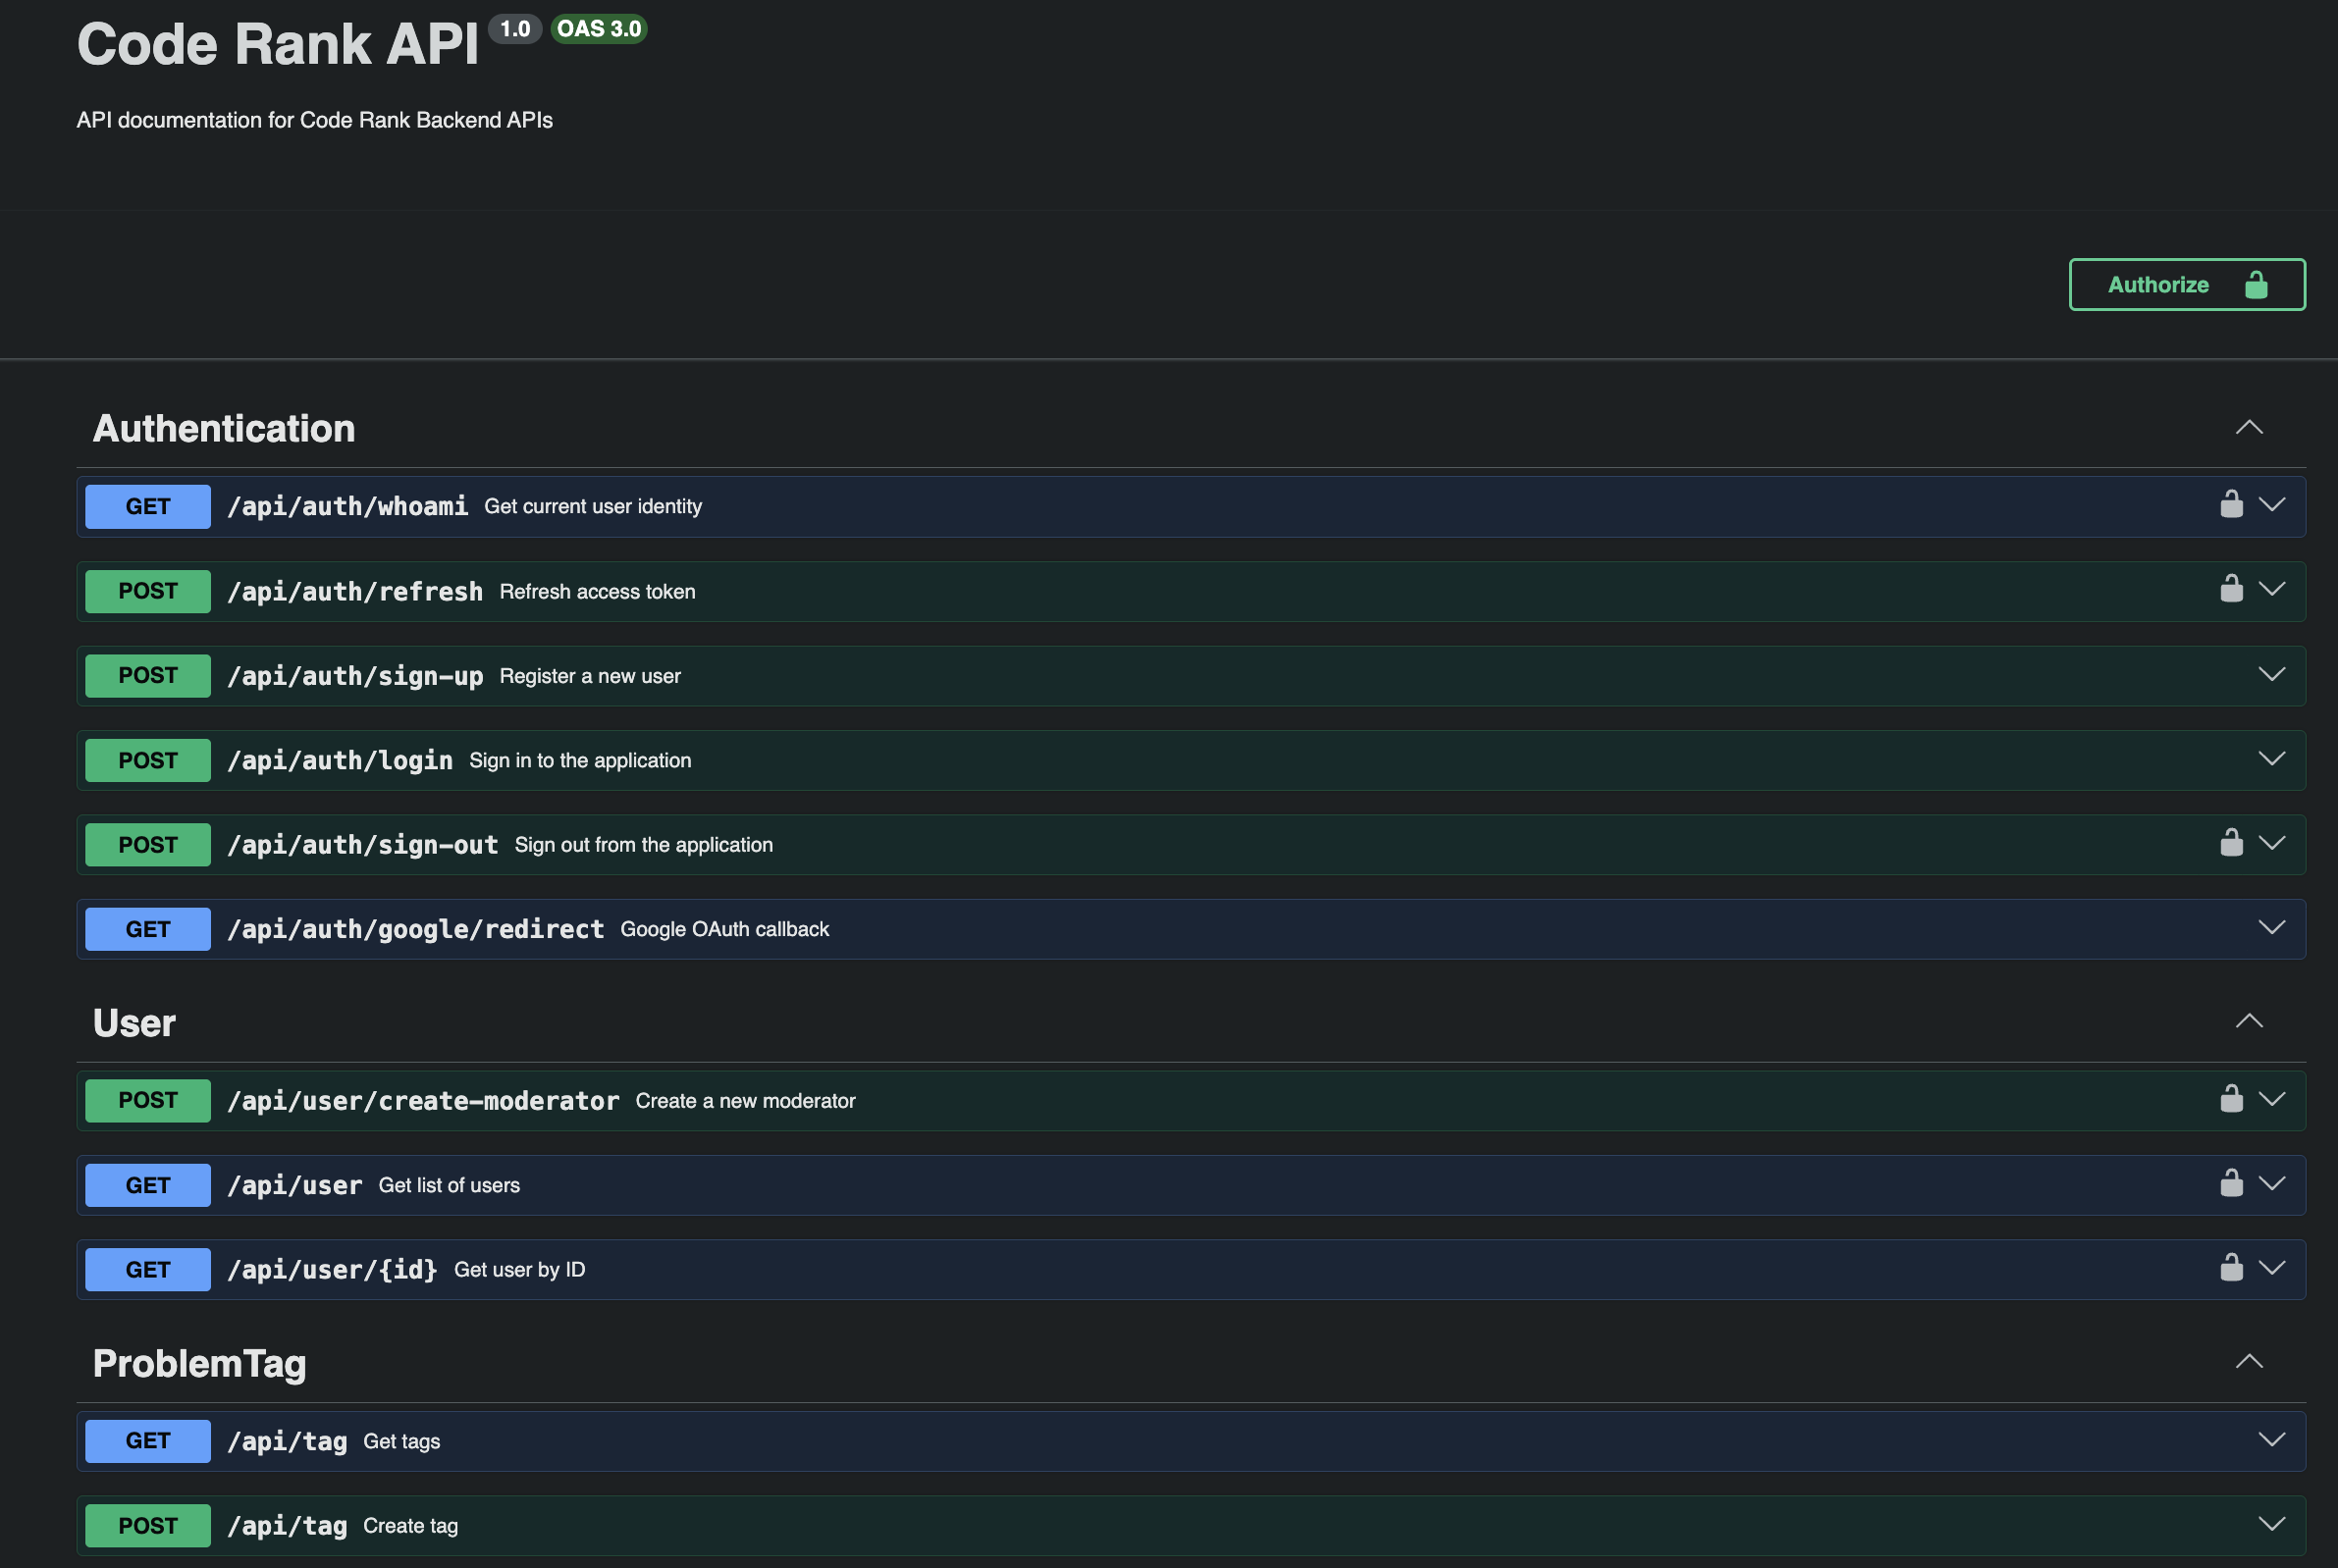
\includegraphics[width=1\textwidth]{Contents/Chapter 4/API Design/SwaggerApi.png}
    \vspace{0.6cm}
    \caption{API Swagger}
\end{figure}

\break
\section{Backend Structure}

The backend is implemented in TypeScript using a modular, Domain-Driven Design (DDD) approach built on a NestJS-style module pattern. The codebase is organized to reflect clear bounded contexts, a shared kernel for cross-cutting concerns, and an internals layer for platform services and infrastructure. This separation improves maintainability, testability, and team ownership.

\subsection{Architecture Overview}

At the highest level, the project is split into three logical layers:

\begin{enumerate}
	\item \textbf{Domain Layer}
	\item \textbf{Shared / Kernel Layer}
	\item \textbf{Internals / Infrastructure Layer}
\end{enumerate}

\subsection{Domain Layer}

This layer contains the core business logic and domain models, organized by bounded contexts under \texttt{domains}.

Each domain (for example: \texttt{auth}, \texttt{problem}, \texttt{submission}, \texttt{thread}, \texttt{user}) typically includes:

\begin{itemize}
	\item Controllers
	\item Services (use-case / application services)
	\item DTOs (Data Transfer Objects)
	\item Mappers
	\item Interfaces
	\item Domain-specific utilities
\end{itemize}

\subsection{Shared / Kernel Layer}

The shared layer contains reusable, domain-agnostic building blocks under \texttt{shared} and acts as a shared kernel to ensure reuse while keeping domain logic decoupled from framework specifics.

It includes:

\begin{itemize}
	\item Aggregate root patterns (e.g. \texttt{shared/aggregate})
	\item Base entities (e.g. \texttt{shared/entity})
	\item Common exceptions and constants
	\item Generic mappers
\end{itemize}

\subsection{Internals / Infrastructure Layer}

This layer contains platform-level concerns and infrastructure adapters under \texttt{internals}.

Common responsibilities:

\begin{itemize}
	\item Configuration (for example, \texttt{configuration.ts})
	\item Database setup and entity wiring (\texttt{database})
	\item Core framework services (\texttt{core})
	\item Infrastructure integrations (message brokers, external systems)
\end{itemize}

\subsection{Bounded Contexts and Module Responsibilities}

Each domain module represents a bounded context with clear ownership of its business logic.

\subsubsection{Auth Module}
\begin{itemize}
    \item Register and authenticate users (sign-up / sign-in).
    \item Issue, refresh, and revoke tokens / sessions.
    \item Validate and authorize requests based on roles/permissions.
    \item Enforce authentication-related business rules (e.g., account linking, password policies).
\end{itemize}


\subsubsection{Chatbot Module}
\begin{itemize}
    \item Intended to handle CRUD for AI conversation lifecycle (messages, sessions, histories).
    \item Acts as an adapter between HTTP controllers and an AI agent service (conversation orchestration).
    \item Stores or references conversation state and metadata for retrieval and continuation.
    \item Handle async processing and retries for AI responses.
    \item Integrates with infrastructure for calling external AI APIs and with message brokers for async tasks.
\end{itemize}

\subsubsection{Problem Module}
\begin{itemize}
    \item Create, update, publish, and archive problems.
    \item Manage problem metadata (tags, testcases, difficulty, reviews).
    \item Provide read models for public consumption and management views for editors.
    \item Validate problem inputs and maintain consistency of testcases and constraints.
\end{itemize}

\subsubsection{Submission Module}
\begin{itemize}
    \item Accept and record solution submissions from users.
    \item Queue and coordinate evaluation / judging workflows.
    \item Store and expose submission results, logs, and execution metadata.
    \item Handle retries, timeouts, and result aggregation for judging.
\end{itemize}

\subsubsection{Thread Module}
\begin{itemize}
    \item Create and manage discussions and comment threads.
    \item Support reactions/likes and moderation actions (edit/delete/report).
    \item Query and paginate discussions, comments, and thread metadata.
    \item Enforce posting rules and notification triggers for thread activity.
\end{itemize}

\subsubsection{User Module}
\begin{itemize}
    \item Manage user profiles, settings, and preferences.
    \item Handle user registration, authentication, and authorization.
    \item Provide user listing, search, and administrative controls.
    \item Enforce privacy, role-based access, and moderation policies.
\end{itemize}

\break
\section{Chatbot Implementation}

This section describes the detailed implementation of the chatbot subsystem in the CodeRank system. The implementation focuses on enabling real-time, streaming-based conversational interaction between the user and the AI assistant.

The chatbot is implemented using a multi-layer architecture consisting of the frontend client, backend API server, n8n workflow engine, and Gemini large language model. A key feature of the system is the use of Server-Sent Events (SSE) to support streaming responses, providing a real-time chat experience similar to modern AI assistants.

\subsection{End-to-End Chatbot Request Flow}

When a user interacts with the chatbot, the system processes the request through the following sequence:

\begin{enumerate}
    \item The user submits a message from the frontend chatbot interface.
    
    \item The frontend immediately sends the message to the backend API server using an HTTP request.
    
    \item The backend receives the request and initiates a processing pipeline by calling an internal chatbot service.
    
    \item The backend triggers an n8n workflow via a webhook, passing the user input and conversation metadata.
    
    \item n8n processes the request and communicates with the Gemini model to generate a response.
    
    \item The response is streamed back from n8n to the backend.
    
    \item The backend forwards the streamed response to the frontend using Server-Sent Events (SSE).
    
    \item The frontend renders the response incrementally in real time as tokens are received.
\end{enumerate}

This architecture ensures low-latency interaction and improves user experience by allowing the response to appear progressively instead of waiting for the full output.

\subsection{Backend Processing and Streaming Architecture}

The backend plays a critical role in managing request orchestration and enabling real-time response streaming.

After receiving the request from the frontend, the backend does not wait for the full response from the AI pipeline. Instead, it establishes a Server-Sent Events (SSE) connection with the client and acts as a streaming proxy between n8n and the frontend.

The backend performs the following tasks:

\begin{itemize}
    \item Validates incoming chatbot requests
    \item Forwards the request to the n8n webhook endpoint
    \item Receives streamed response chunks from n8n
    \item Forwards each chunk to the frontend via SSE channel
\end{itemize}

This streaming mechanism allows the system to handle long AI-generated responses efficiently while maintaining responsiveness.

\subsection{n8n Workflow Execution and Streaming Response}

Within the n8n workflow, the chatbot request is processed through multiple stages including context retrieval, prompt construction, and LLM inference.

Unlike traditional synchronous APIs, the integration is designed to support incremental response generation. As the Gemini model produces output, n8n streams partial results back to the backend instead of waiting for the full completion.

This streaming behavior is essential for enabling real-time chat experiences and reducing perceived latency.

The workflow acts as an intermediate layer that:
\begin{itemize}
    \item Receives user input from the backend via webhook
    \item Processes conversational context and memory
    \item Sends structured prompts to the Gemini model
    \item Streams generated tokens or response chunks back to the backend
\end{itemize}

\subsection{Frontend Streaming with Server-Sent Events (SSE)}

On the frontend side, the chatbot interface establishes a persistent SSE connection with the backend.

When a user sends a message, the frontend immediately displays a loading state and begins listening for streamed response events.

As the backend receives chunks of data from n8n, it forwards them to the frontend incrementally. The frontend then appends each received chunk to the chat interface in real time.

This results in a typewriter-like effect where the response appears progressively, significantly improving user experience compared to traditional request-response models.

The SSE-based approach provides the following benefits:
\begin{itemize}
    \item Low latency response rendering
    \item Improved perceived system performance
    \item Smooth real-time interaction experience
    \item Reduced waiting time for long AI outputs
\end{itemize}

\section{Mockup Design}

Mockup Design is a low-fidelity visual representation of a user interface that outlines the basic structure and layout of a digital product without focusing on visual design elements such as colors, typography, or imagery. Mockup Designs serve as a blueprint for developers and designers, defining the placement of content, navigation elements, and interactive components. This section will cover the Mockup Designs for two main user flows: \textit{Primary User flow} and \textit{Moderator/Admin flow} .

\subsection{Primary User flow}
\subsubsection*{Login}

Before accessing the application, users are required to login using their credentials. The Login Page will include 2 options based on role: Moderator/Admin login and User login.
\begin{figure}[H]
    \centering
    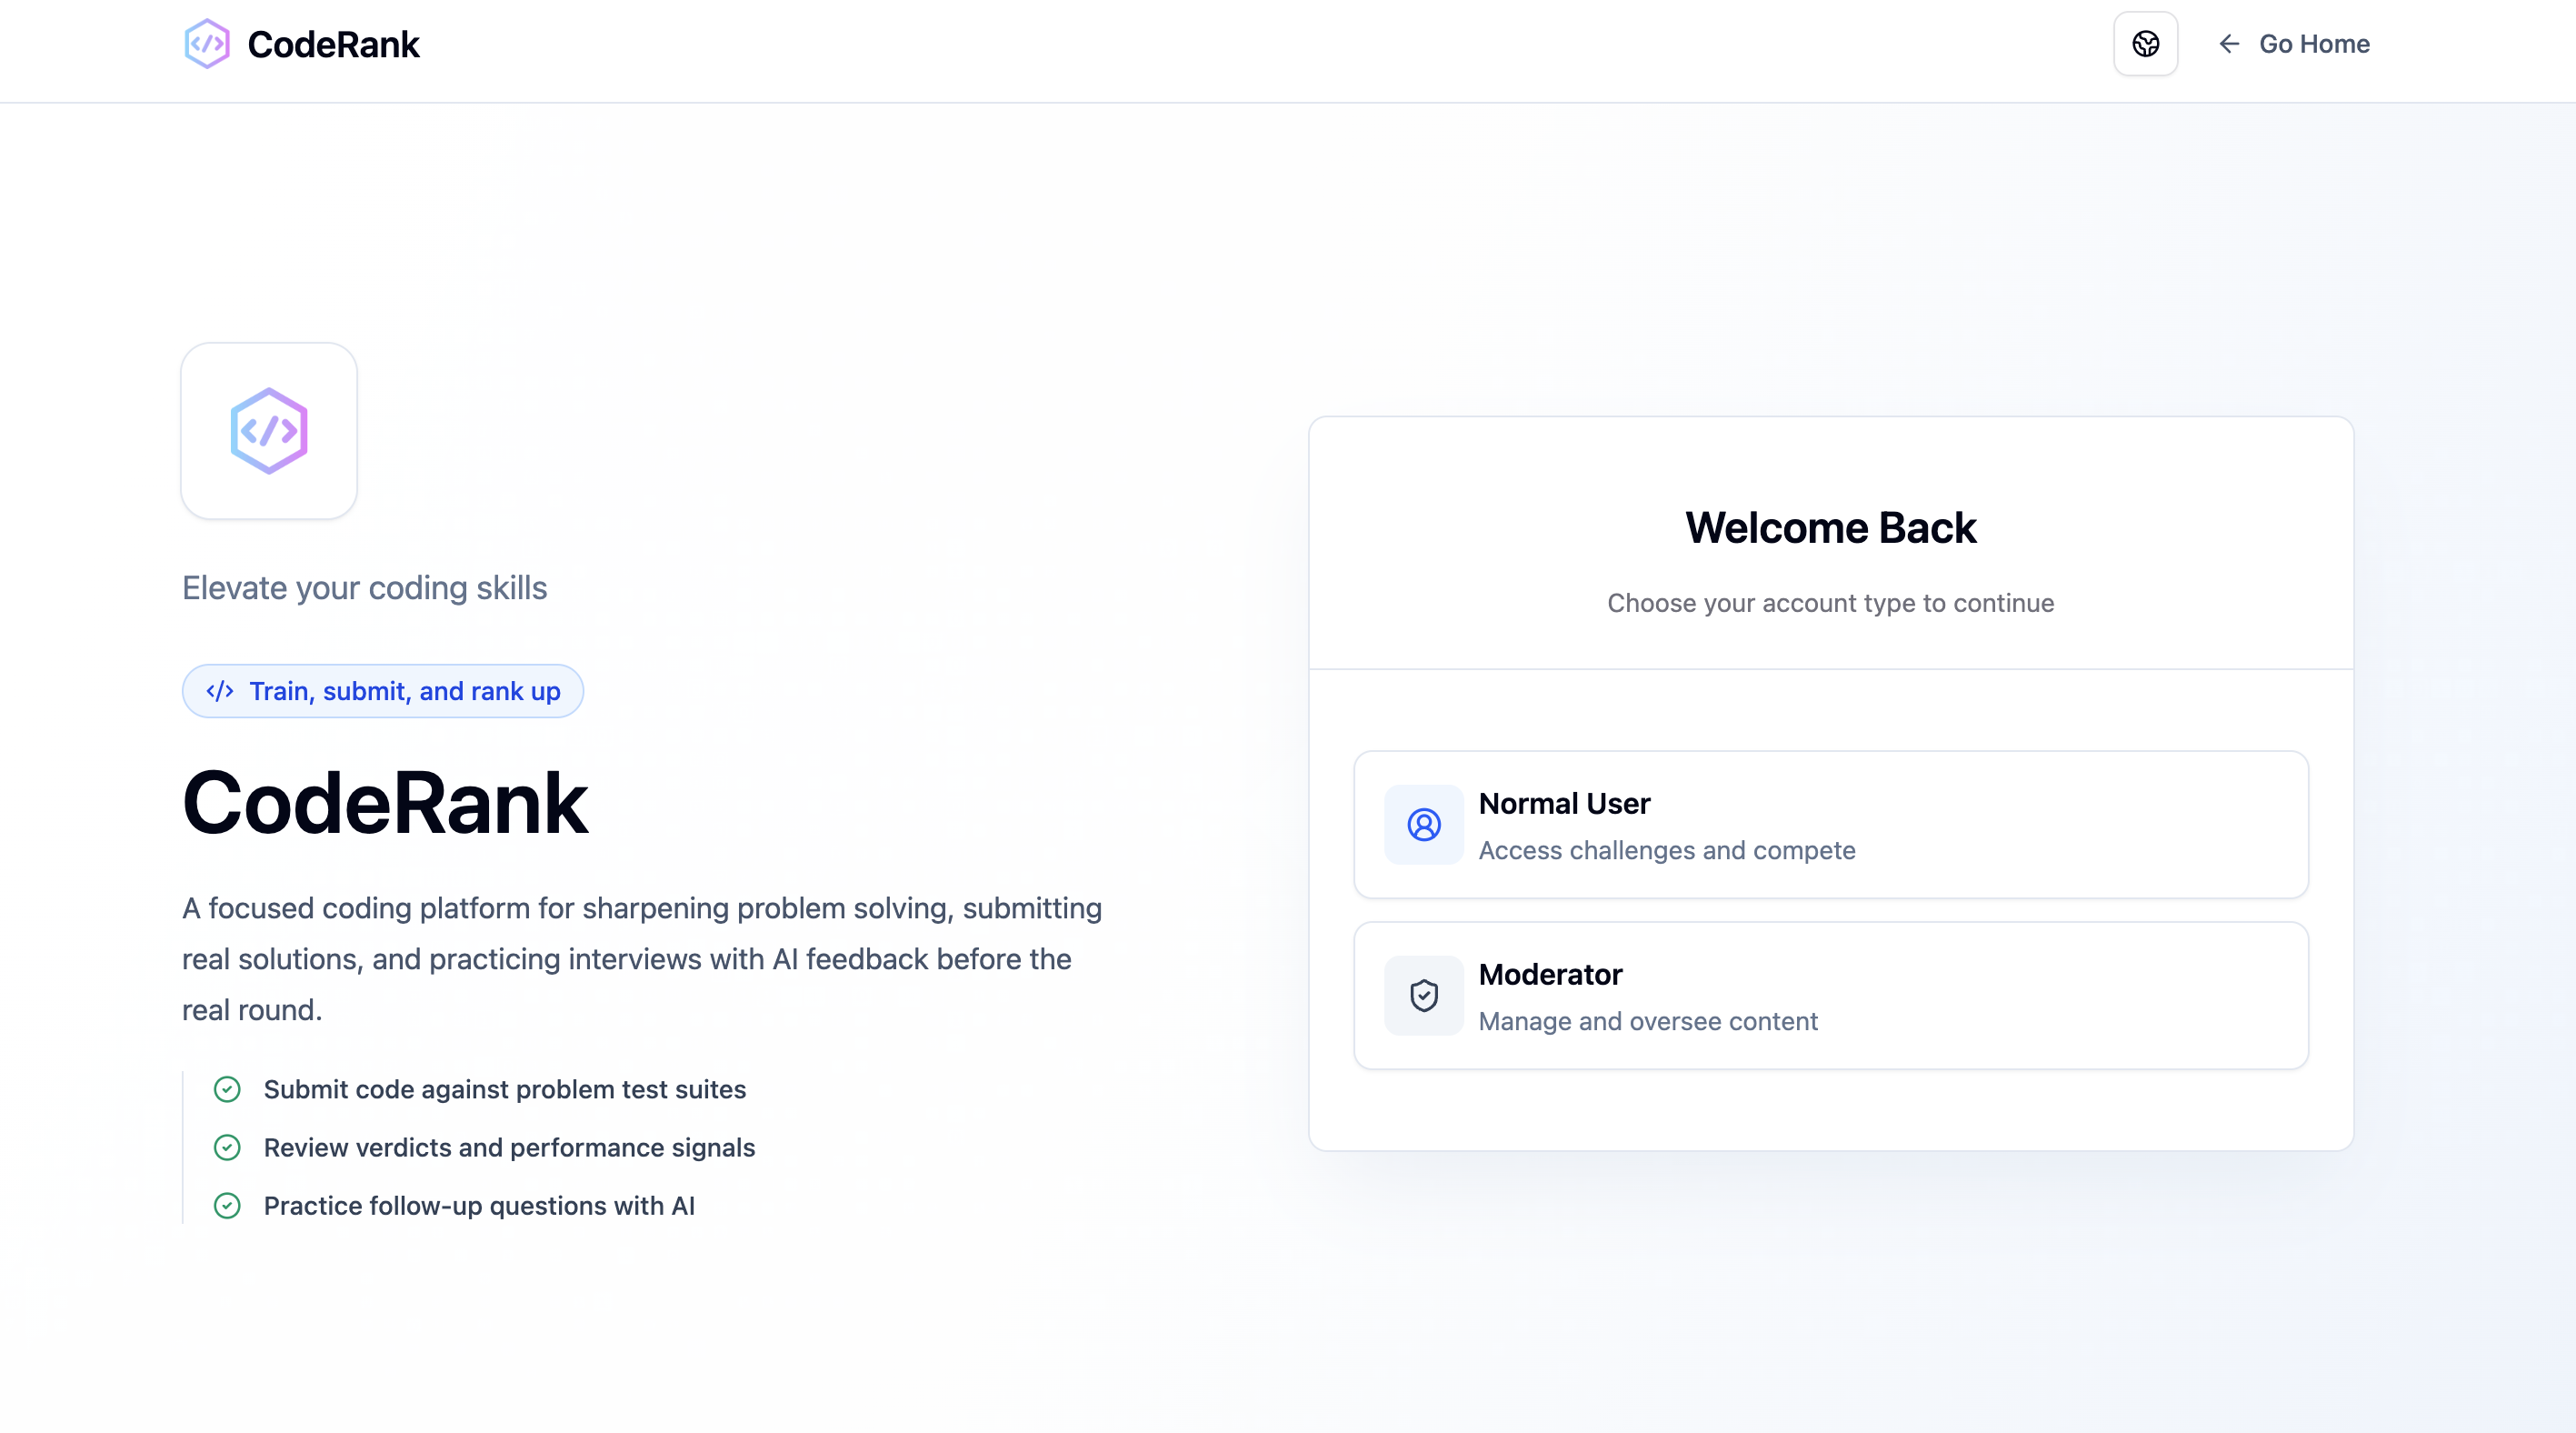
\includegraphics[width=1\textwidth]{Contents/Chapter 4/Mockup Design/Primary User/login_selection.png}
    \vspace{0.6cm}
    \caption{Login Page \- Role Selection}
\end{figure}

For Primary User, after selecting User login, the user will be directed to the User Login Page. This will include fields for entering username and password, along with a login button. There is also an option for login vie Google OAuth. After login successful, there will be a toast notification indicating success and redirecting to the Problem List page. Any validation errors will be displayed in the below of the corresponding input fields if the user enters incorrect credentials.
\begin{figure}[H]
    \centering
    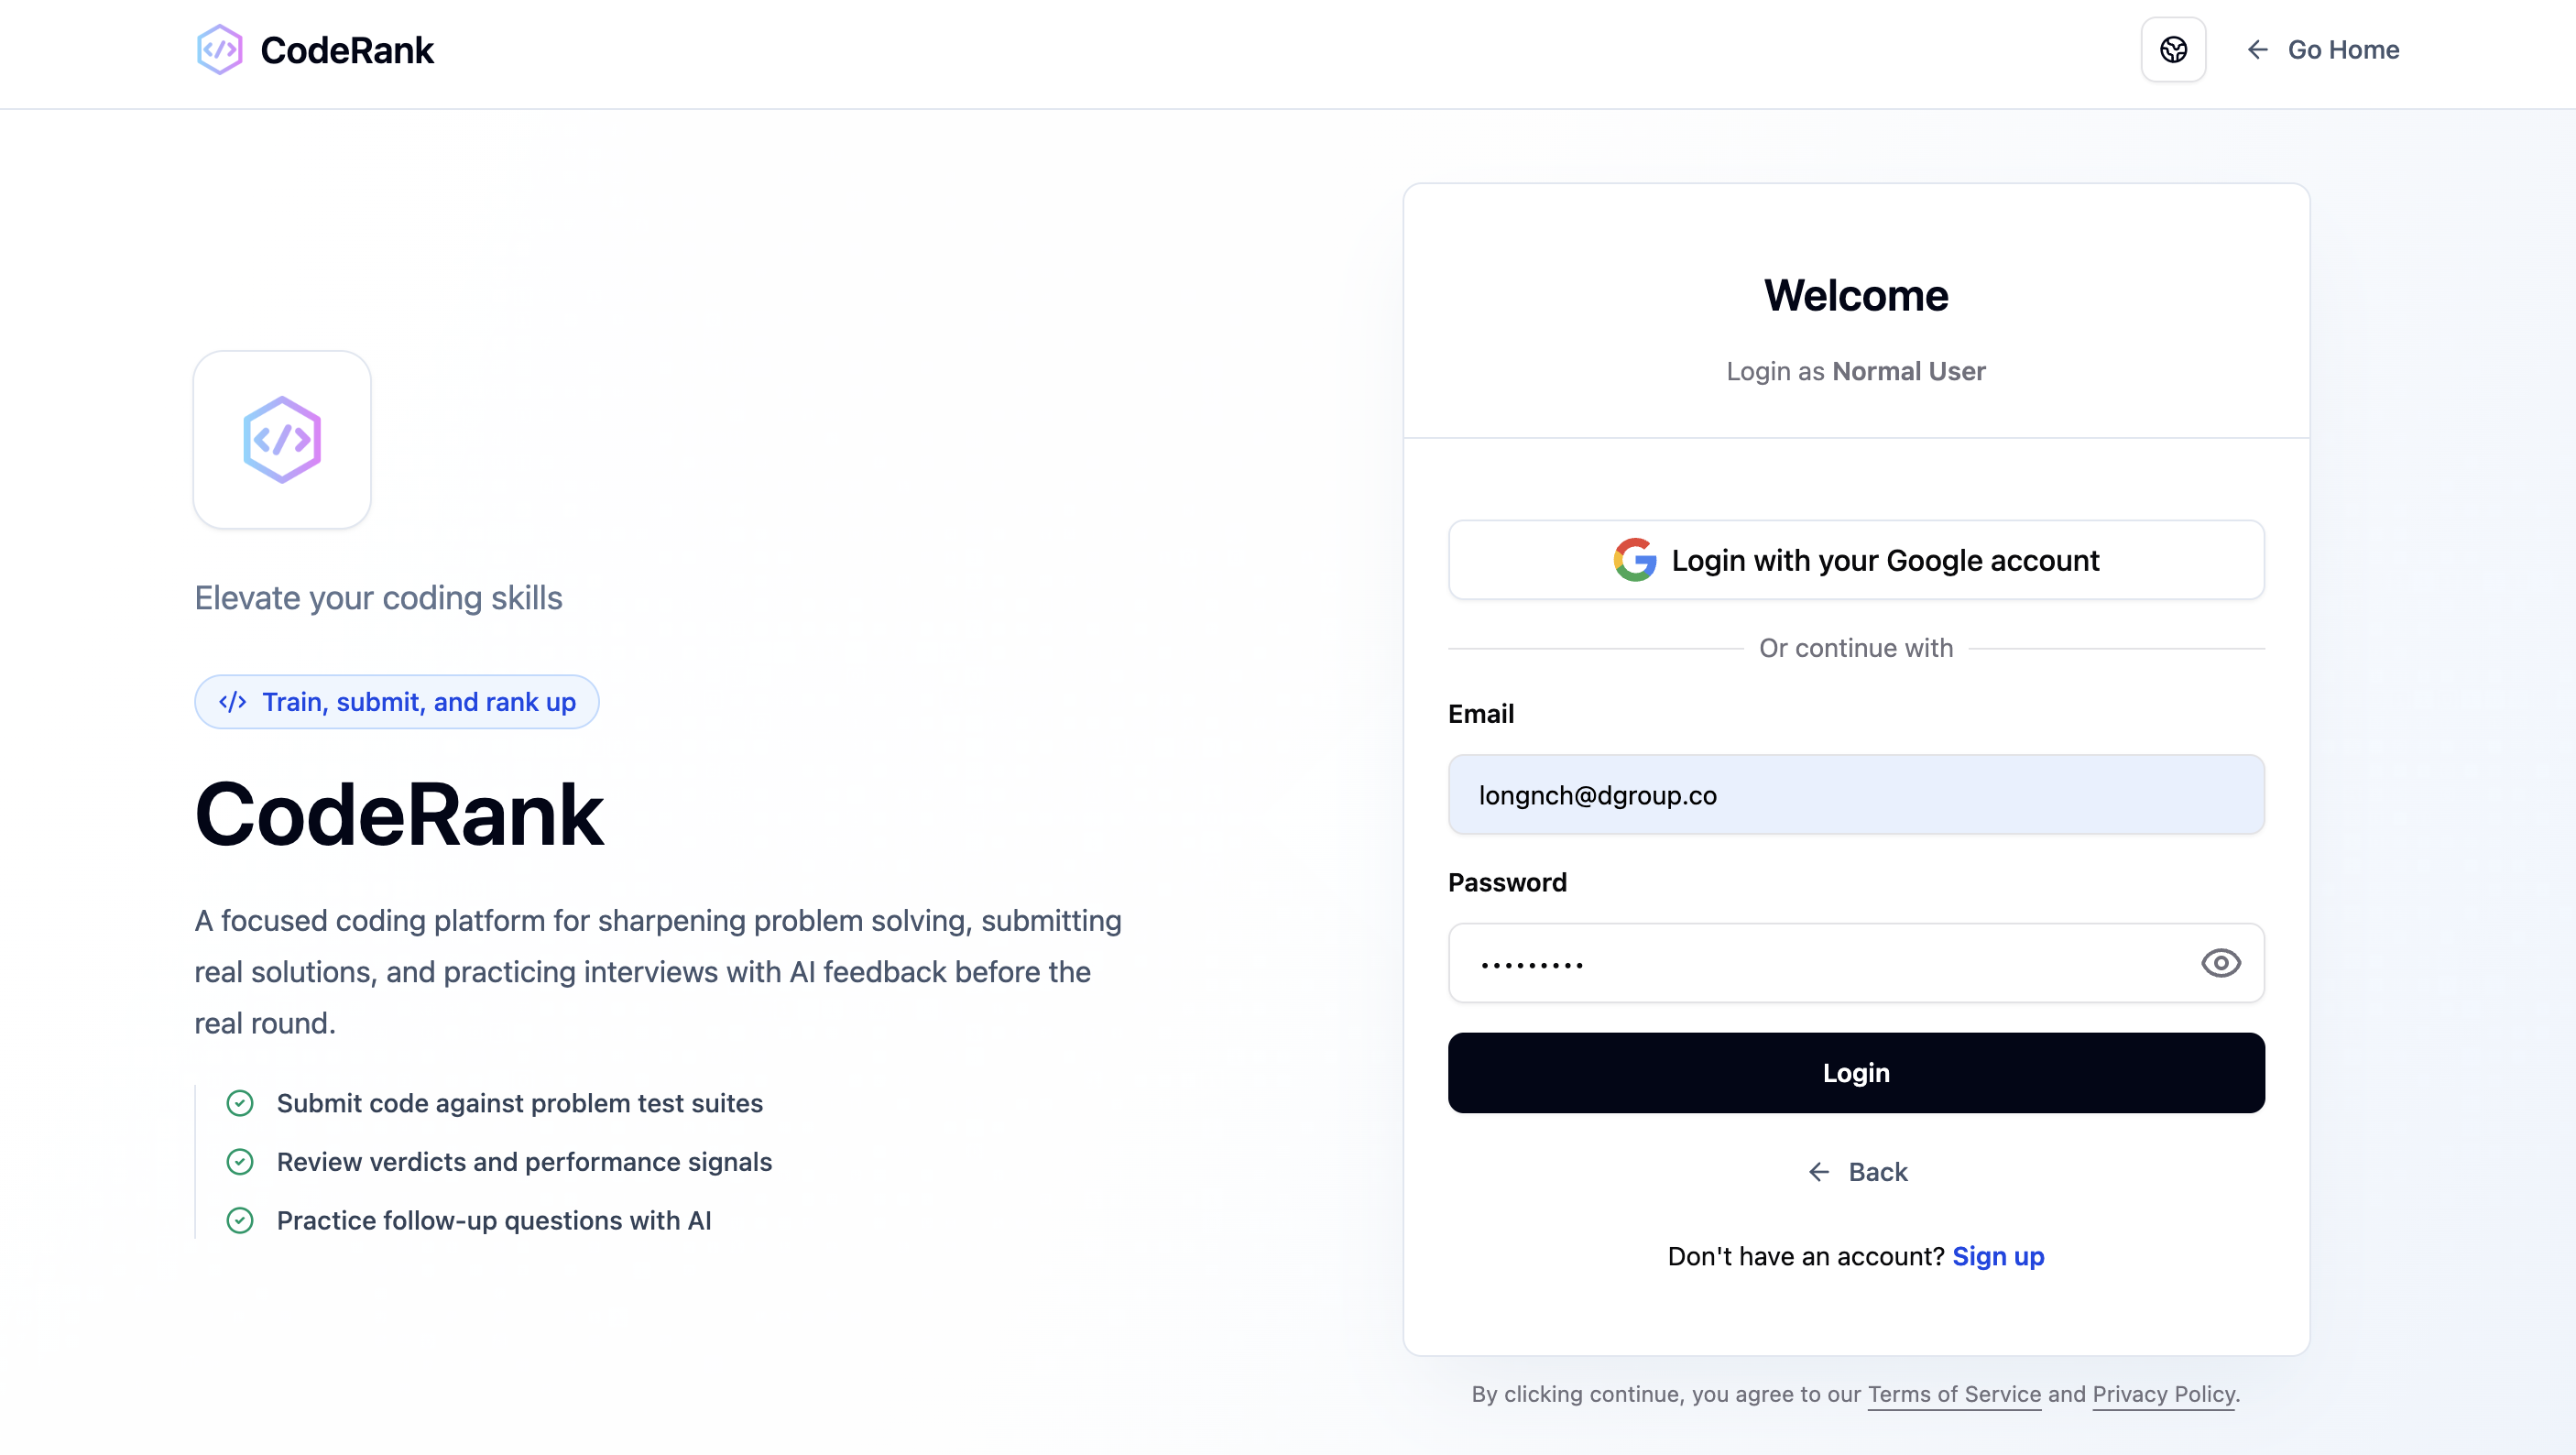
\includegraphics[width=1\textwidth]{Contents/Chapter 4/Mockup Design/Primary User/login_primary.png}
    \vspace{0.6cm}
    \caption{Login Page \- Primary User Login}
\end{figure}

\subsubsubsection*{Problem List}
After logging in, the Primary User will be directed to the Problem List page. This page displays a list of coding problems available on the platform, along with relevant details such as problem title, difficulty level, and tags. Users can filter and sort the problems based on various criteria to find specific challenges they want to solve.
\begin{figure}[H]
    \centering
    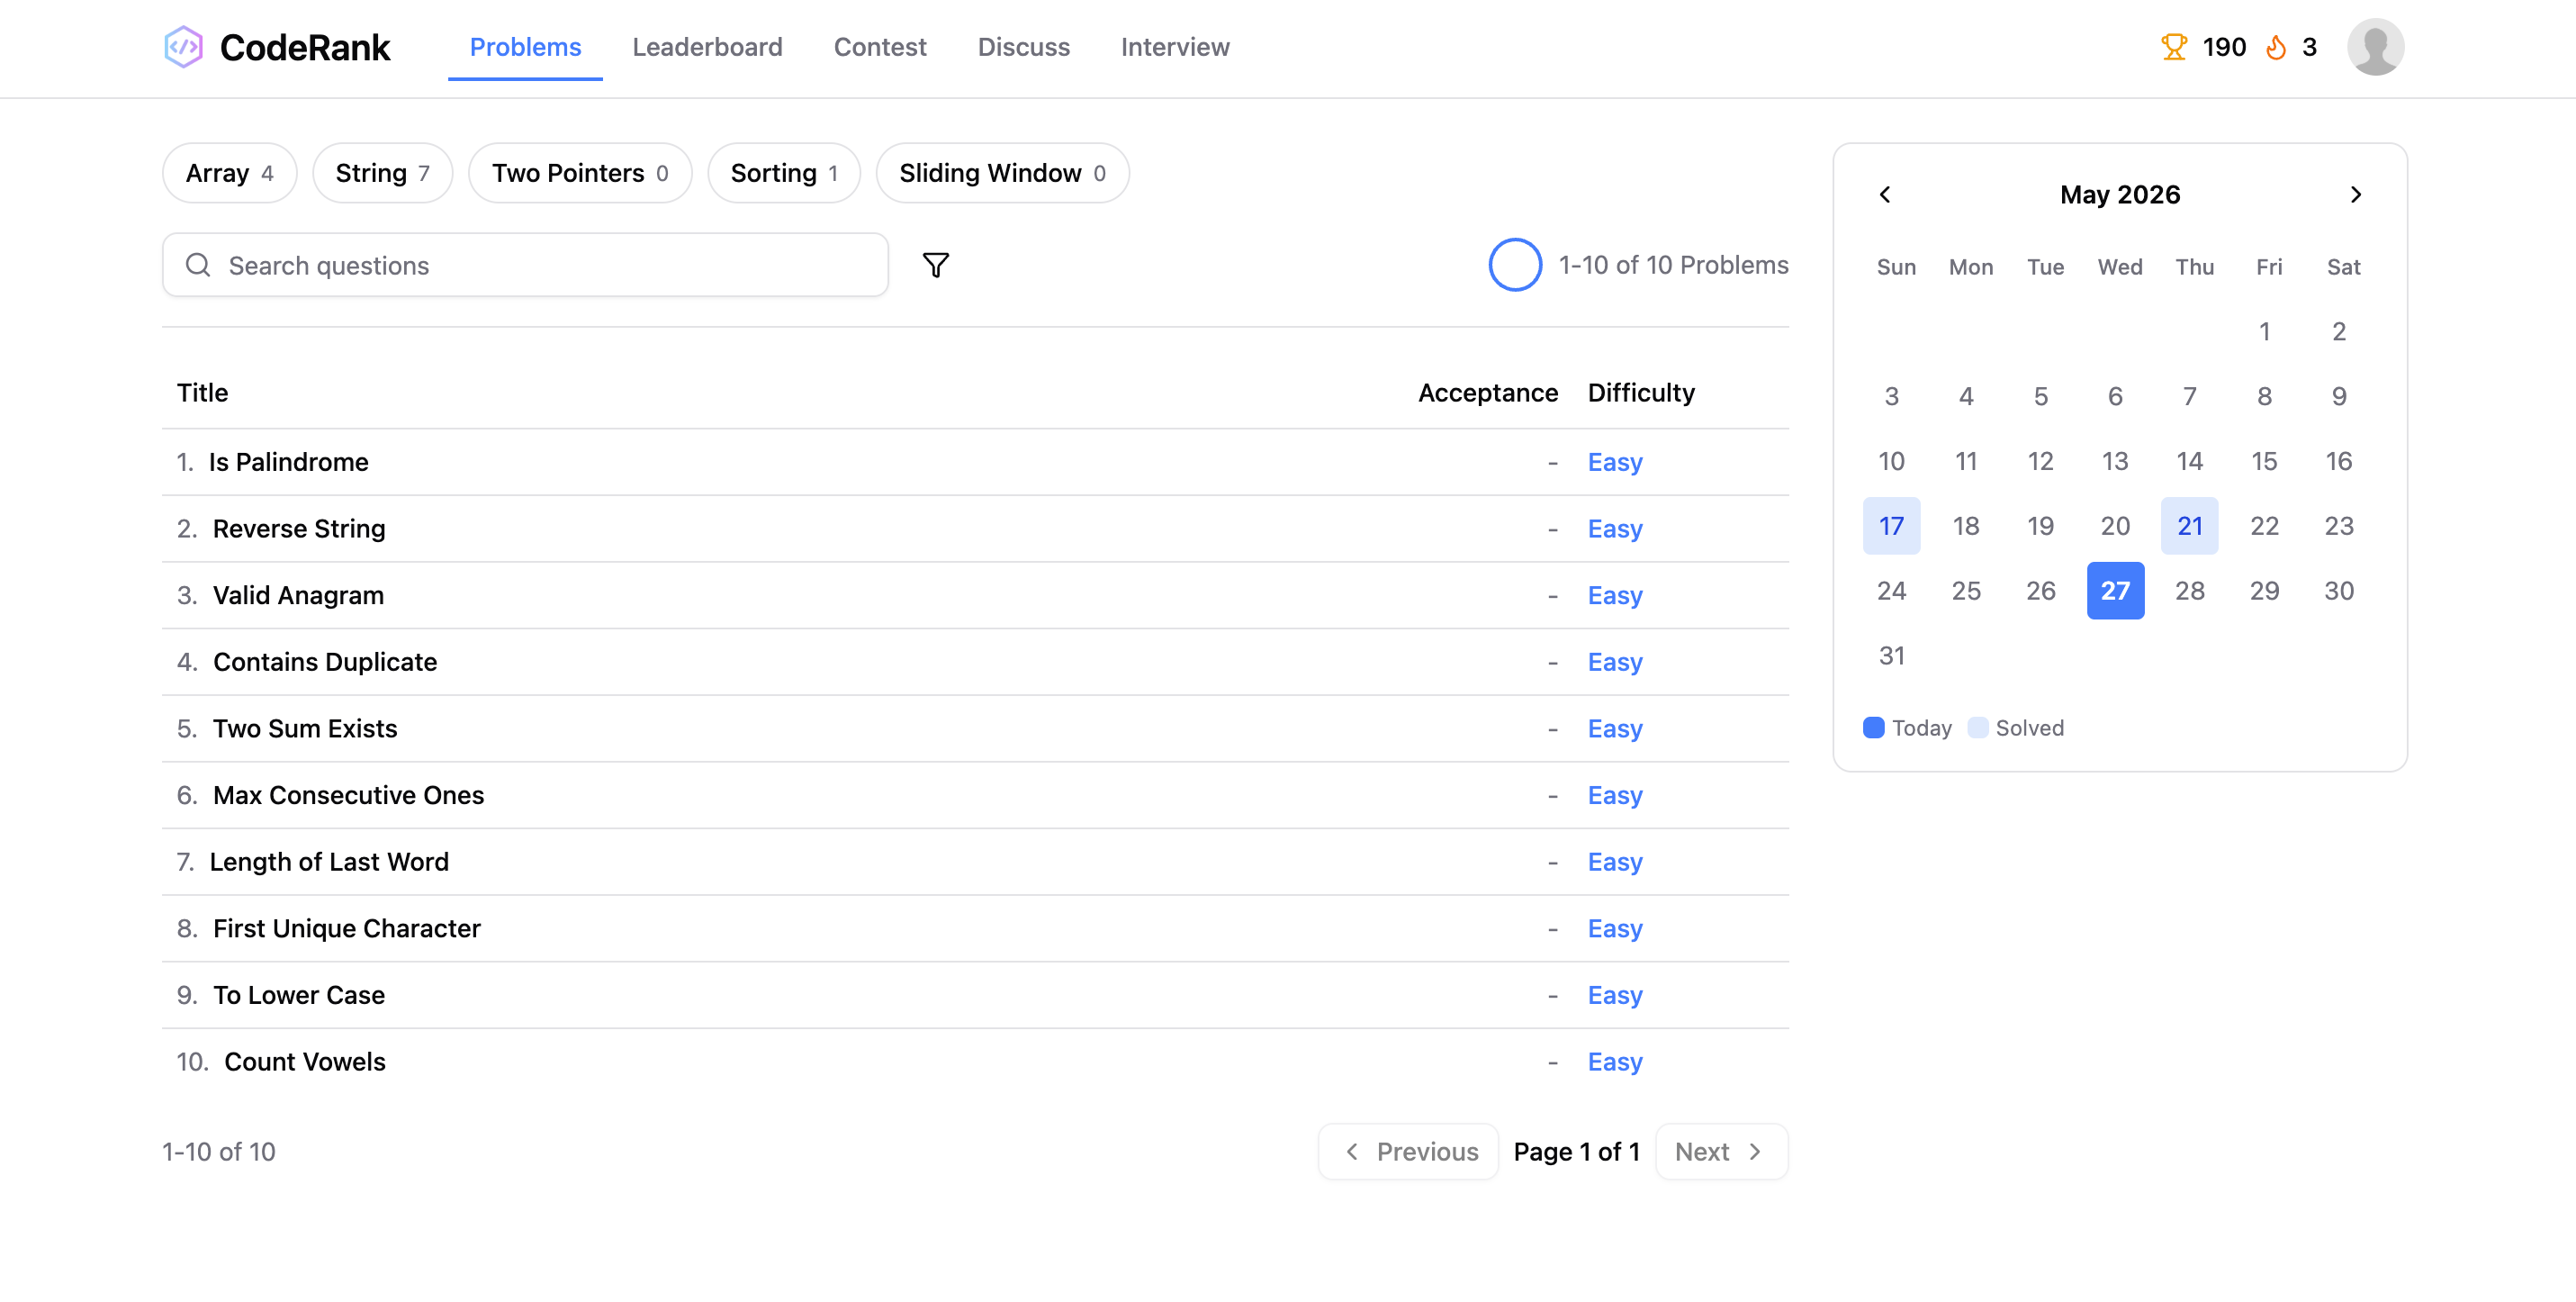
\includegraphics[width=1\textwidth]{Contents/Chapter 4/Mockup Design/Primary User/problem_list.png}
    \vspace{0.6cm}
    \caption{Problem List page}
\end{figure}

The Problem List page also includes a search bar at the top, allowing users to quickly search for problems by keywords or tags. Each problem entry in the list is clickable, leading to the Problem Detail page where users can view the full problem description and submit their solutions.
\begin{figure}[H]
    \centering
    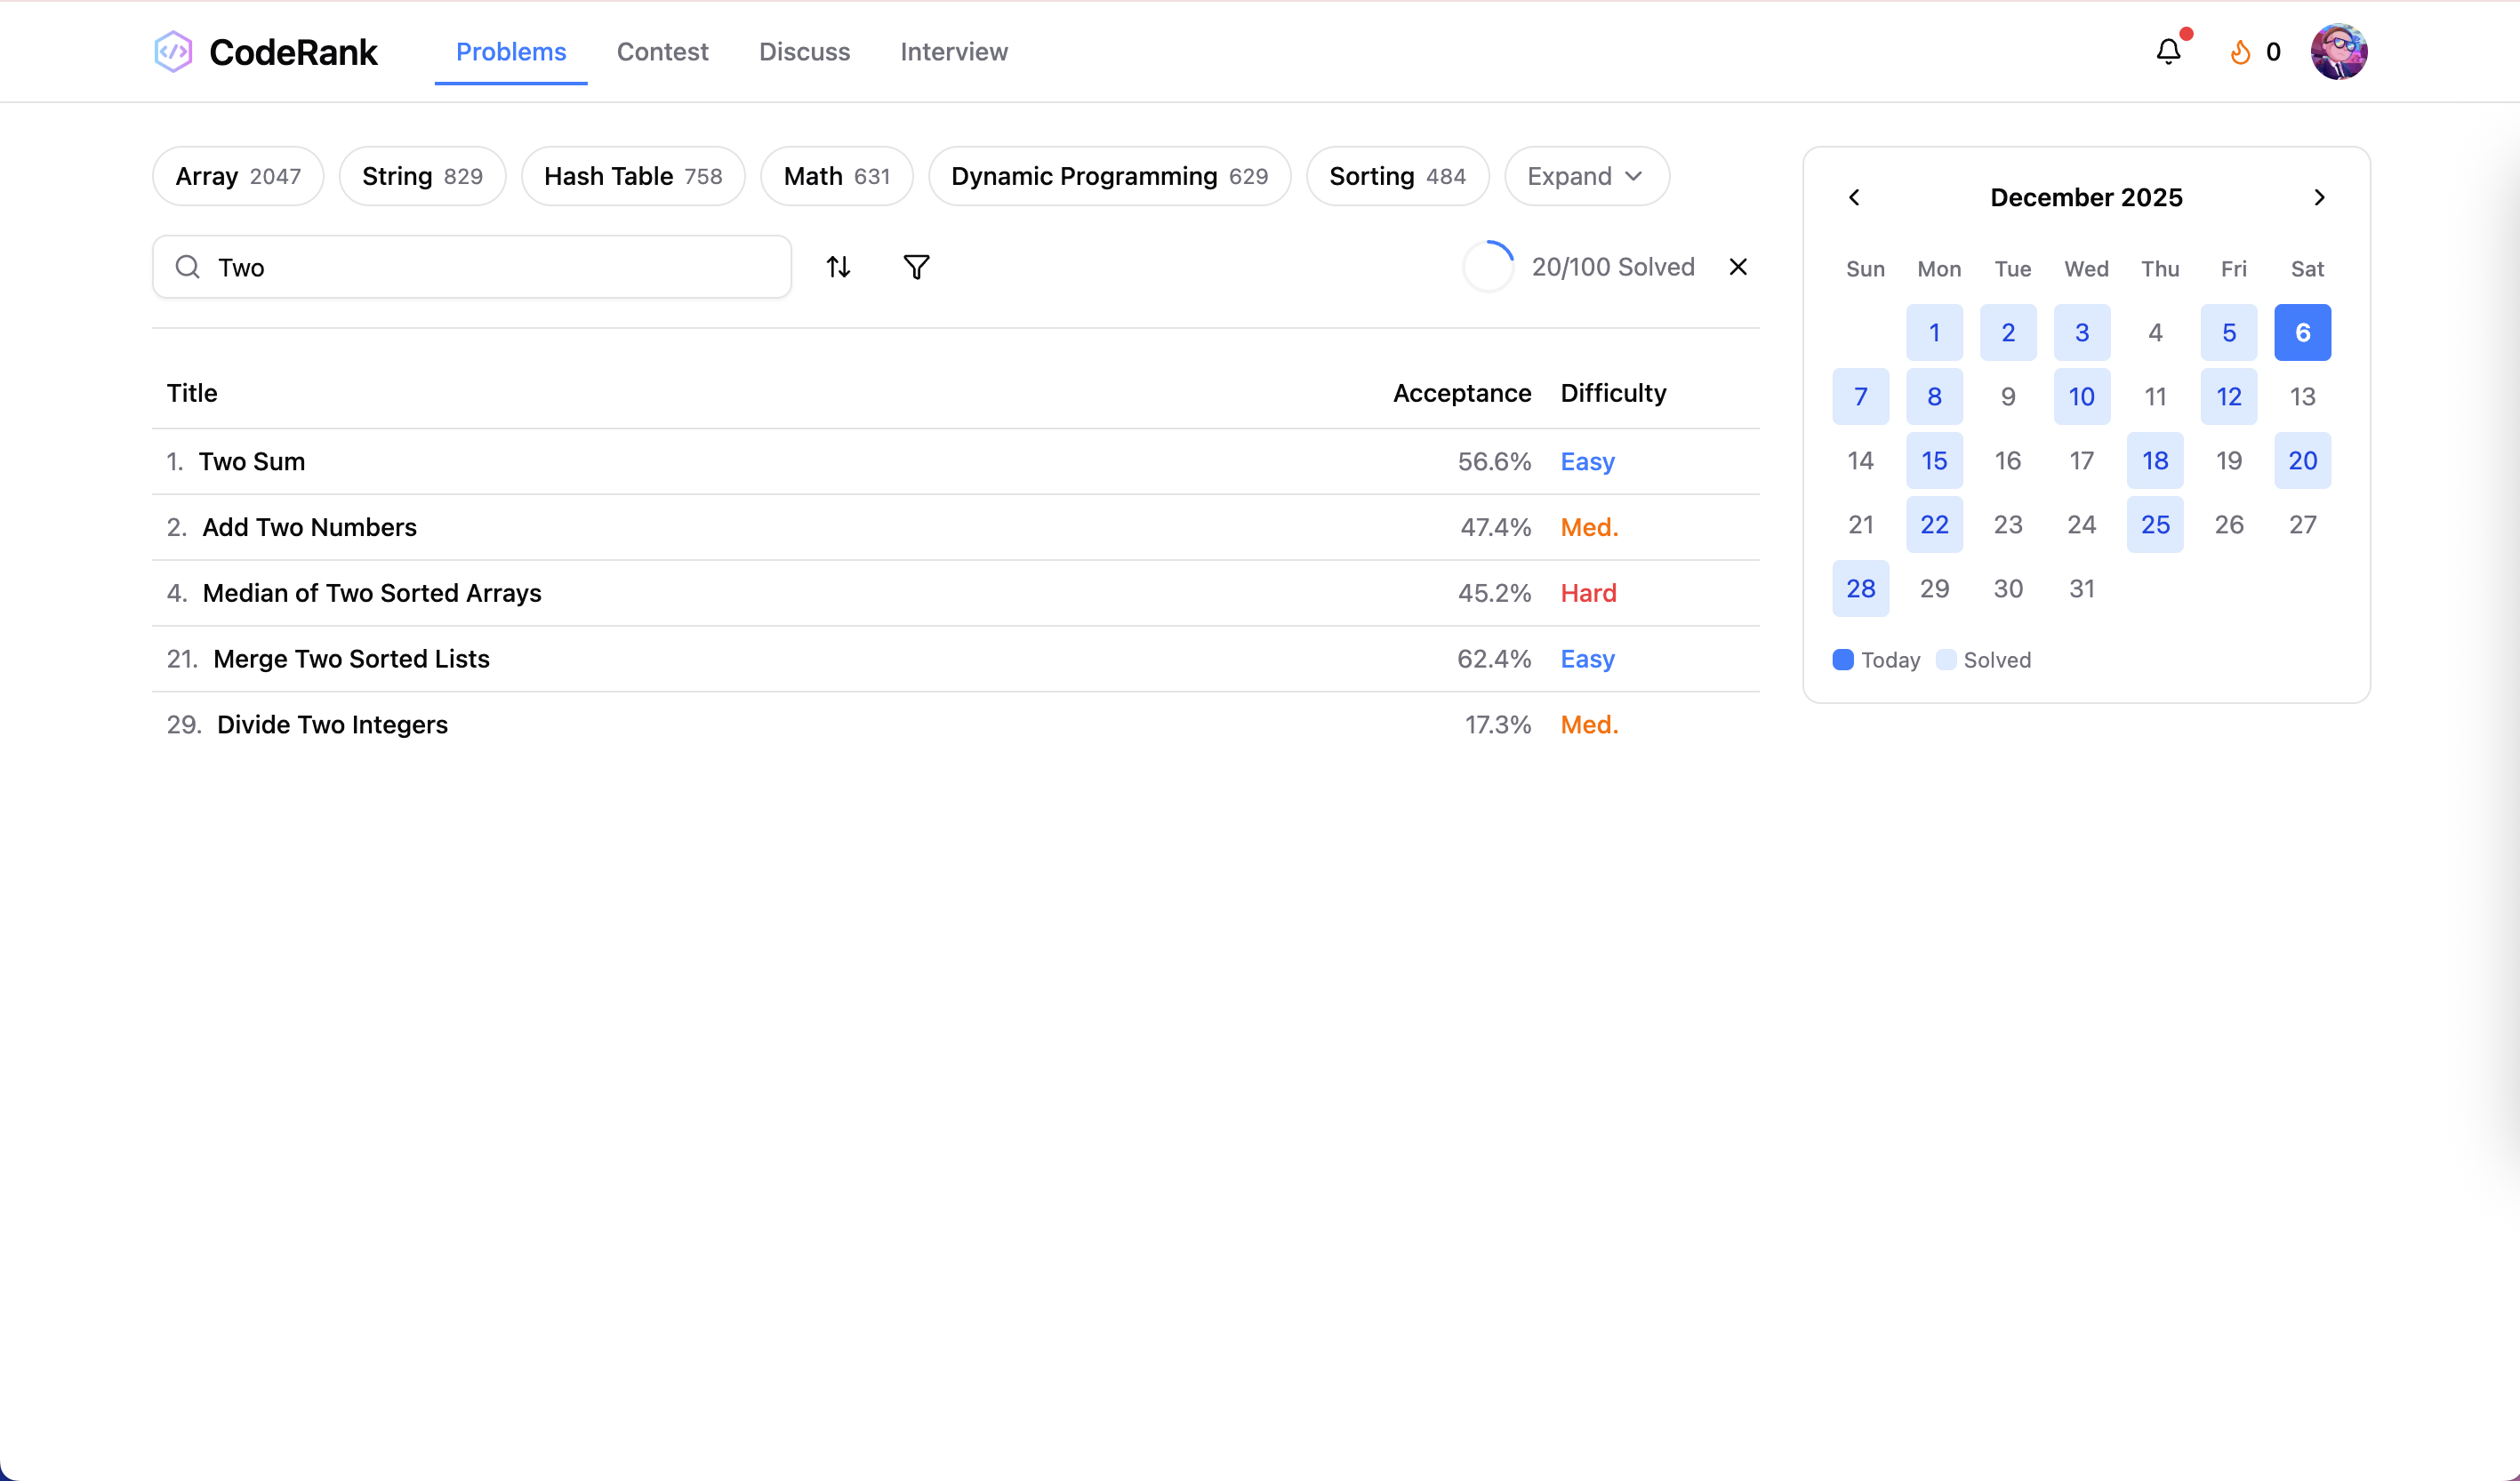
\includegraphics[width=1\textwidth]{Contents/Chapter 4/Mockup Design/Primary User/problem_list_search.png}
    \vspace{0.6cm}
    \caption{Problem List Search}
\end{figure}

In order to solve a problem, the user can click on the problem title in the Problem List. This will take them to the Problem Detail page, where they can read the problem description, view constraints, and submit their code solution.
\begin{figure}[H]
    \centering
    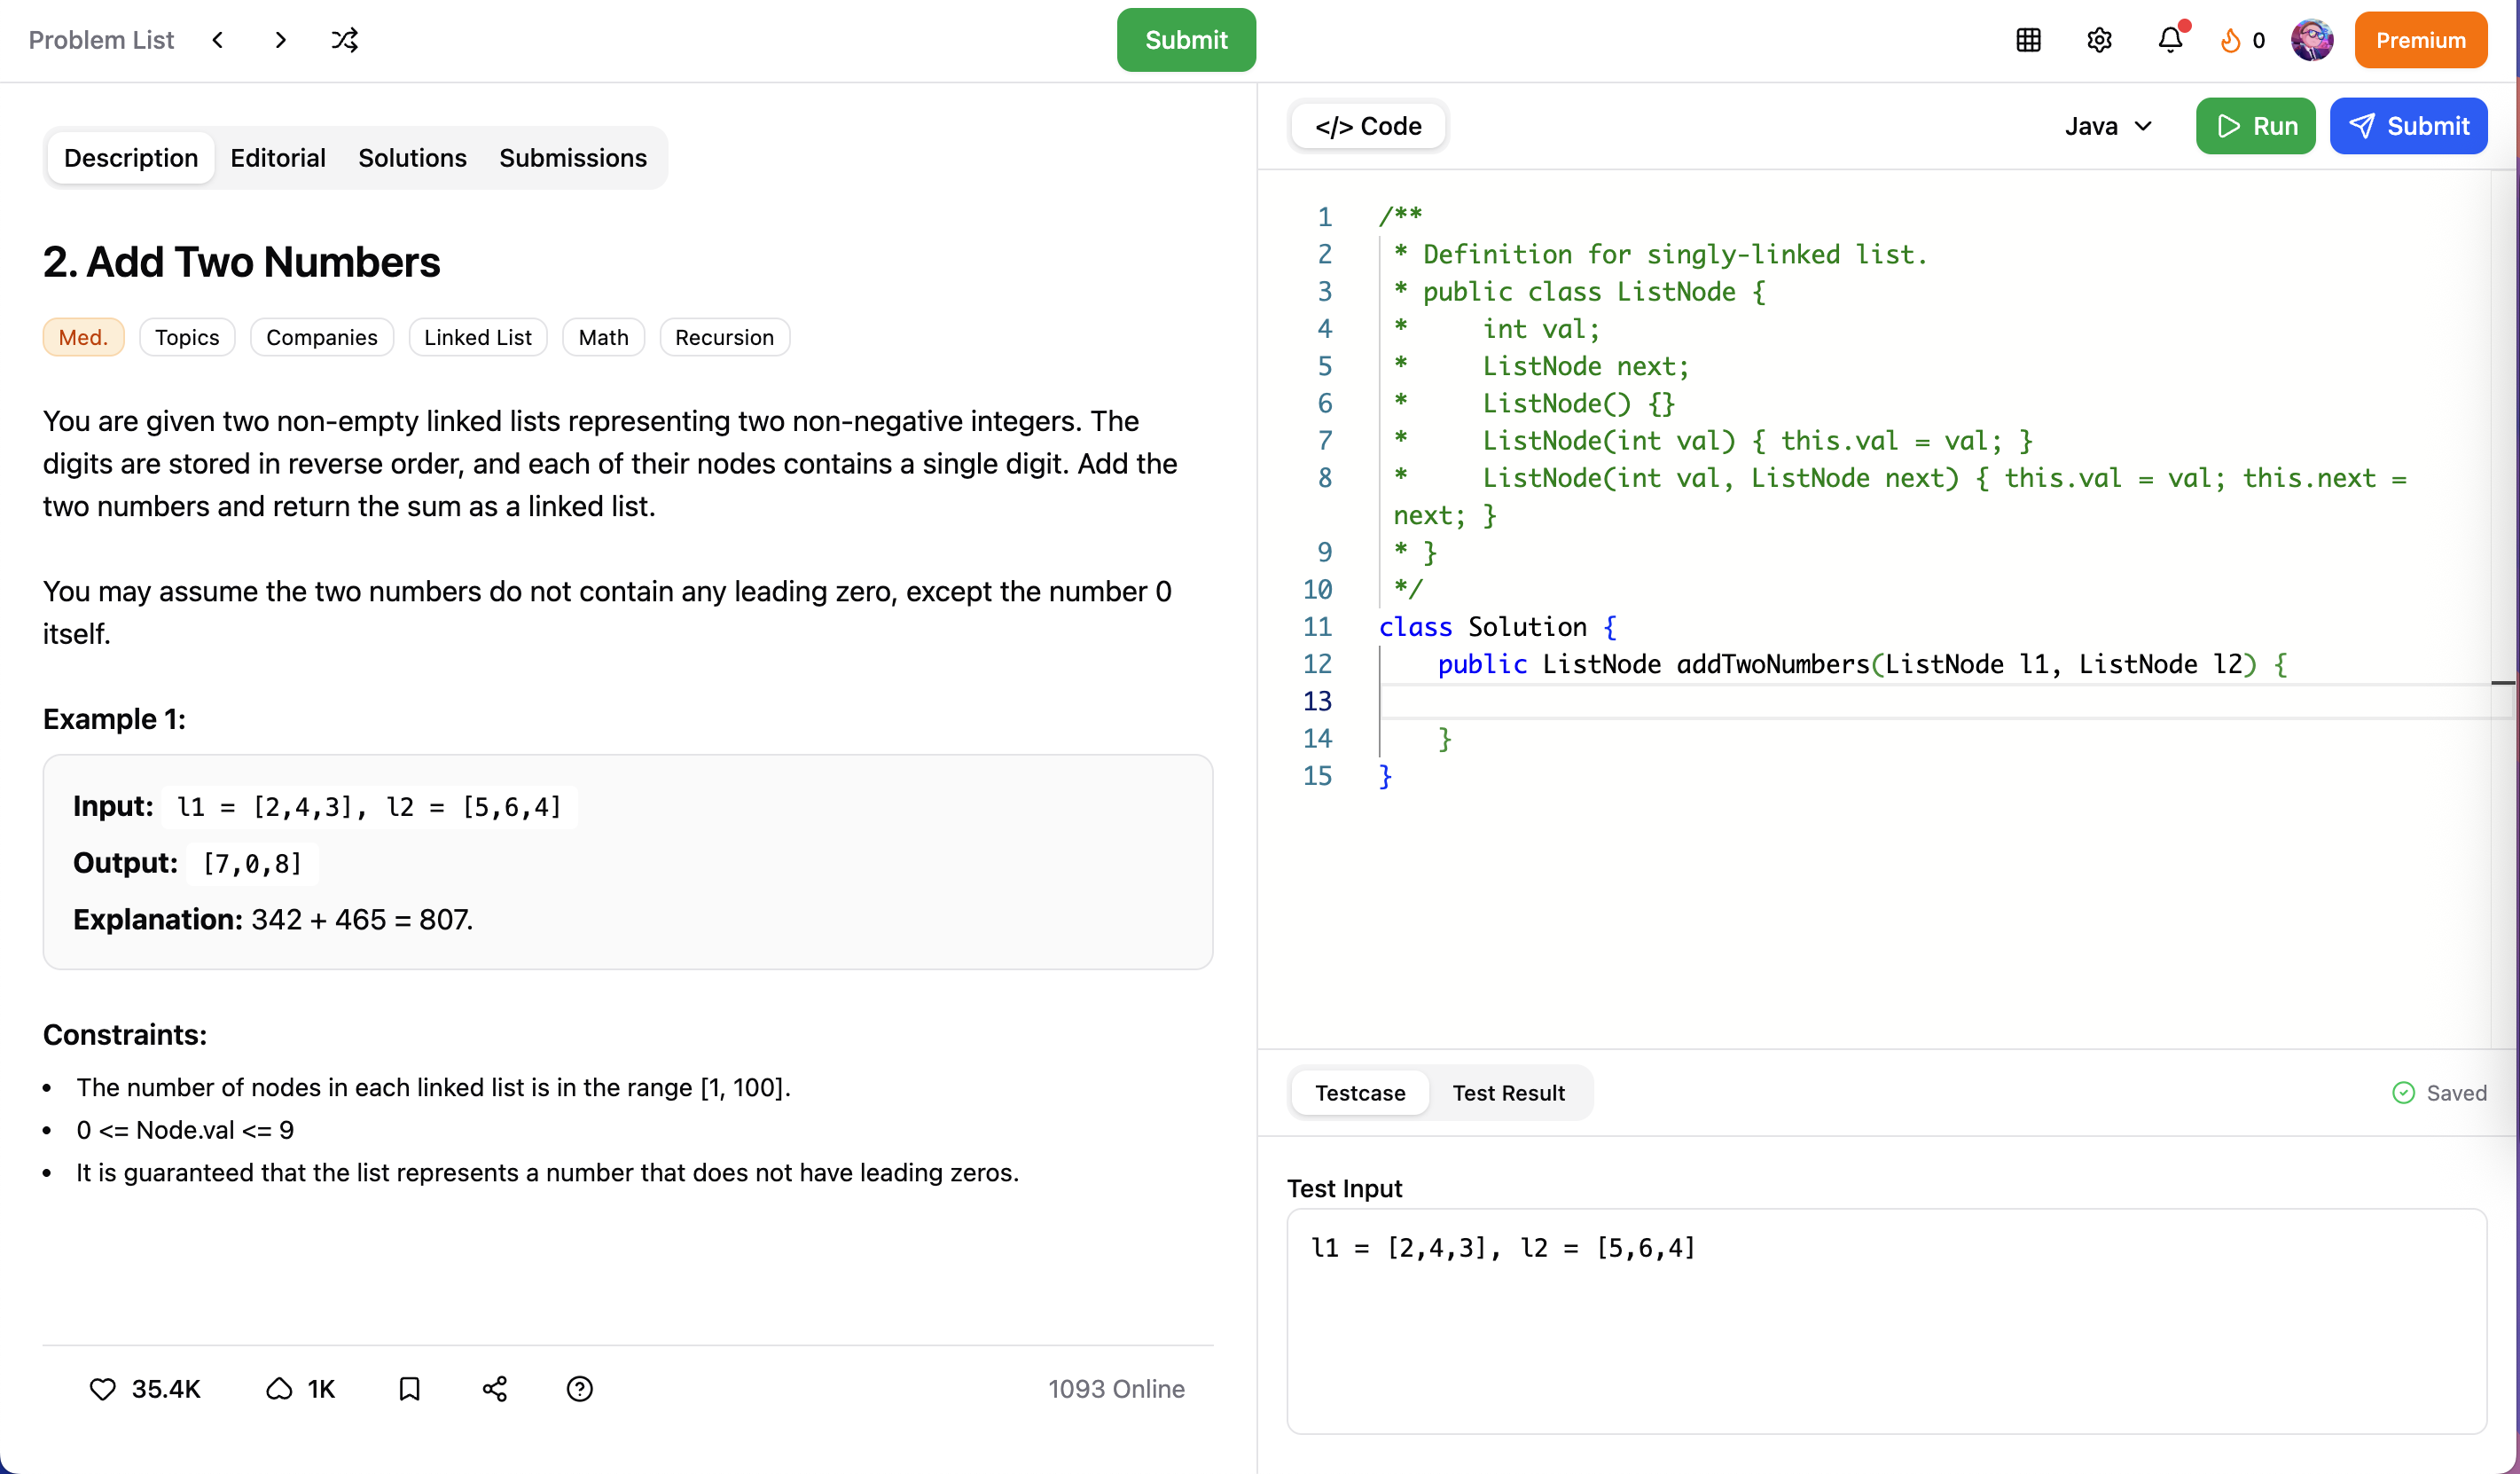
\includegraphics[width=1\textwidth]{Contents/Chapter 4/Mockup Design/Primary User/problem_detail.png}
    \vspace{0.6cm}
    \caption{Problem Detail page}
\end{figure}


\subsubsection*{Discussion}

Beside solving problems, primary user can access the Discussion feature from the main navigation menu after logging in. The Discussion feature allows users to engage in conversations related to coding problems, share insights, ask questions, and collaborate with other users.

\begin{figure}[H]
    \centering
    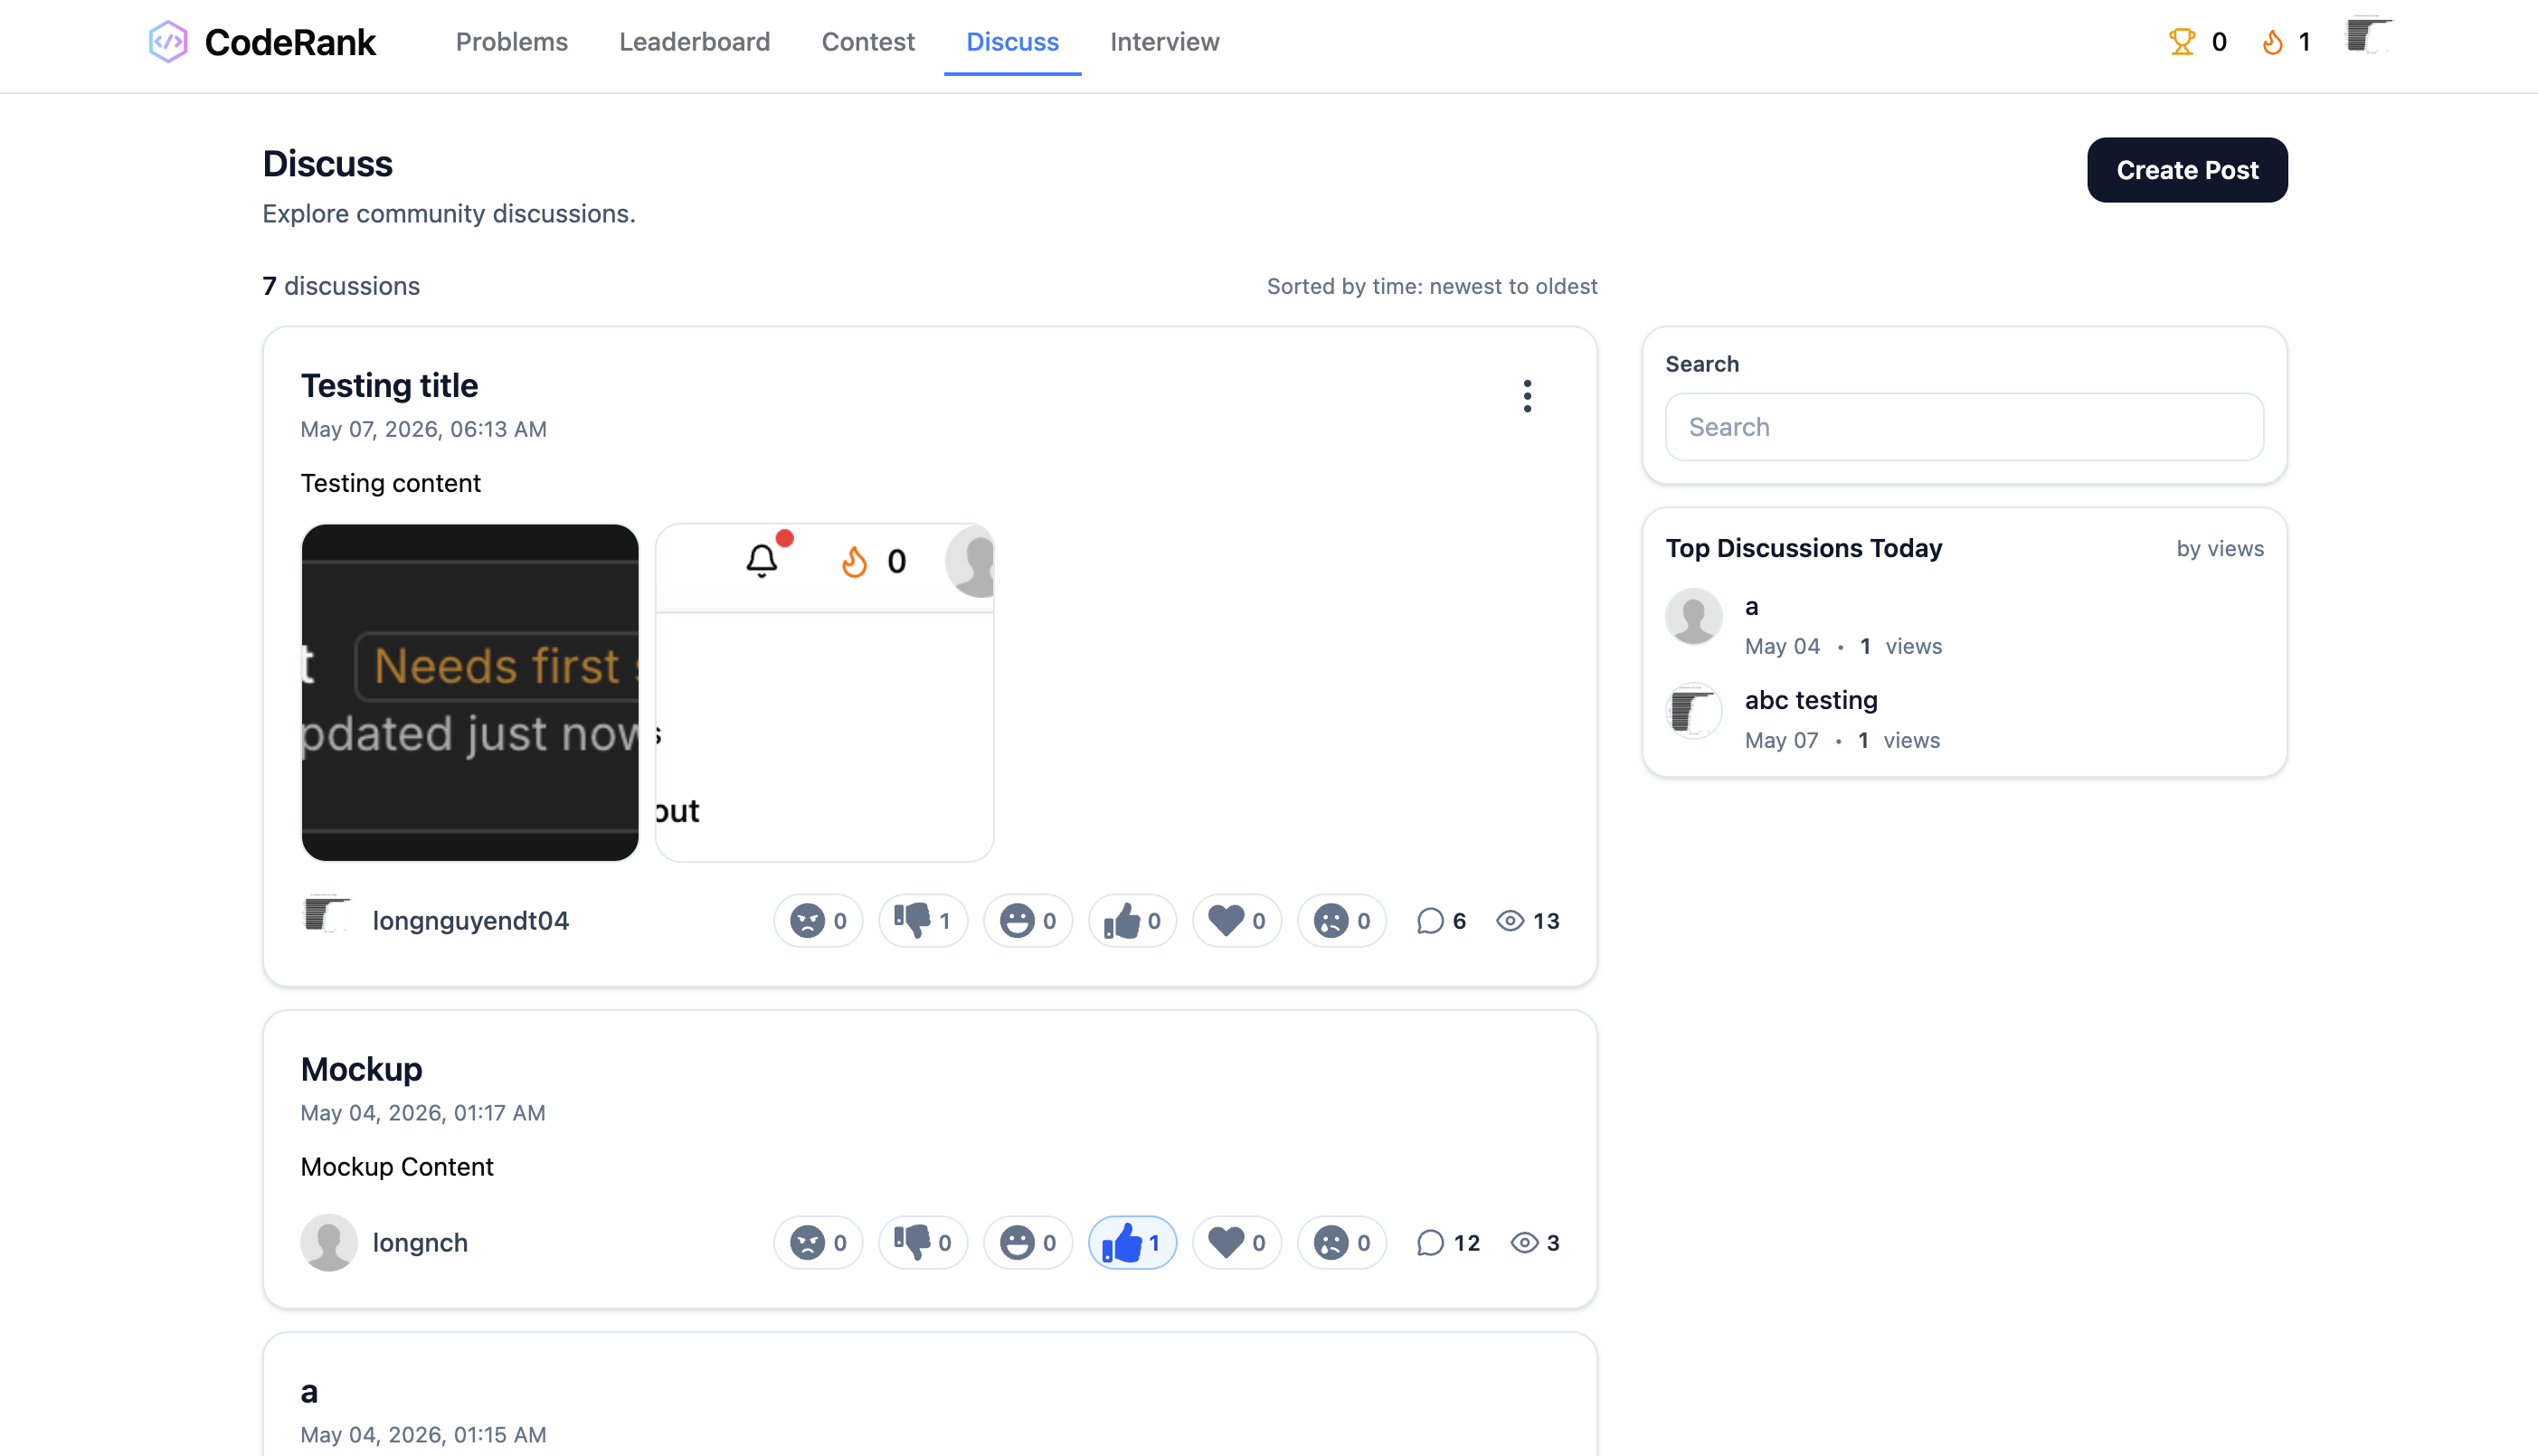
\includegraphics[width=1\textwidth]{Contents/Chapter 4/Mockup Design/Primary User/discussion-1.png}
    \vspace{0.6cm}
    \caption{Discussion List}
\end{figure}

In order to join a discussion, the user can select a specific discussion thread from the Discussion List. This will take them to the Discussion Detail page, where they can view all messages within that thread and participate in the conversation by posting their own messages.
\begin{figure}[H]
    \centering
    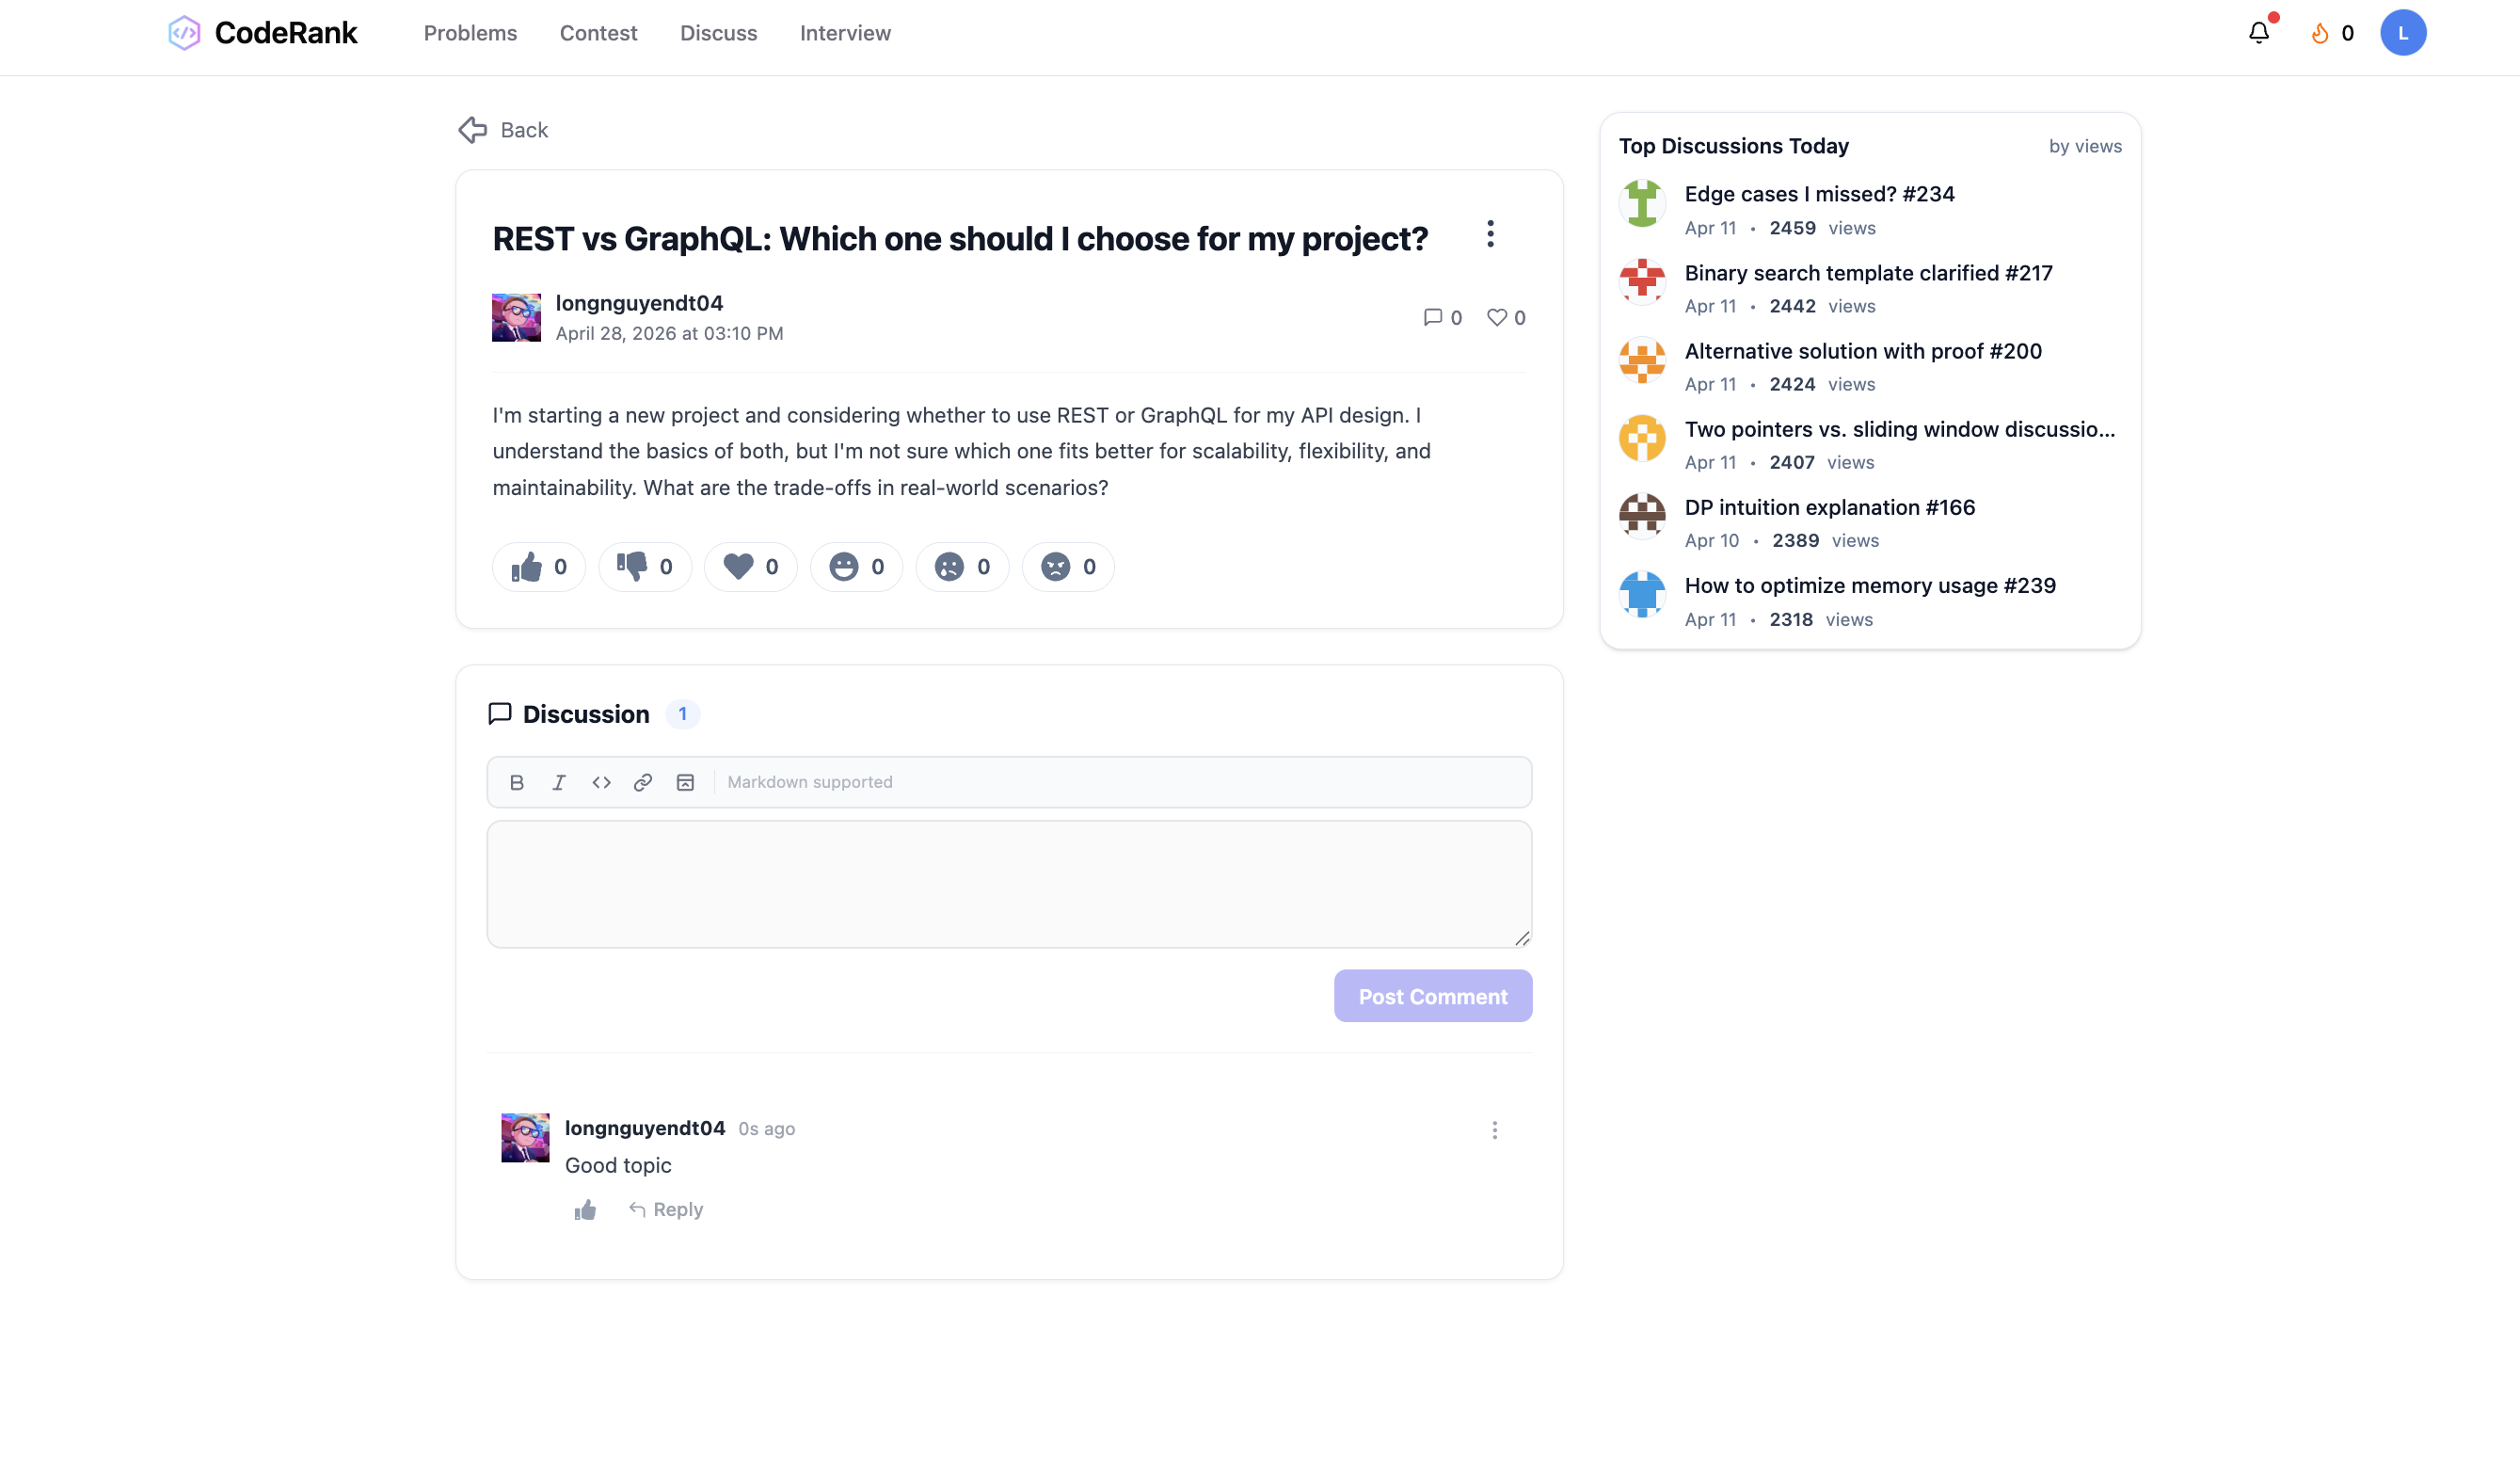
\includegraphics[width=1\textwidth]{Contents/Chapter 4/Mockup Design/Primary User/discussion-3.png}
    \vspace{0.6cm}
    \caption{Discussion Detail}
\end{figure}

To create a new discussion thread, the user can click in the button \textbf{Create} in the discussion list page. Here, they can enter a title, choose topic, tags, and write the initial message to start the discussion.

\begin{figure}[H]
    \centering
    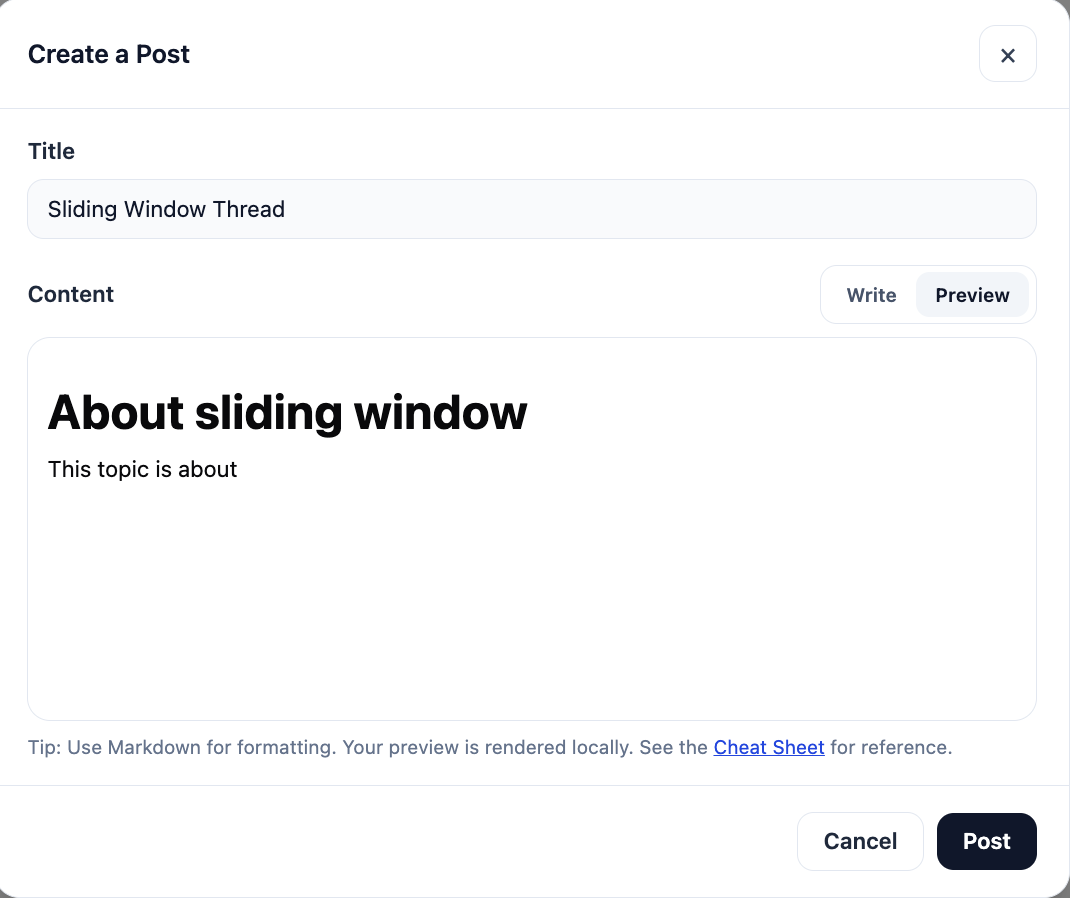
\includegraphics[width=1\textwidth]{Contents/Chapter 4/Mockup Design/Primary User/discussion-2.png}
    \vspace{0.6cm}
    \caption{Create Discussion}
\end{figure}

\subsubsection*{Contest Participation}

Primary users can participate in coding contests hosted on the platform by navigating to the Contest List page from the main navigation menu. This page displays a list of upcoming and ongoing contests, along with relevant details such as contest name, start time, end time, and duration.
\begin{figure}[H]
    \centering
    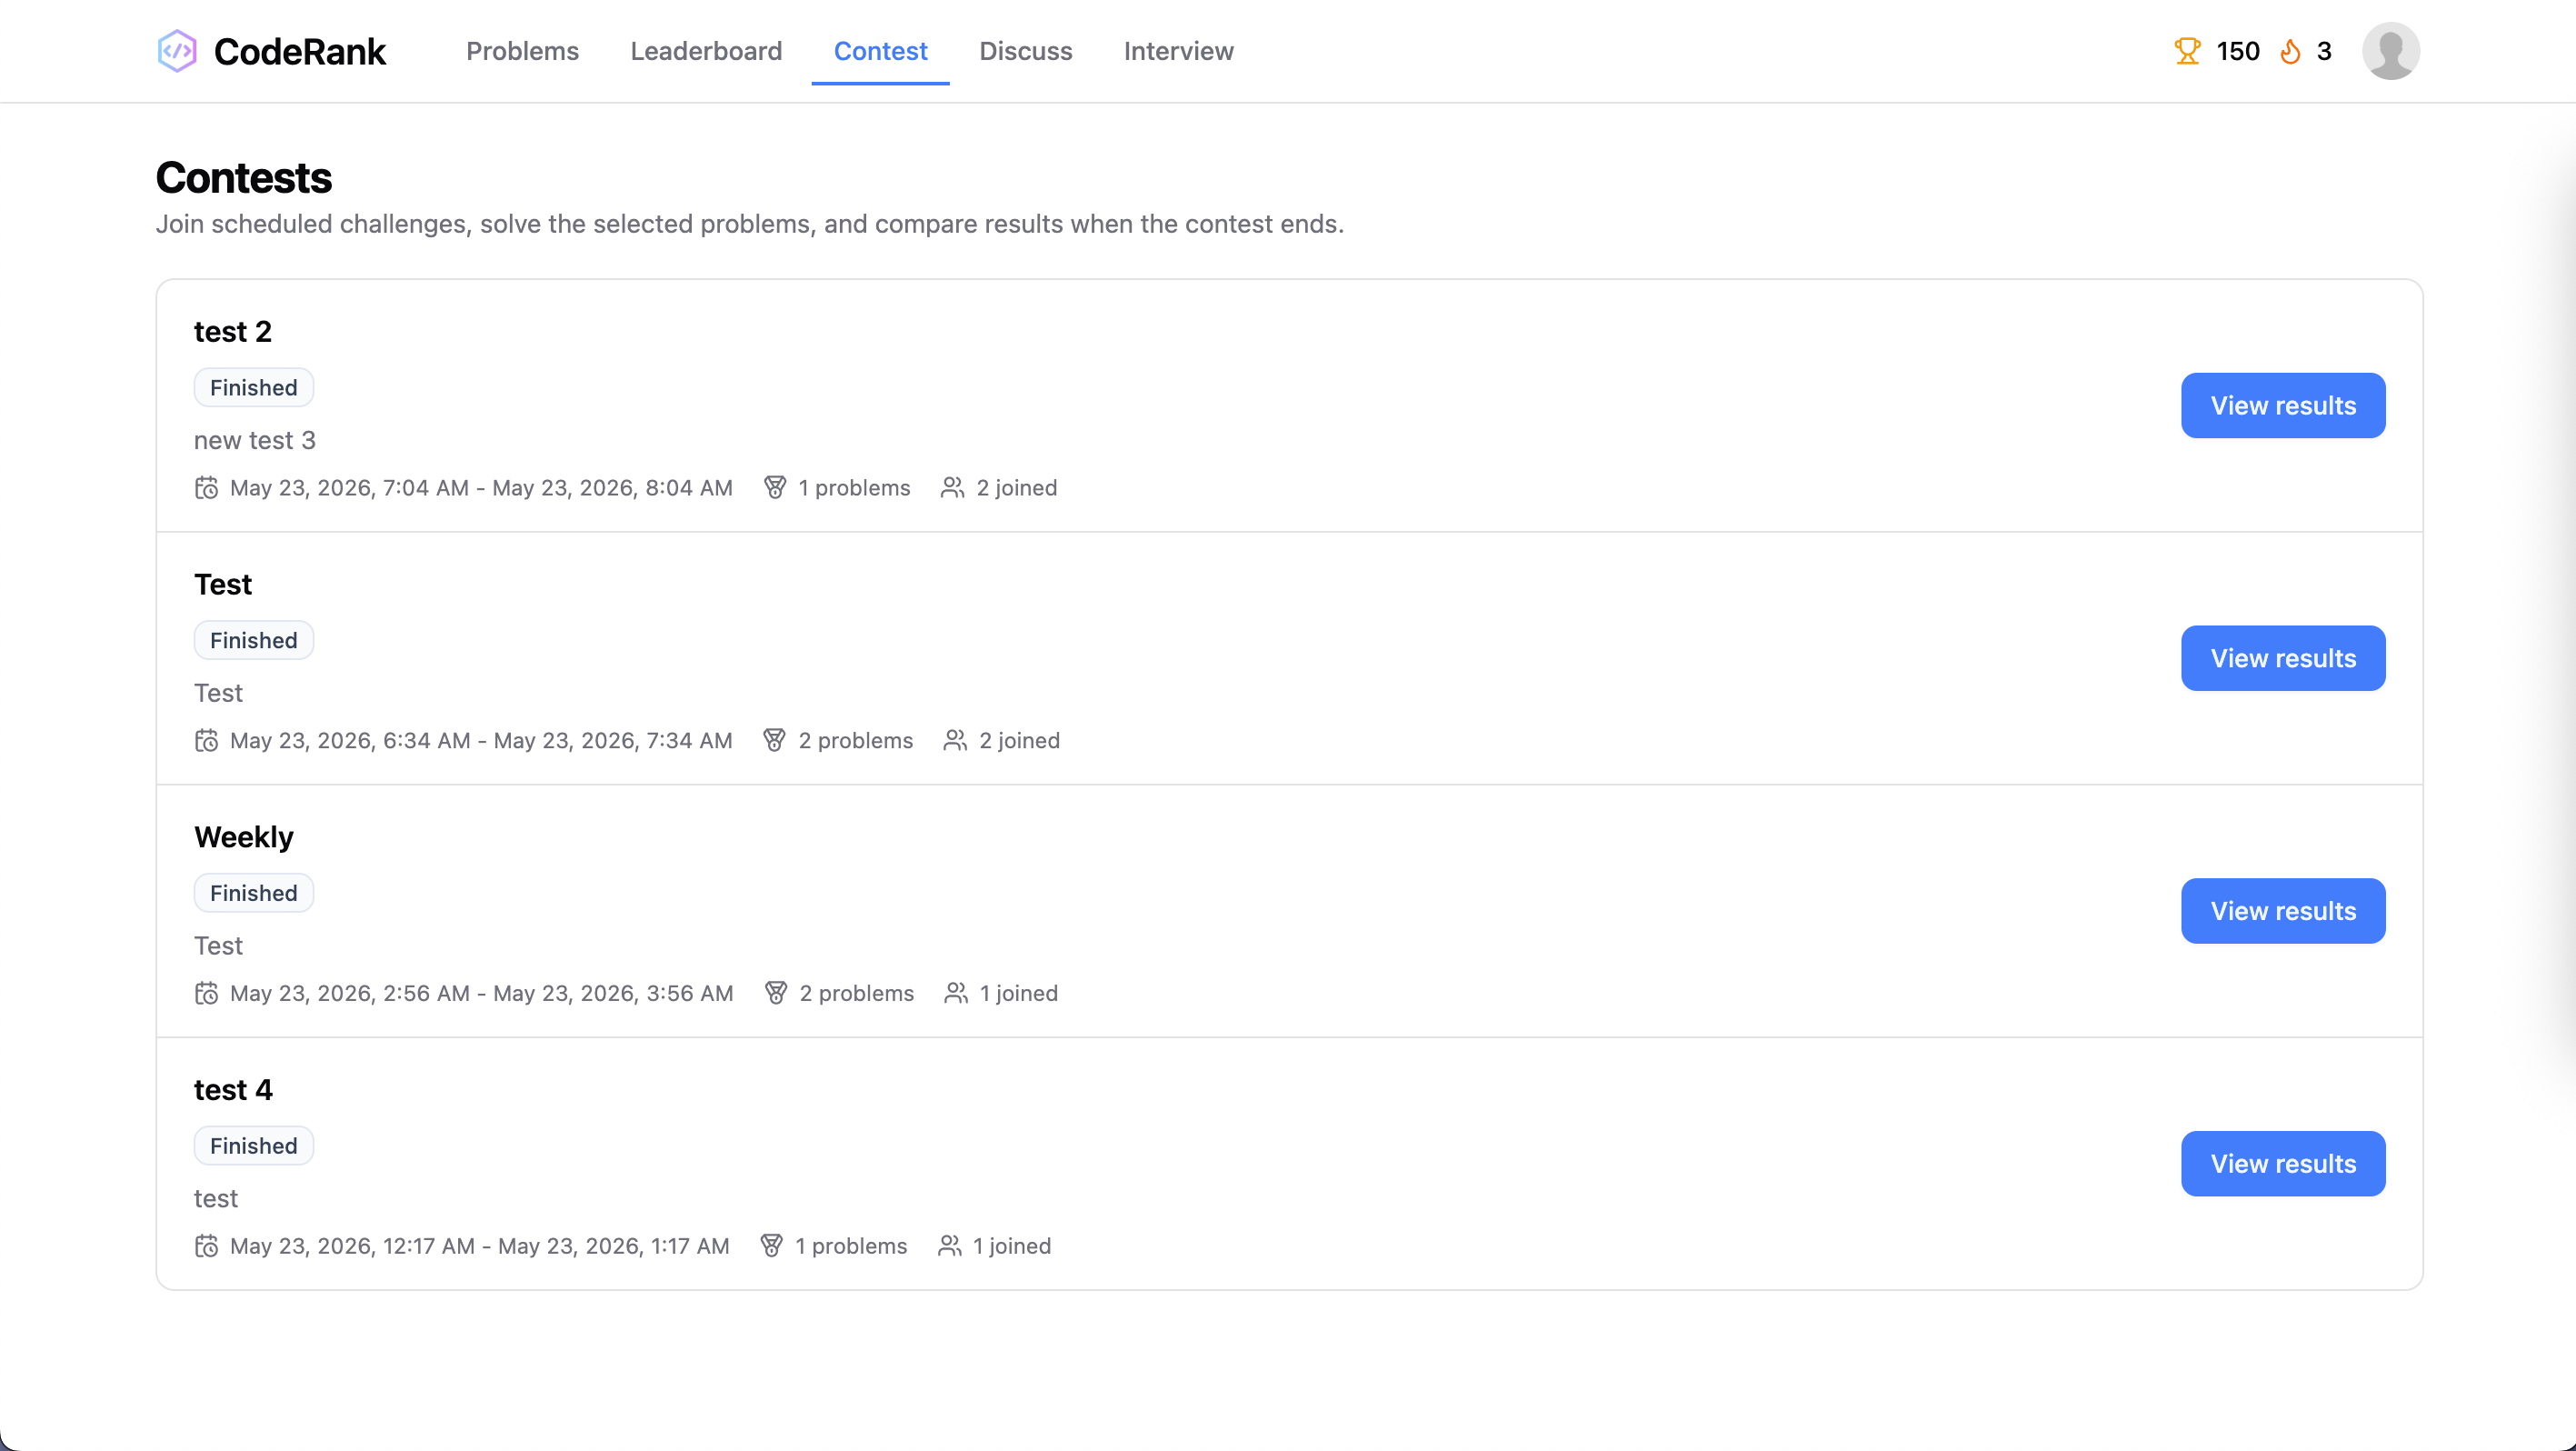
\includegraphics[width=1\textwidth]{Contents/Chapter 4/Mockup Design/Primary User/contest-1.png}
    \vspace{0.6cm}
    \caption{Contest List}
\end{figure}

In order to view the details of a specific contest, the user can click on the contest name in the Contest List. This will take them to the Contest Detail page, where they can see the information about the contest, including the list of problems included in the contest.
\begin{figure}[H]
    \centering
    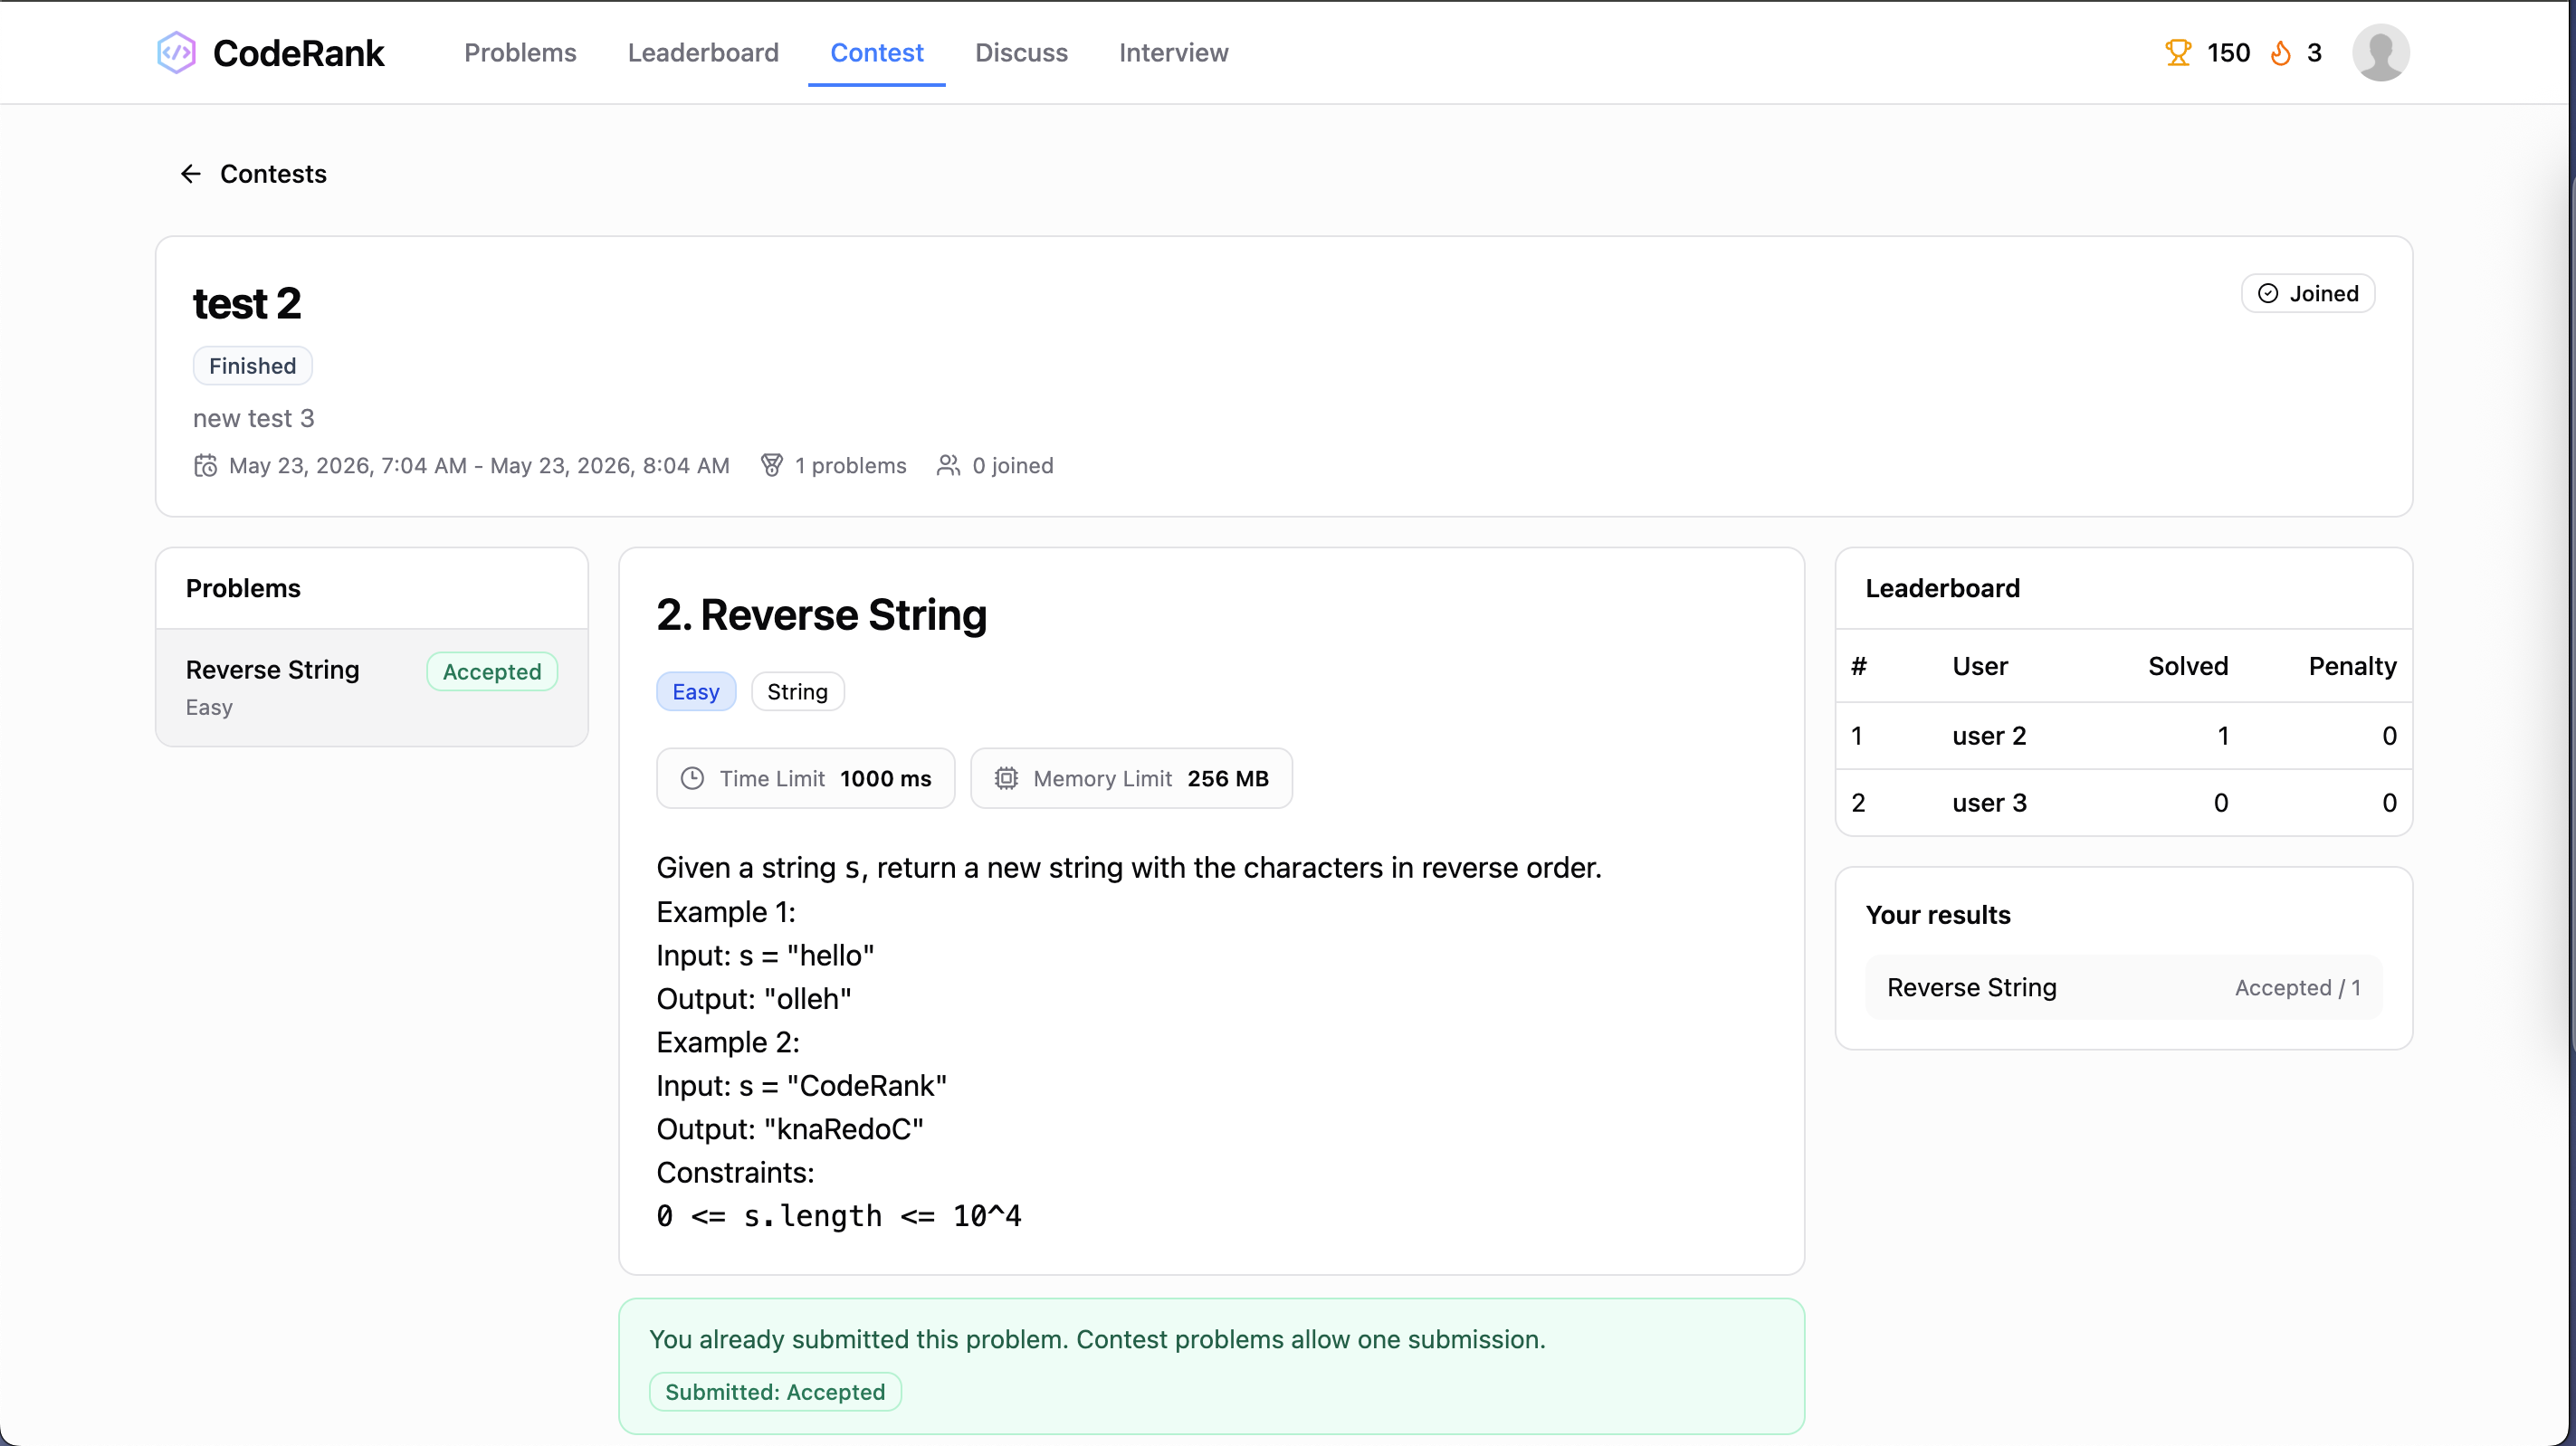
\includegraphics[width=1\textwidth]{Contents/Chapter 4/Mockup Design/Primary User/contest-2.png}
    \vspace{0.6cm}
    \caption{Contest Detail}
\end{figure}


In order to create a custom contest, moderator can go to the Contest monitor page. Here, they can enter the contest name, select problems to include in the contest, set the start and end time, and define other contest settings.
\begin{figure}[H]
    \centering
    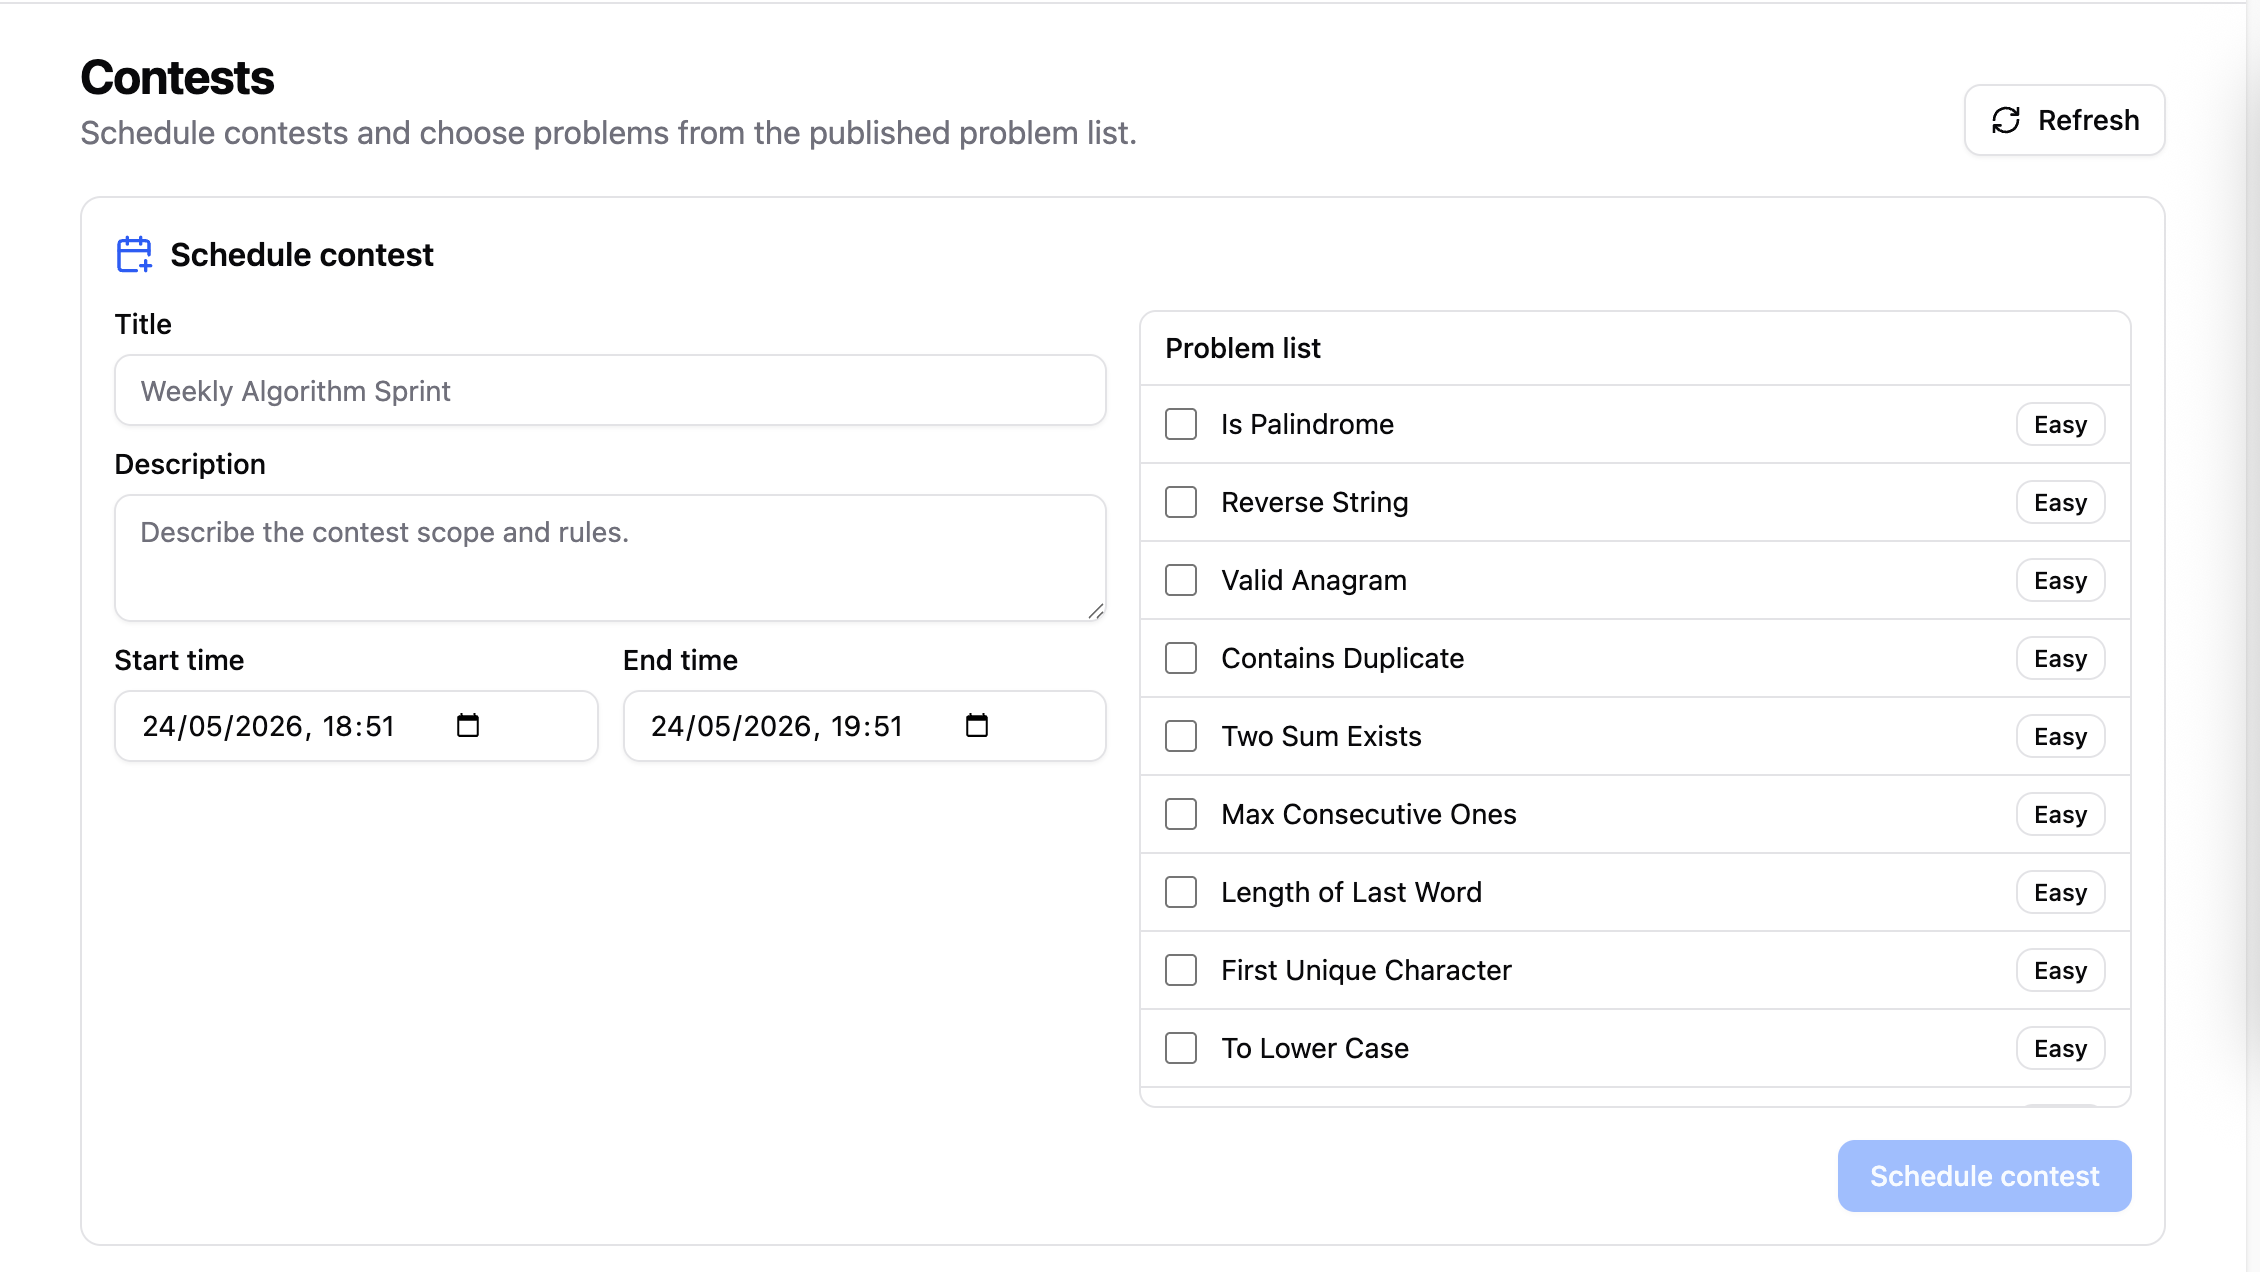
\includegraphics[width=1\textwidth]{Contents/Chapter 4/Mockup Design/Primary User/contest-3.png}
    \vspace{0.6cm}
    \caption{Contest Creation}
\end{figure}

\subsubsection*{Interview Preparation}
Primary users can access the Interview Preparation feature from the main navigation menu. The Interview Preparation feature provides users with a curated list of coding problems and resources specifically designed to help them prepare for technical interviews. In the Interview Preparation page, there will be a conversation history section on the left side, displaying a list of previous interview preparation sessions. Users can select a session to view the details and continue their preparation or create a new session by clicking the \textbf{New Conversation} button.
\begin{figure}[H]
    \centering
    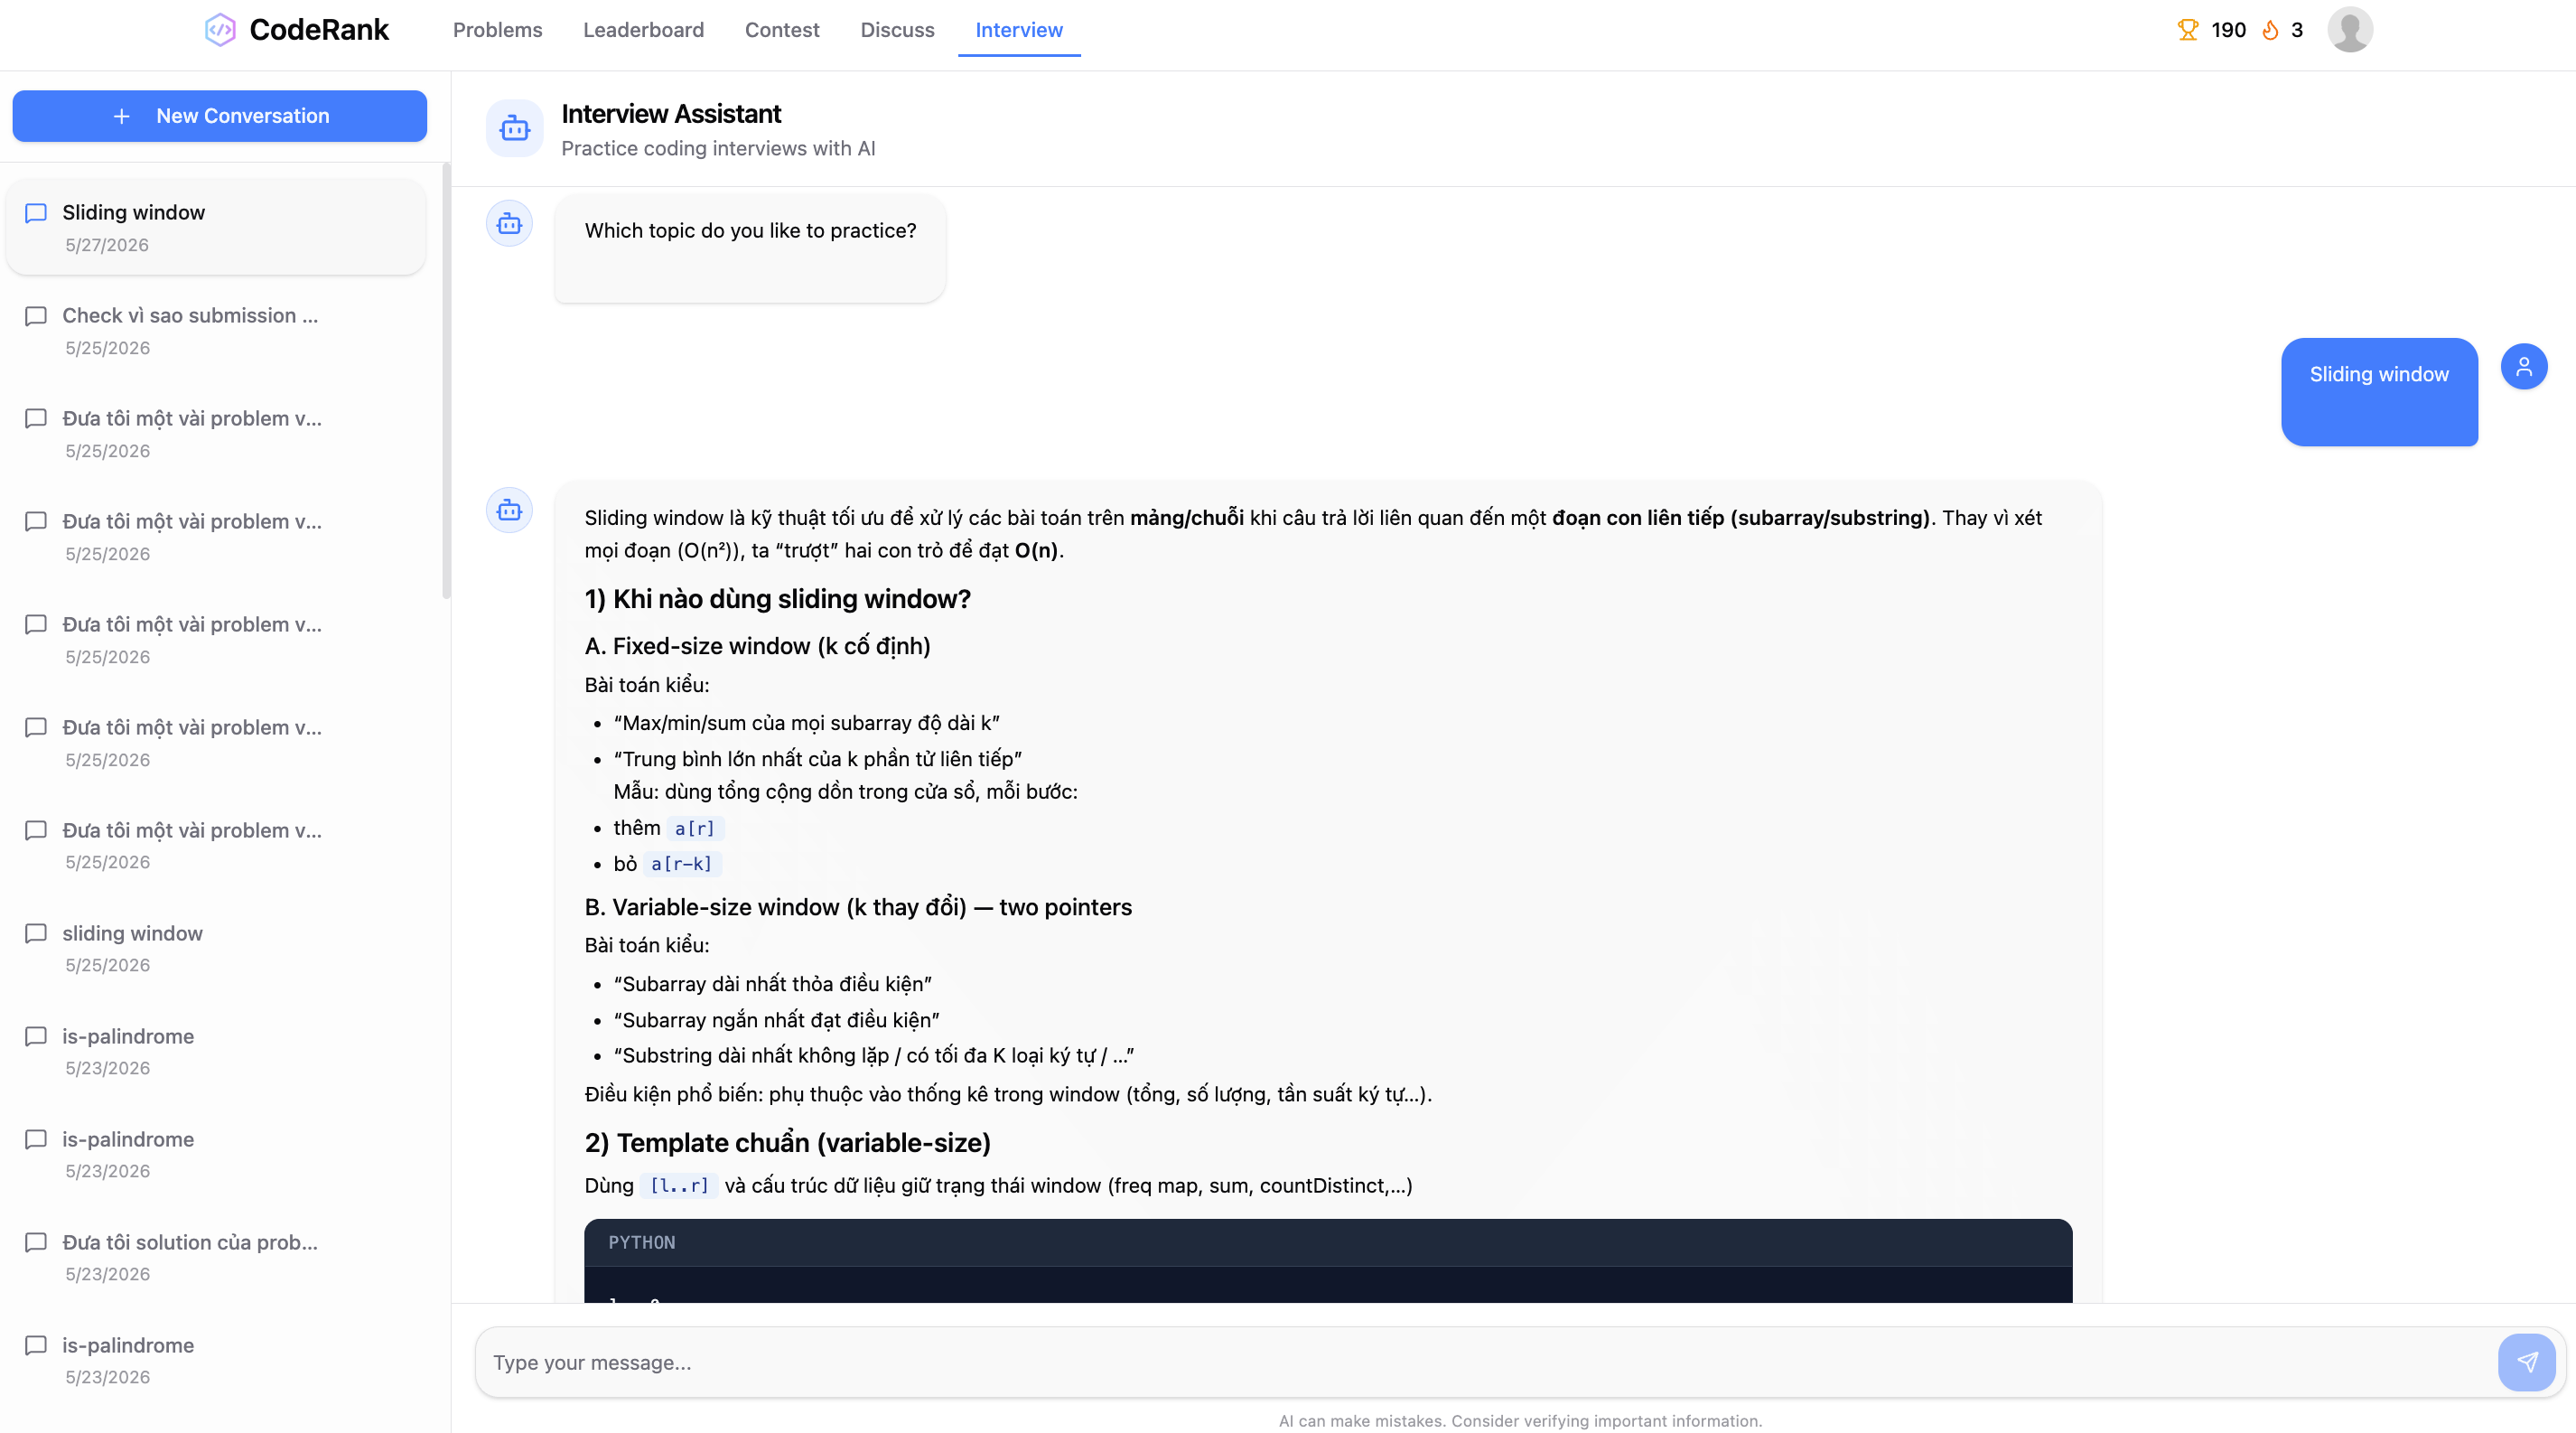
\includegraphics[width=1\textwidth]{Contents/Chapter 4/Mockup Design/Primary User/interview-1.png}
    \vspace{0.6cm}
    \caption{Interview Preparation Page}
\end{figure}

\subsection{Moderator/Admin flow}

After logging in as a Moderator/Admin, the user will be directed to the Moderator/Superadmin Dashboard. This dashboard provides an overview of key metrics and functionalities available to moderators and administrators, allowing them to manage the platform effectively.
\begin{figure}[H]
    \centering
    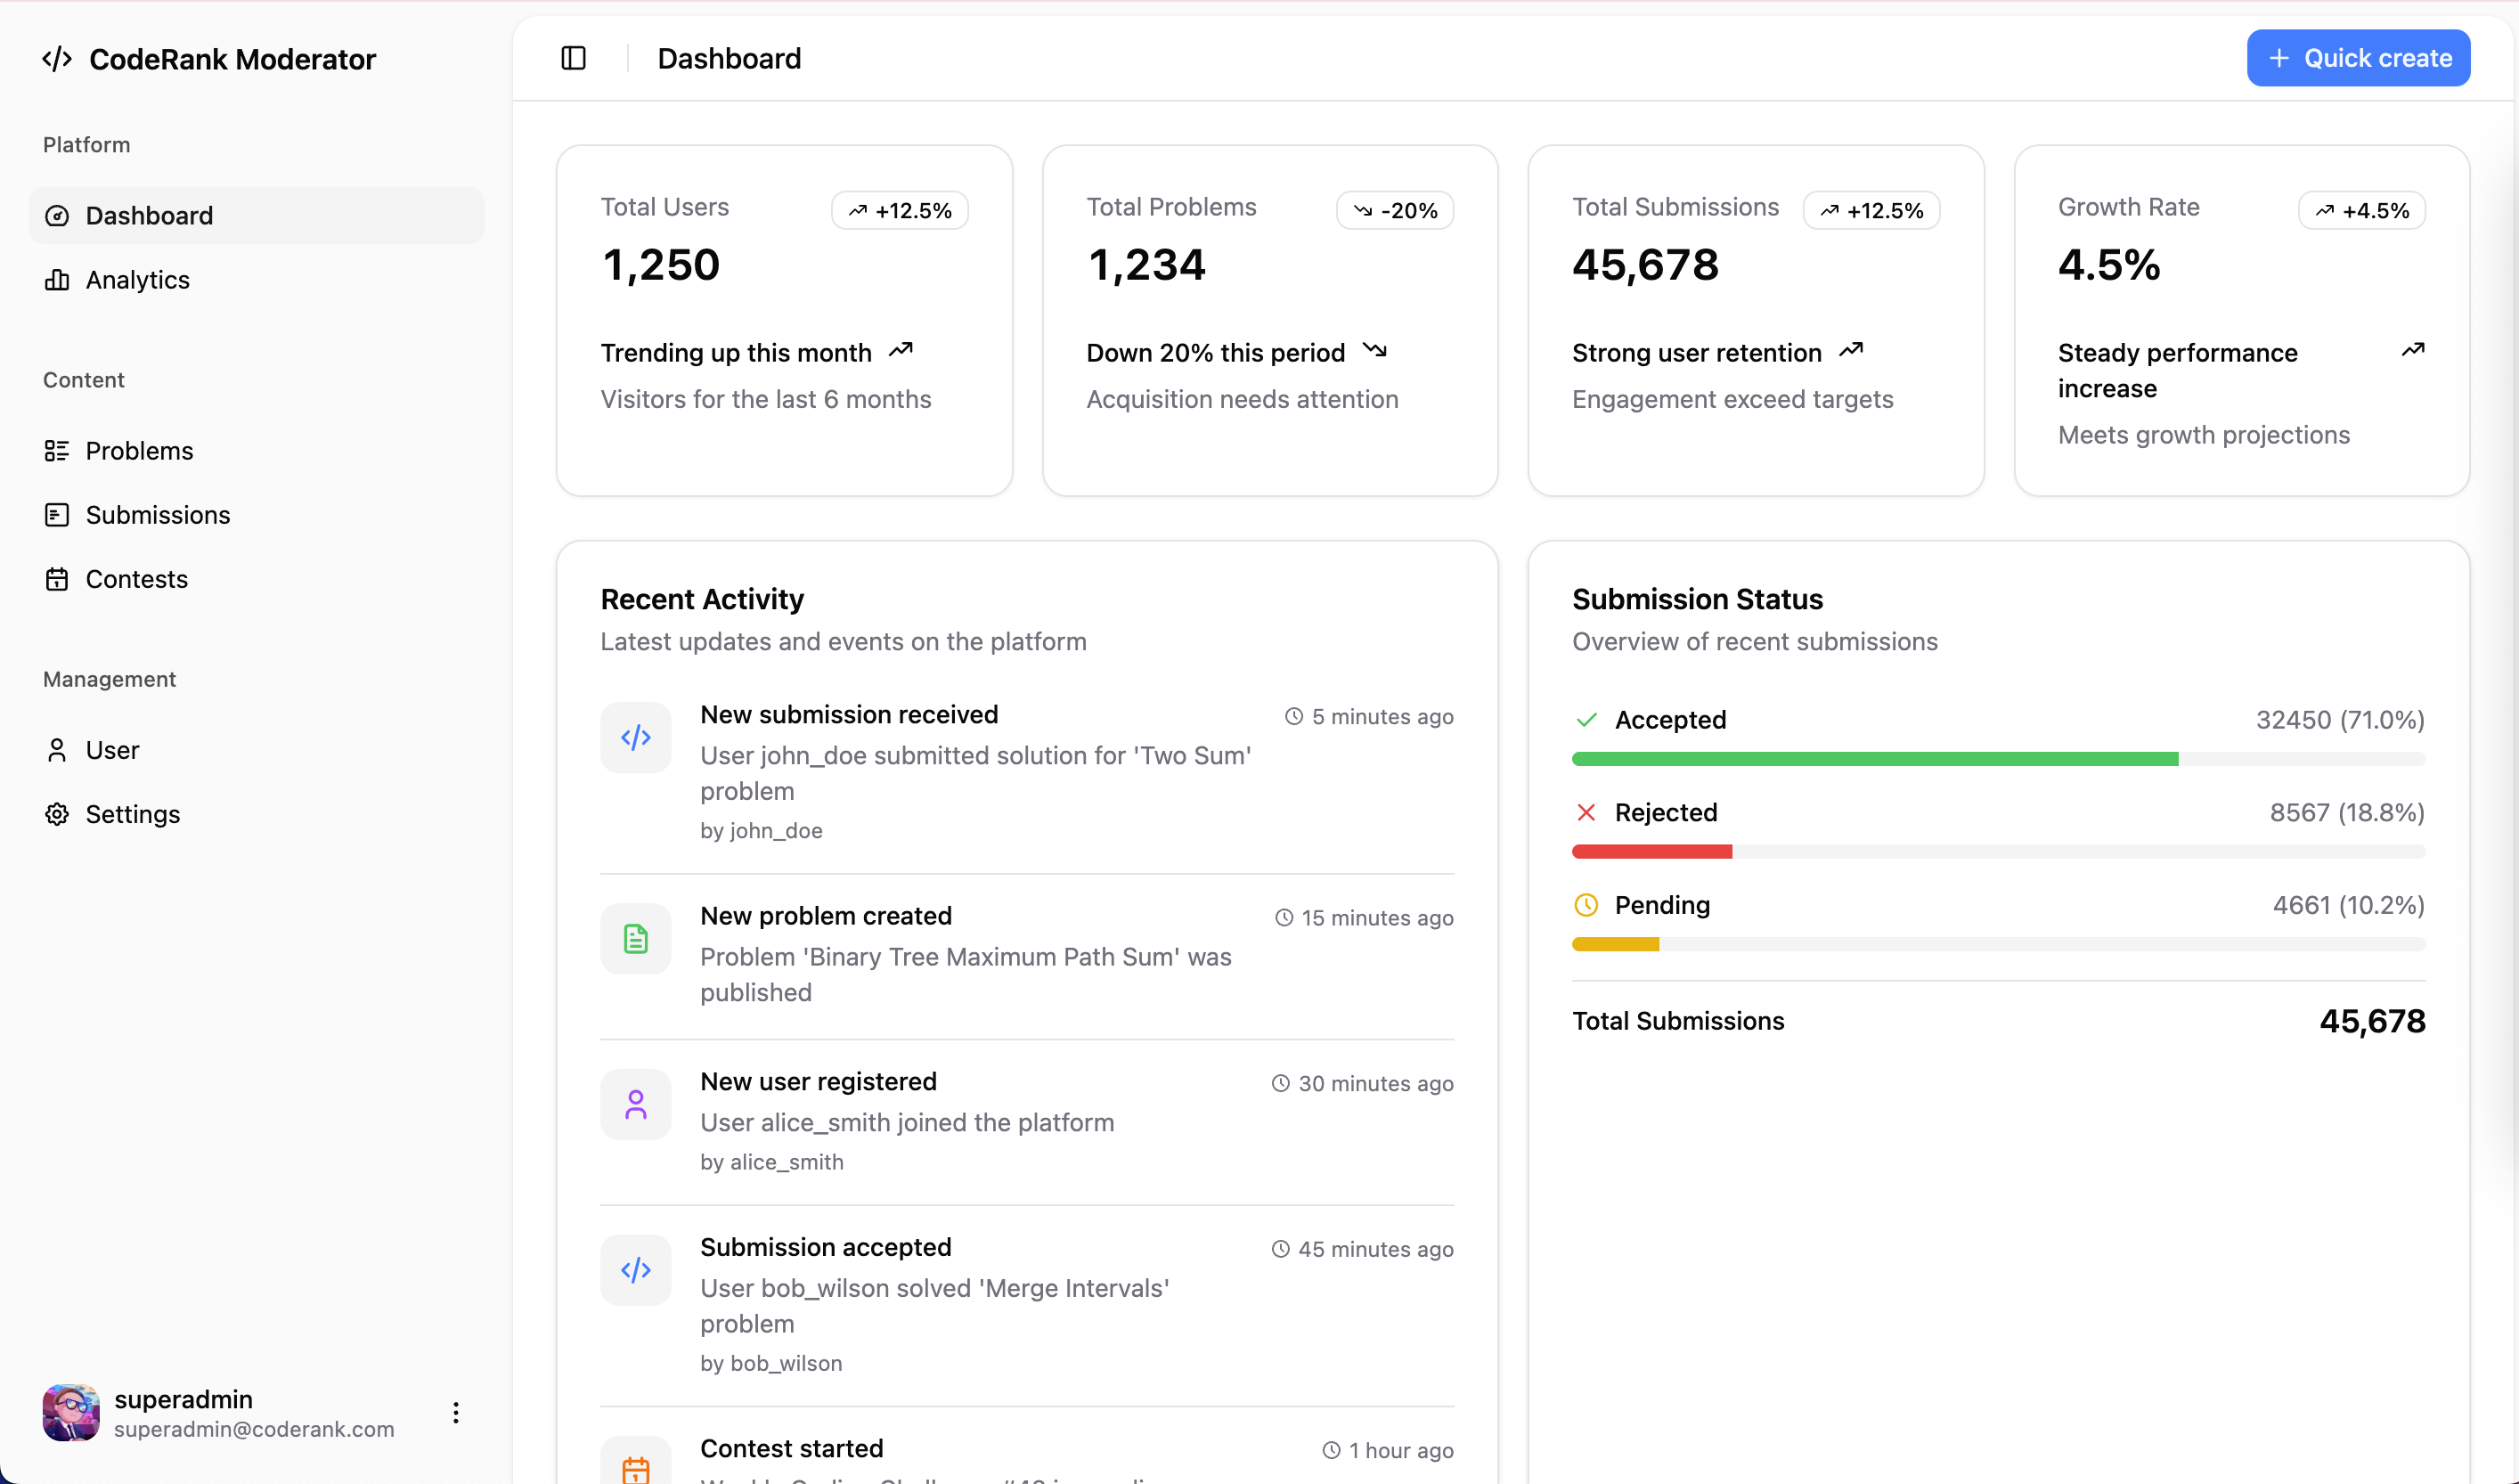
\includegraphics[width=1\textwidth]{Contents/Chapter 4/Mockup Design/Admin/admin-1.png}
    \vspace{0.6cm}
    \caption{Moderator Dashboard}
\end{figure}

The Moderator/Admin dashboard also provides centralized management interfaces for major platform resources. These interfaces allow privileged users to inspect system data, update operational content, and perform moderation actions from a consistent administrative workspace.

The Discussion Management interface displays all discussion threads available in the system. From this screen, Moderators/Admins can open a discussion detail page, review its comments, edit inappropriate content when necessary, or delete discussions and comments that violate platform policies.
\begin{figure}[H]
    \centering
    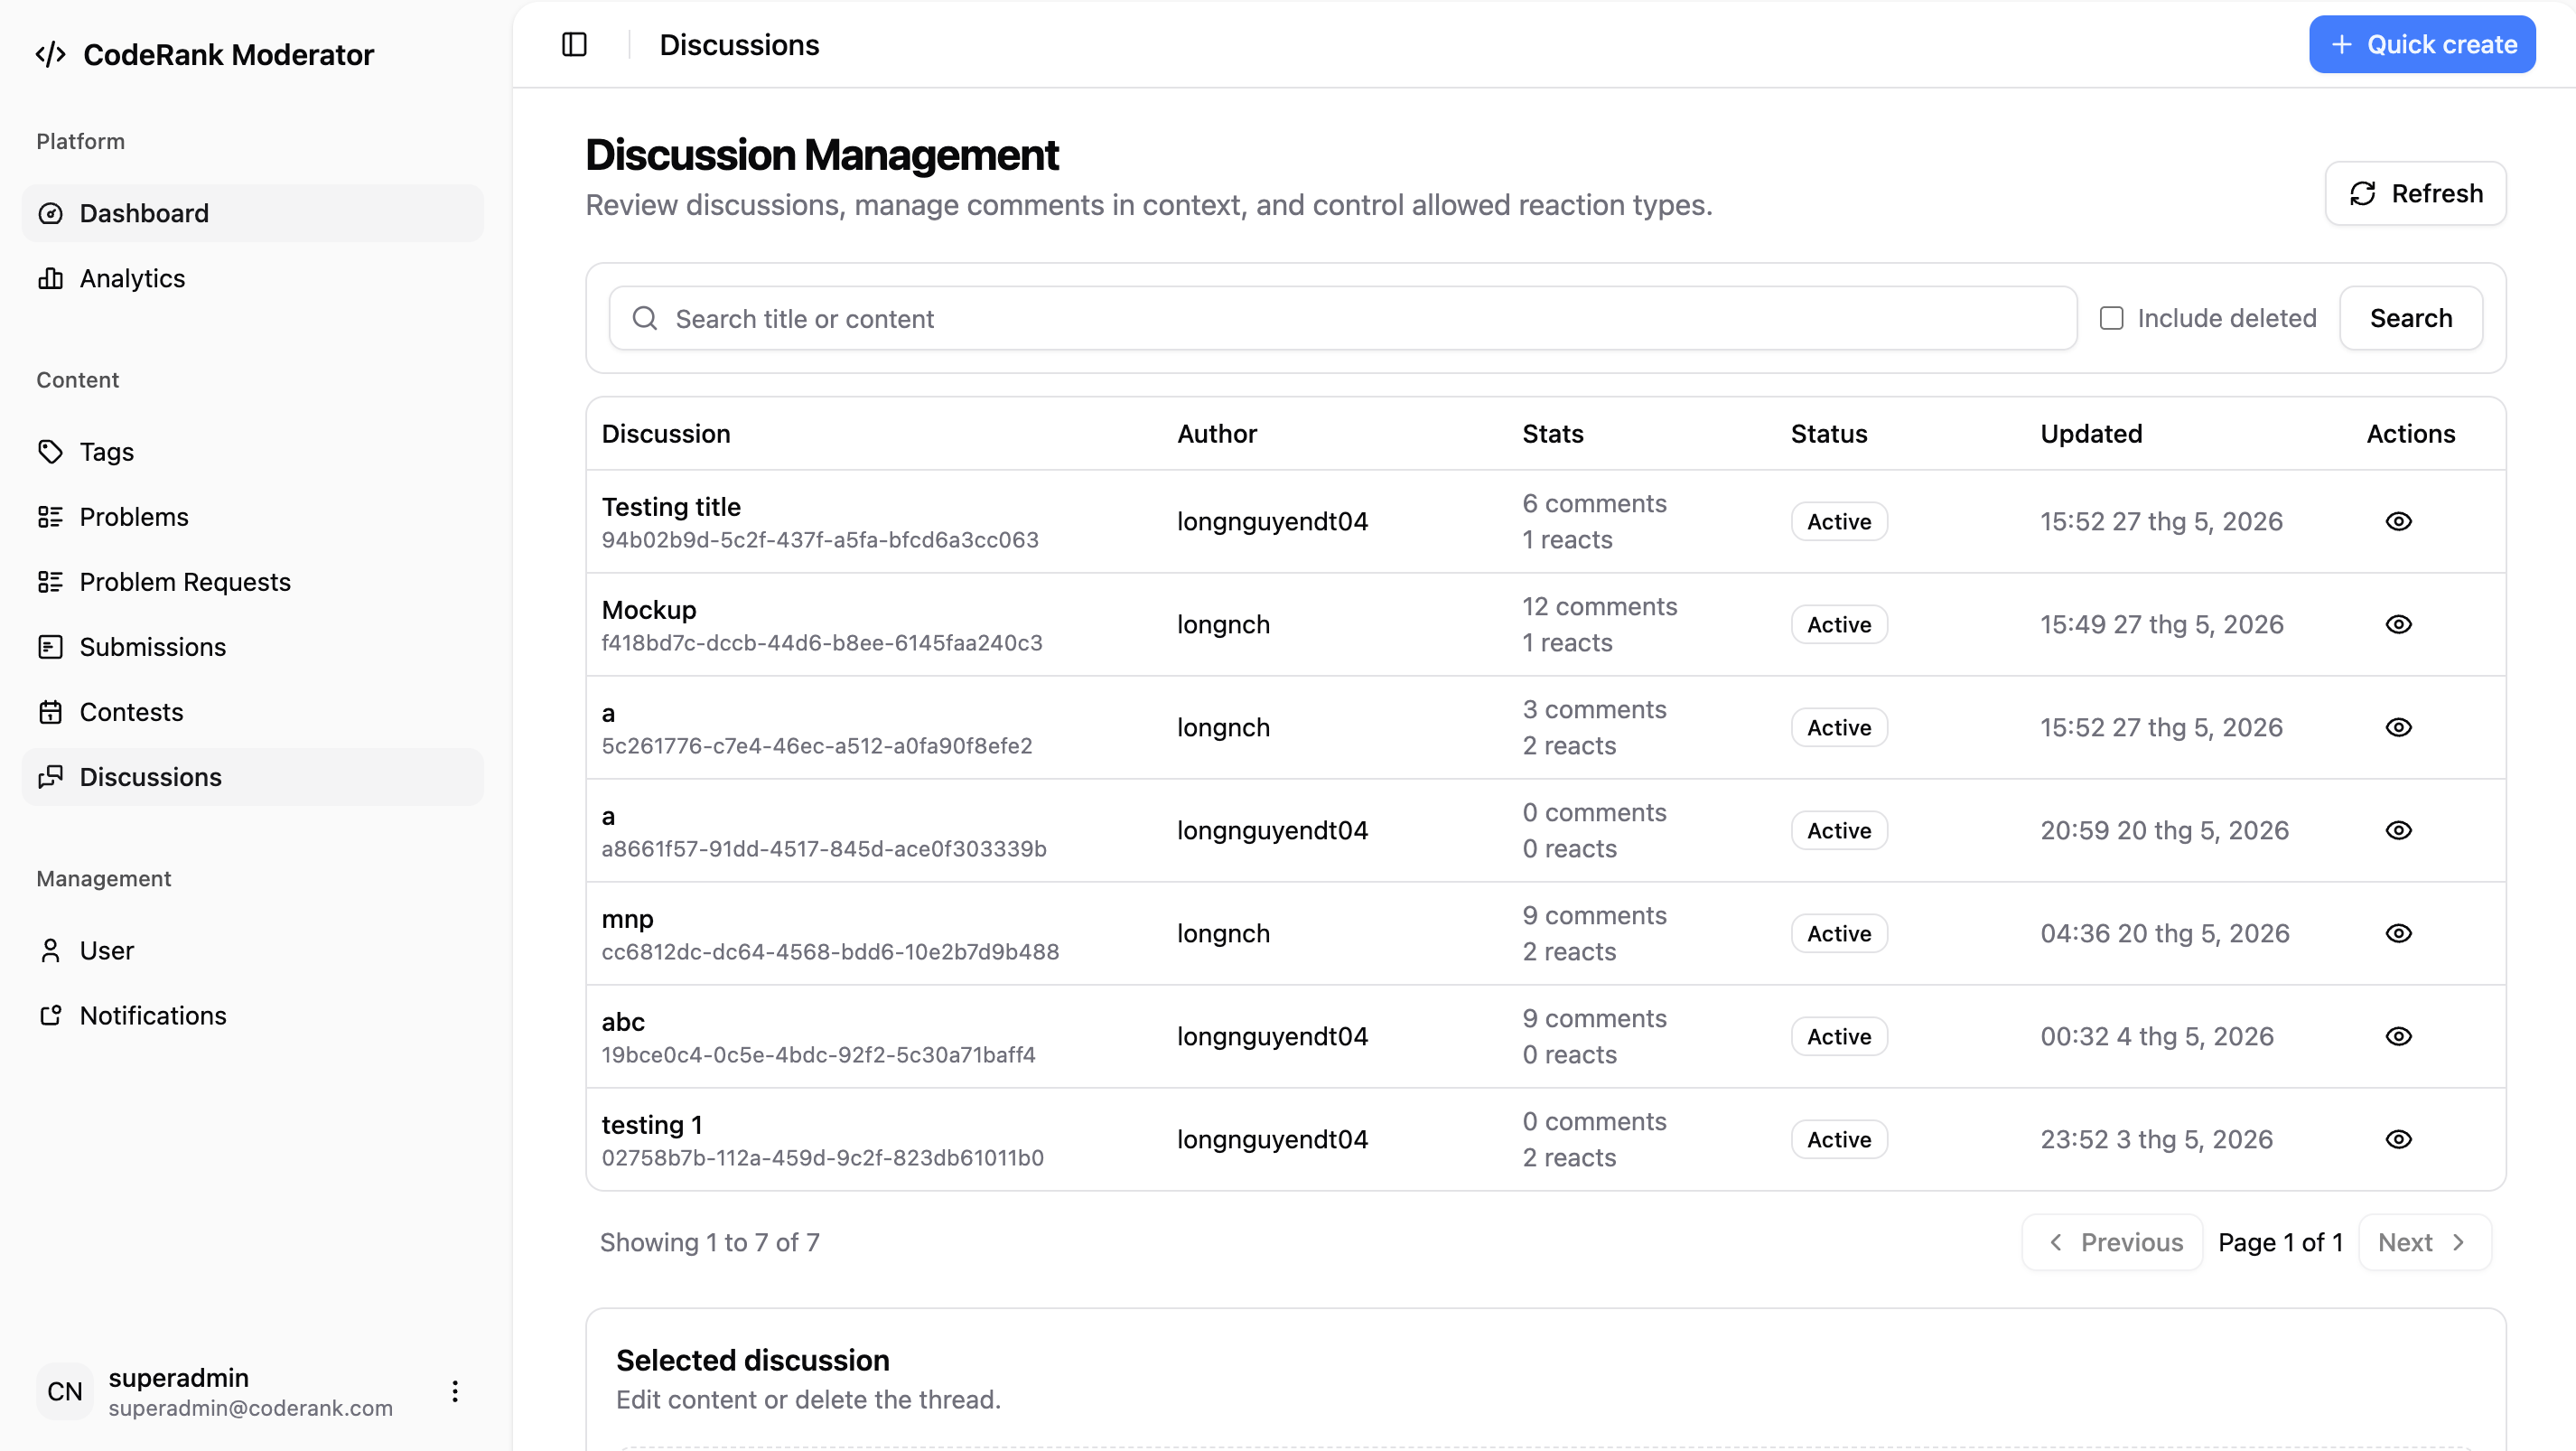
\includegraphics[width=1\textwidth]{Contents/Chapter 4/Mockup Design/Admin/discussion_management.png}
    \vspace{0.6cm}
    \caption{Discussion Management}
\end{figure}

The Contest Management interface supports the creation, editing, and maintenance of contest content. Moderators/Admins can configure contest information, update contest details, and manage contest-related content from a single administrative view.
\begin{figure}[H]
    \centering
    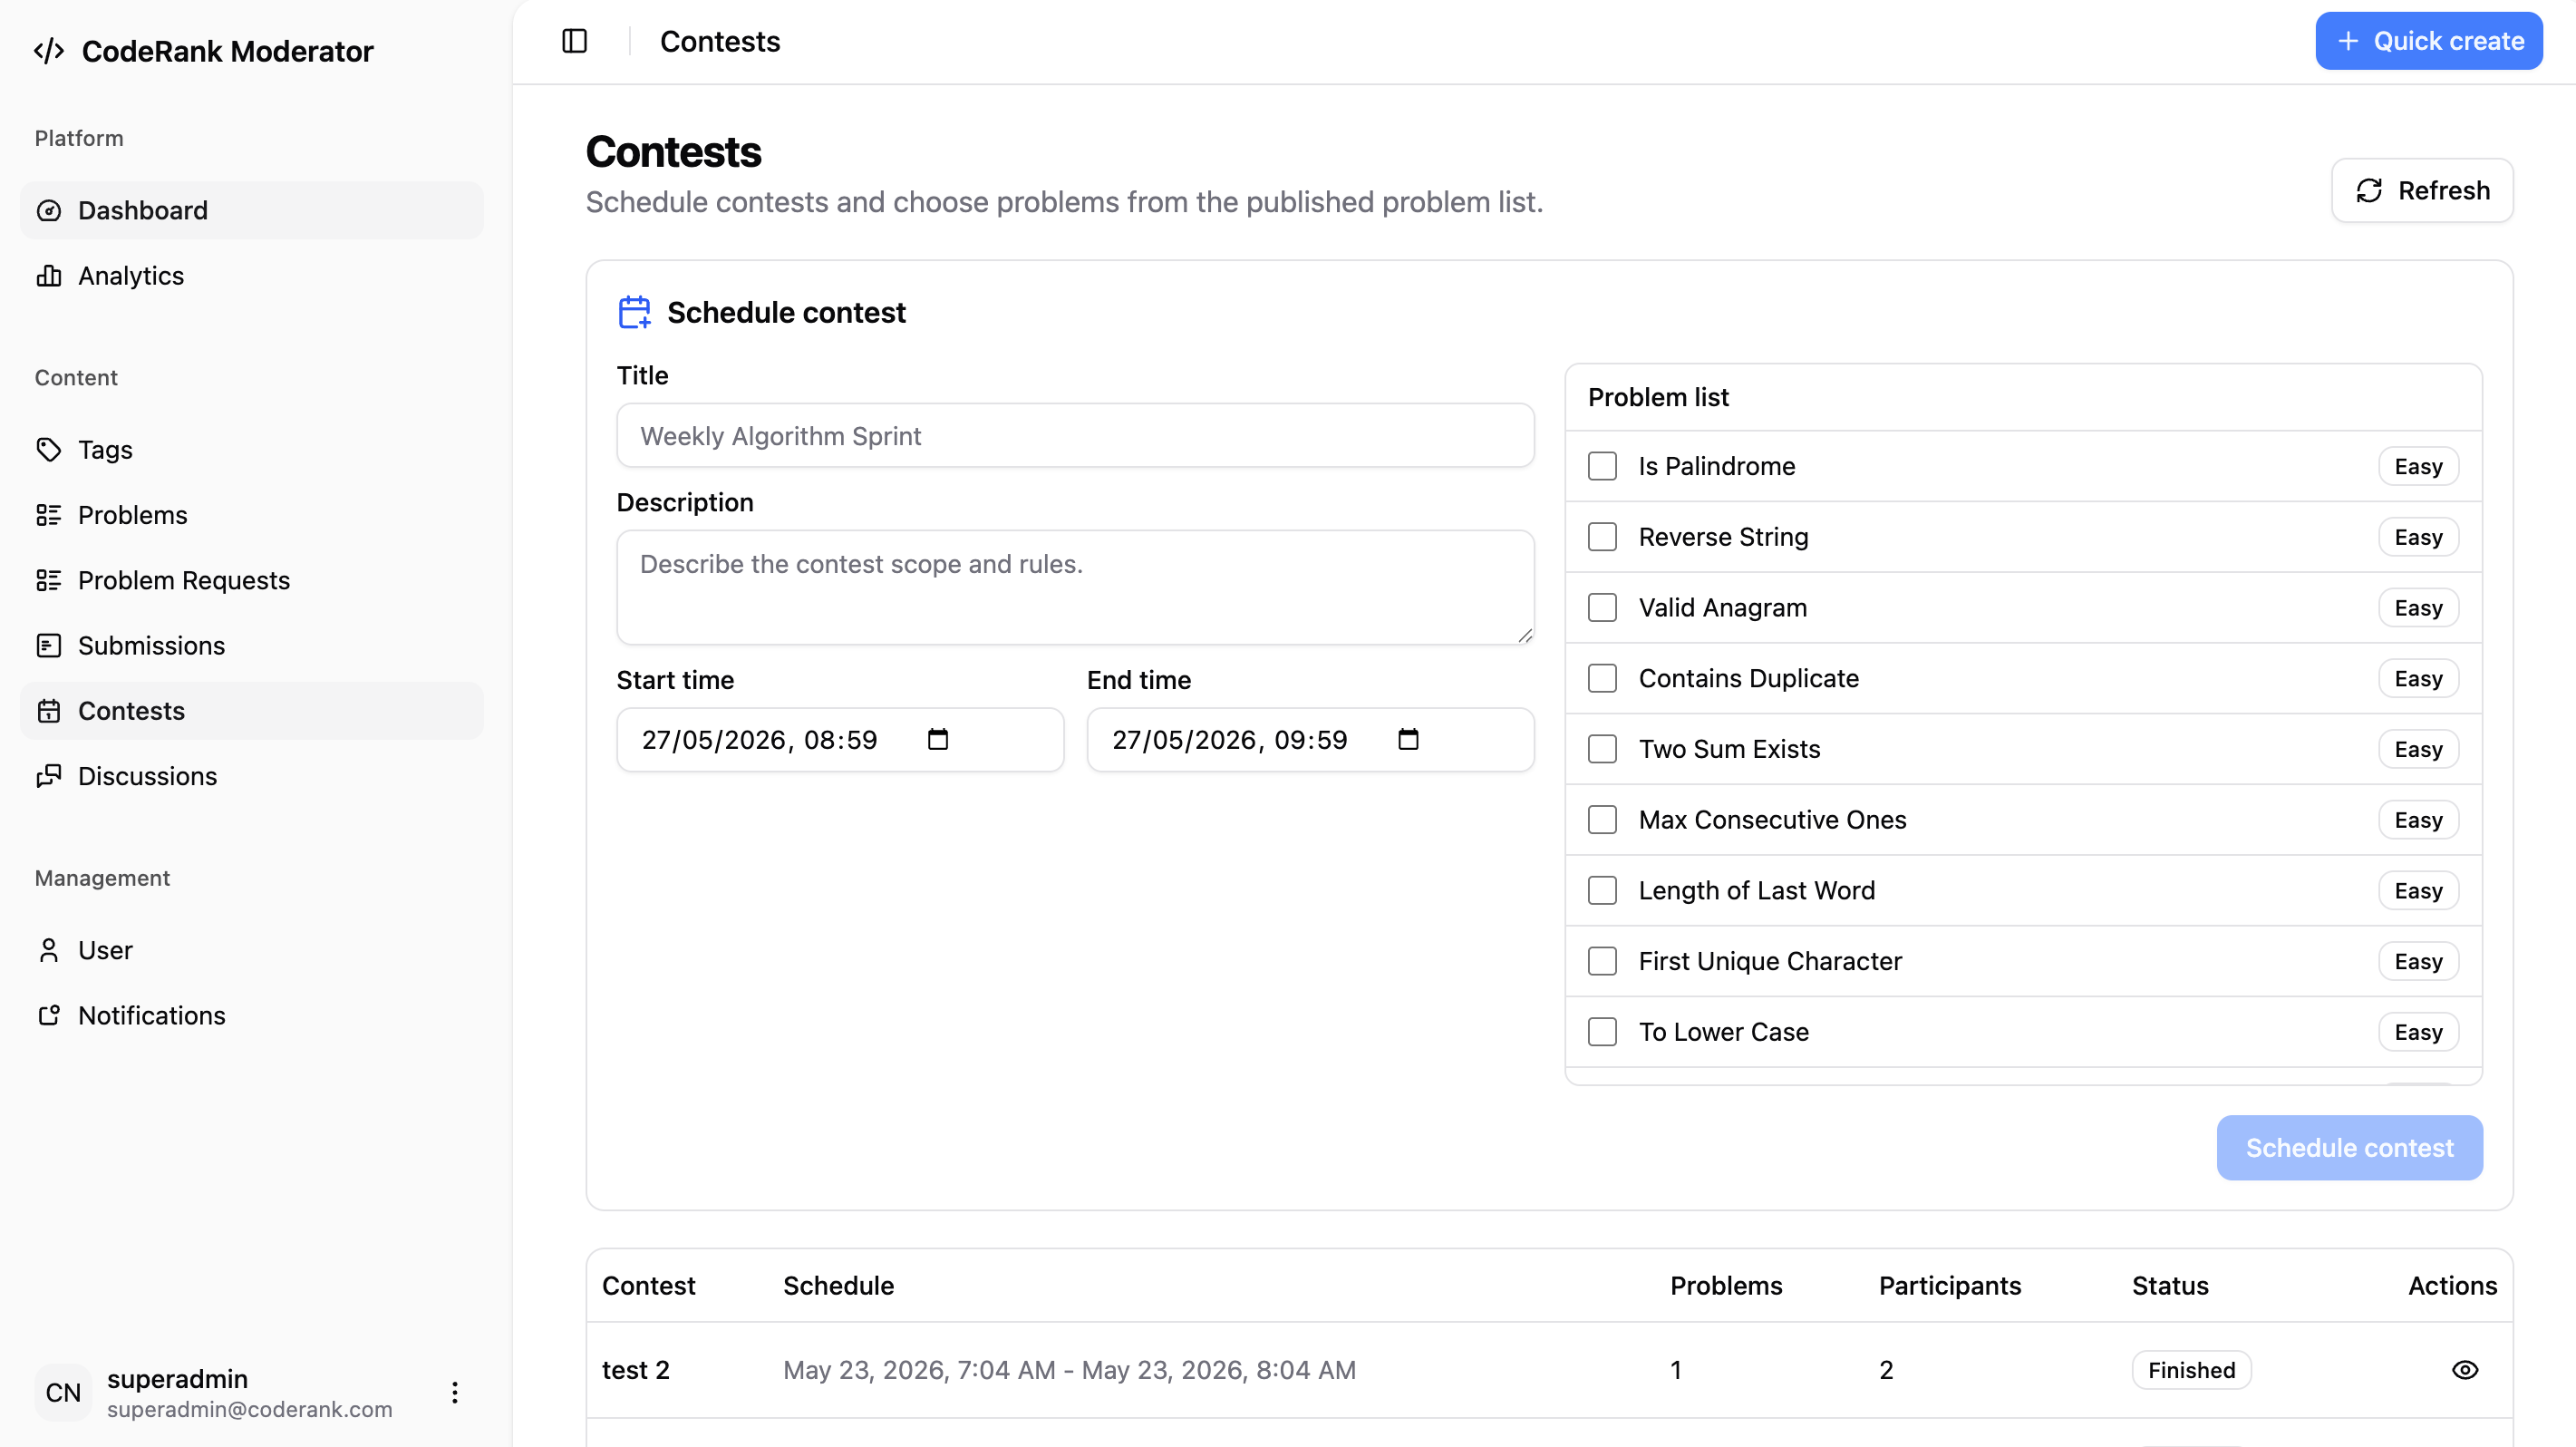
\includegraphics[width=1\textwidth]{Contents/Chapter 4/Mockup Design/Admin/contest_management.png}
    \vspace{0.6cm}
    \caption{Contest Management}
\end{figure}

The User Management interface is used to administer user accounts across the platform. It allows Moderators/Admins to view user details, delete users when required, and toggle account status to enable or disable access according to moderation decisions.
\begin{figure}[H]
    \centering
    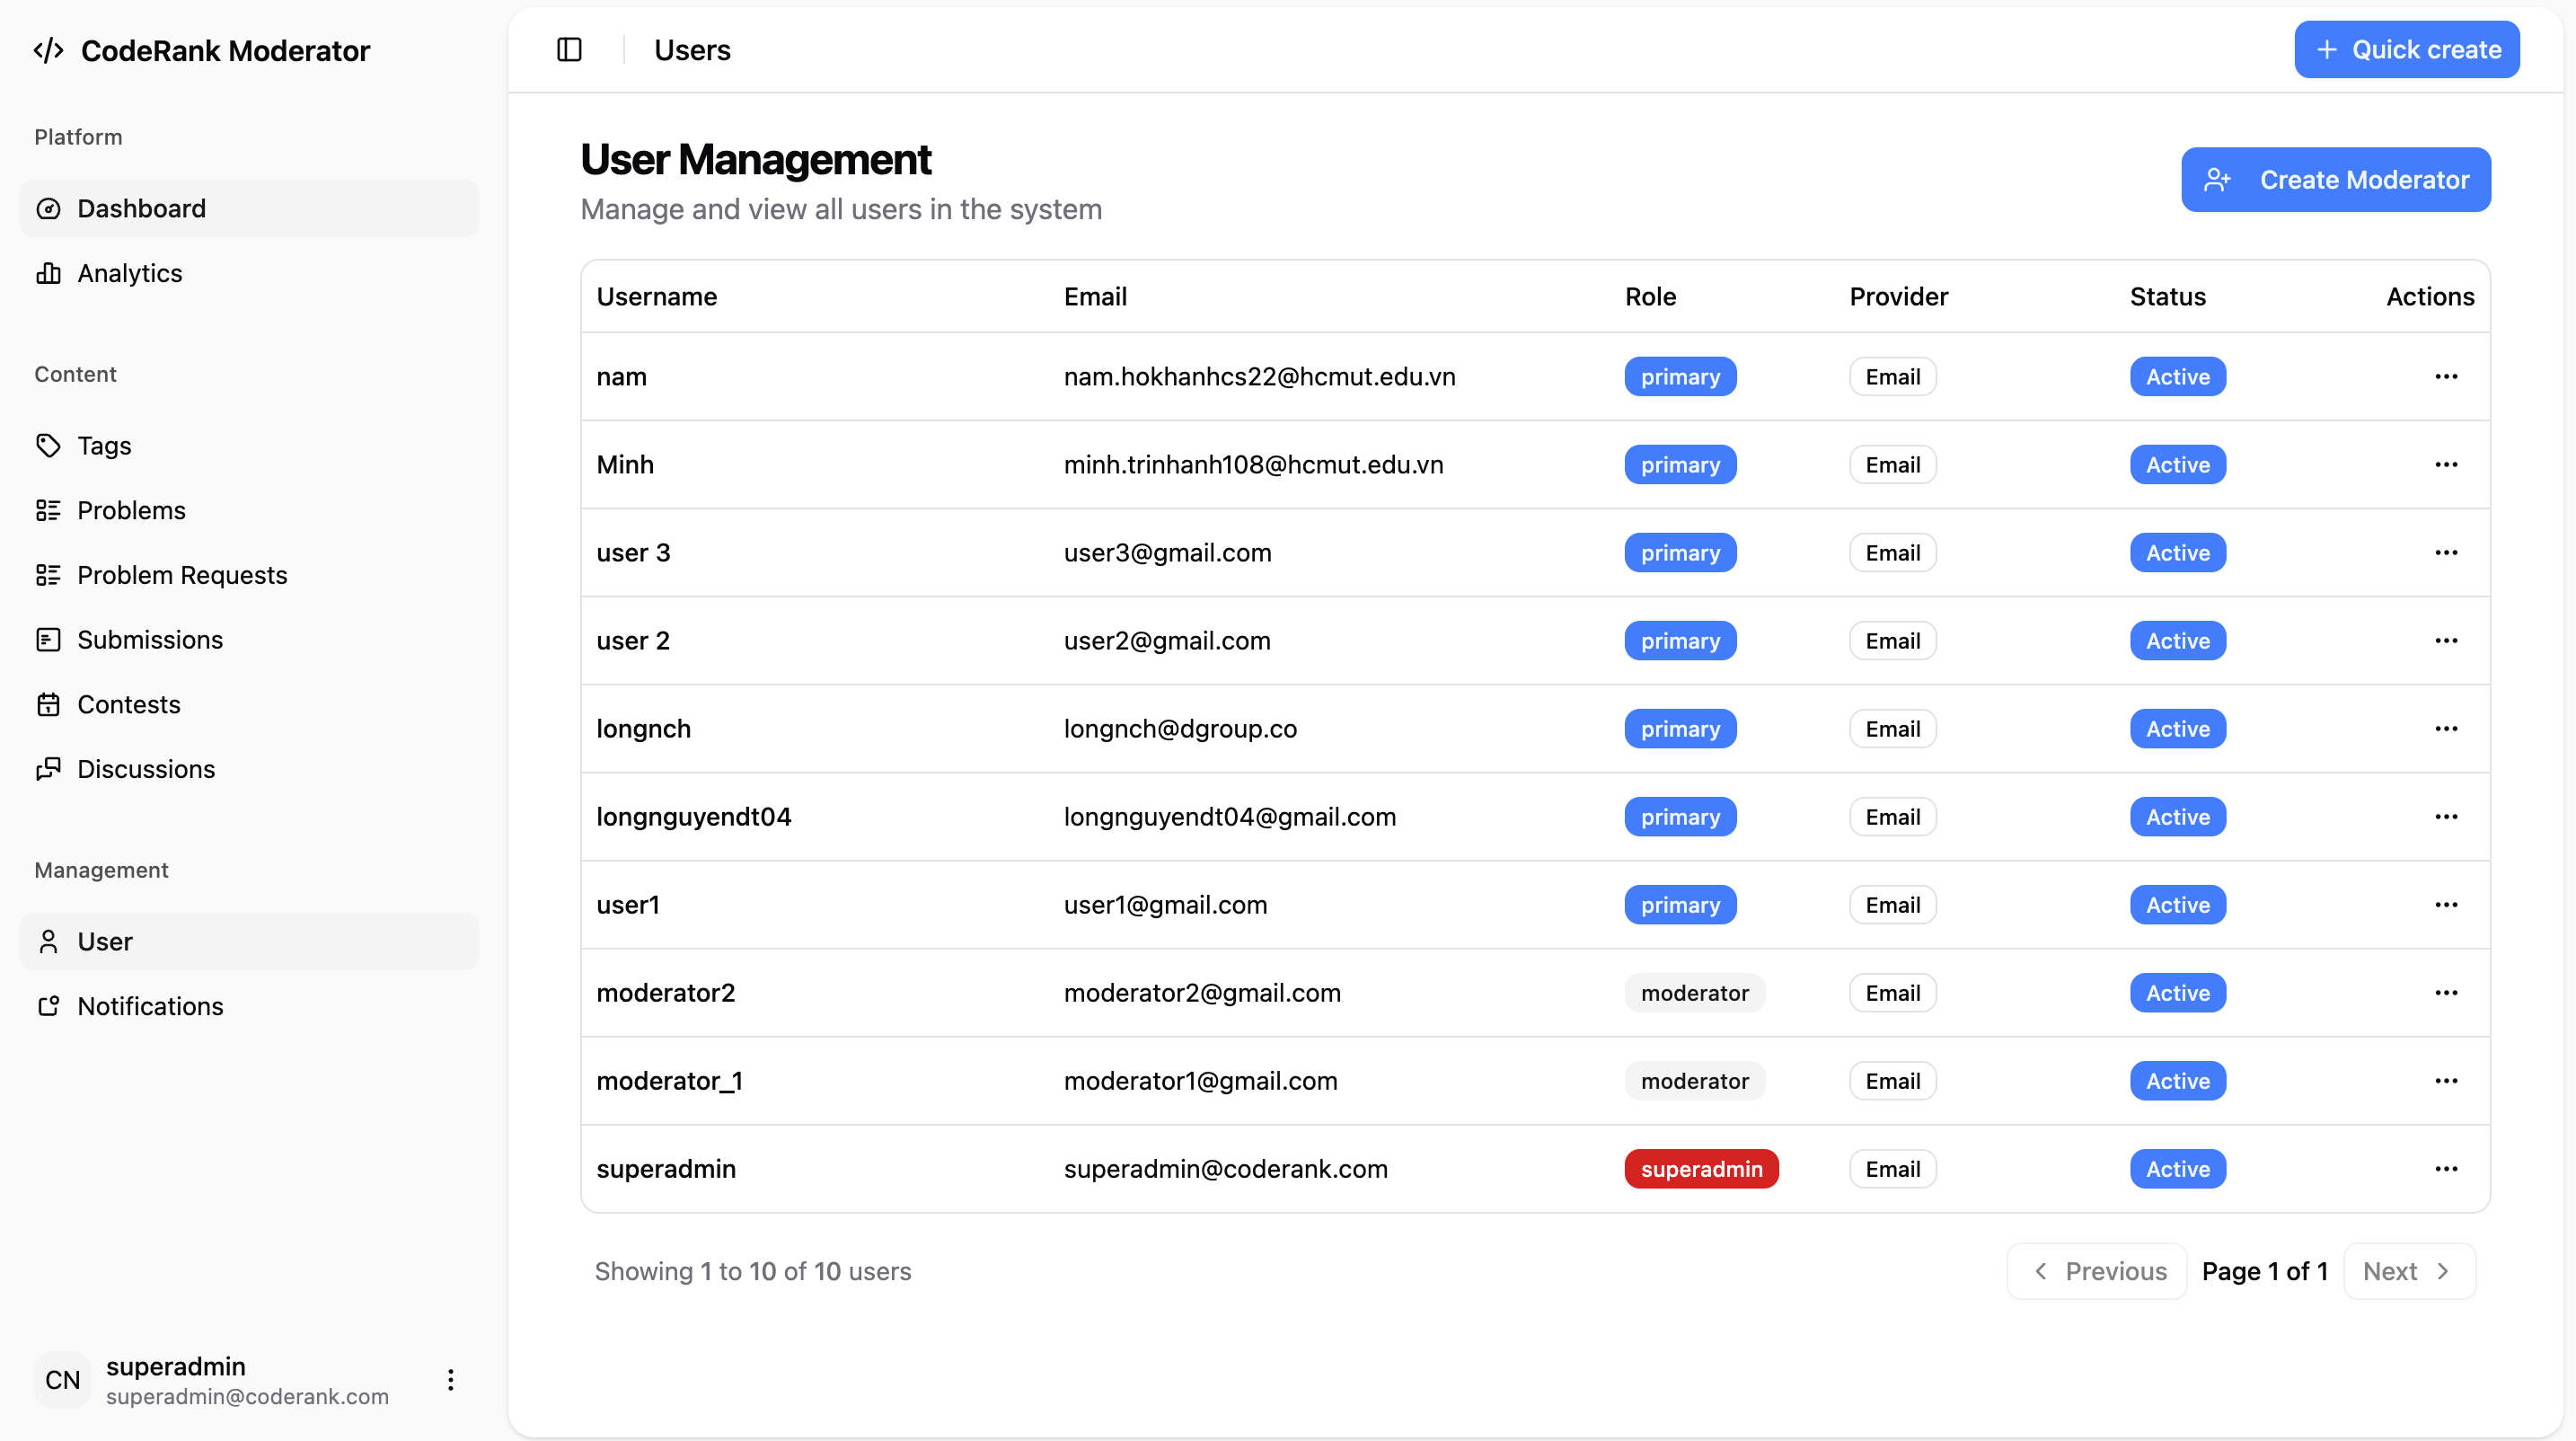
\includegraphics[width=1\textwidth]{Contents/Chapter 4/Mockup Design/Admin/user_management.png}
    \vspace{0.6cm}
    \caption{User Management}
\end{figure}

The Submission Management interface provides visibility into user submissions in the system. It helps Moderators/Admins review submission records, monitor judging results, and inspect submission-related information for operational or moderation purposes.
\begin{figure}[H]
    \centering
    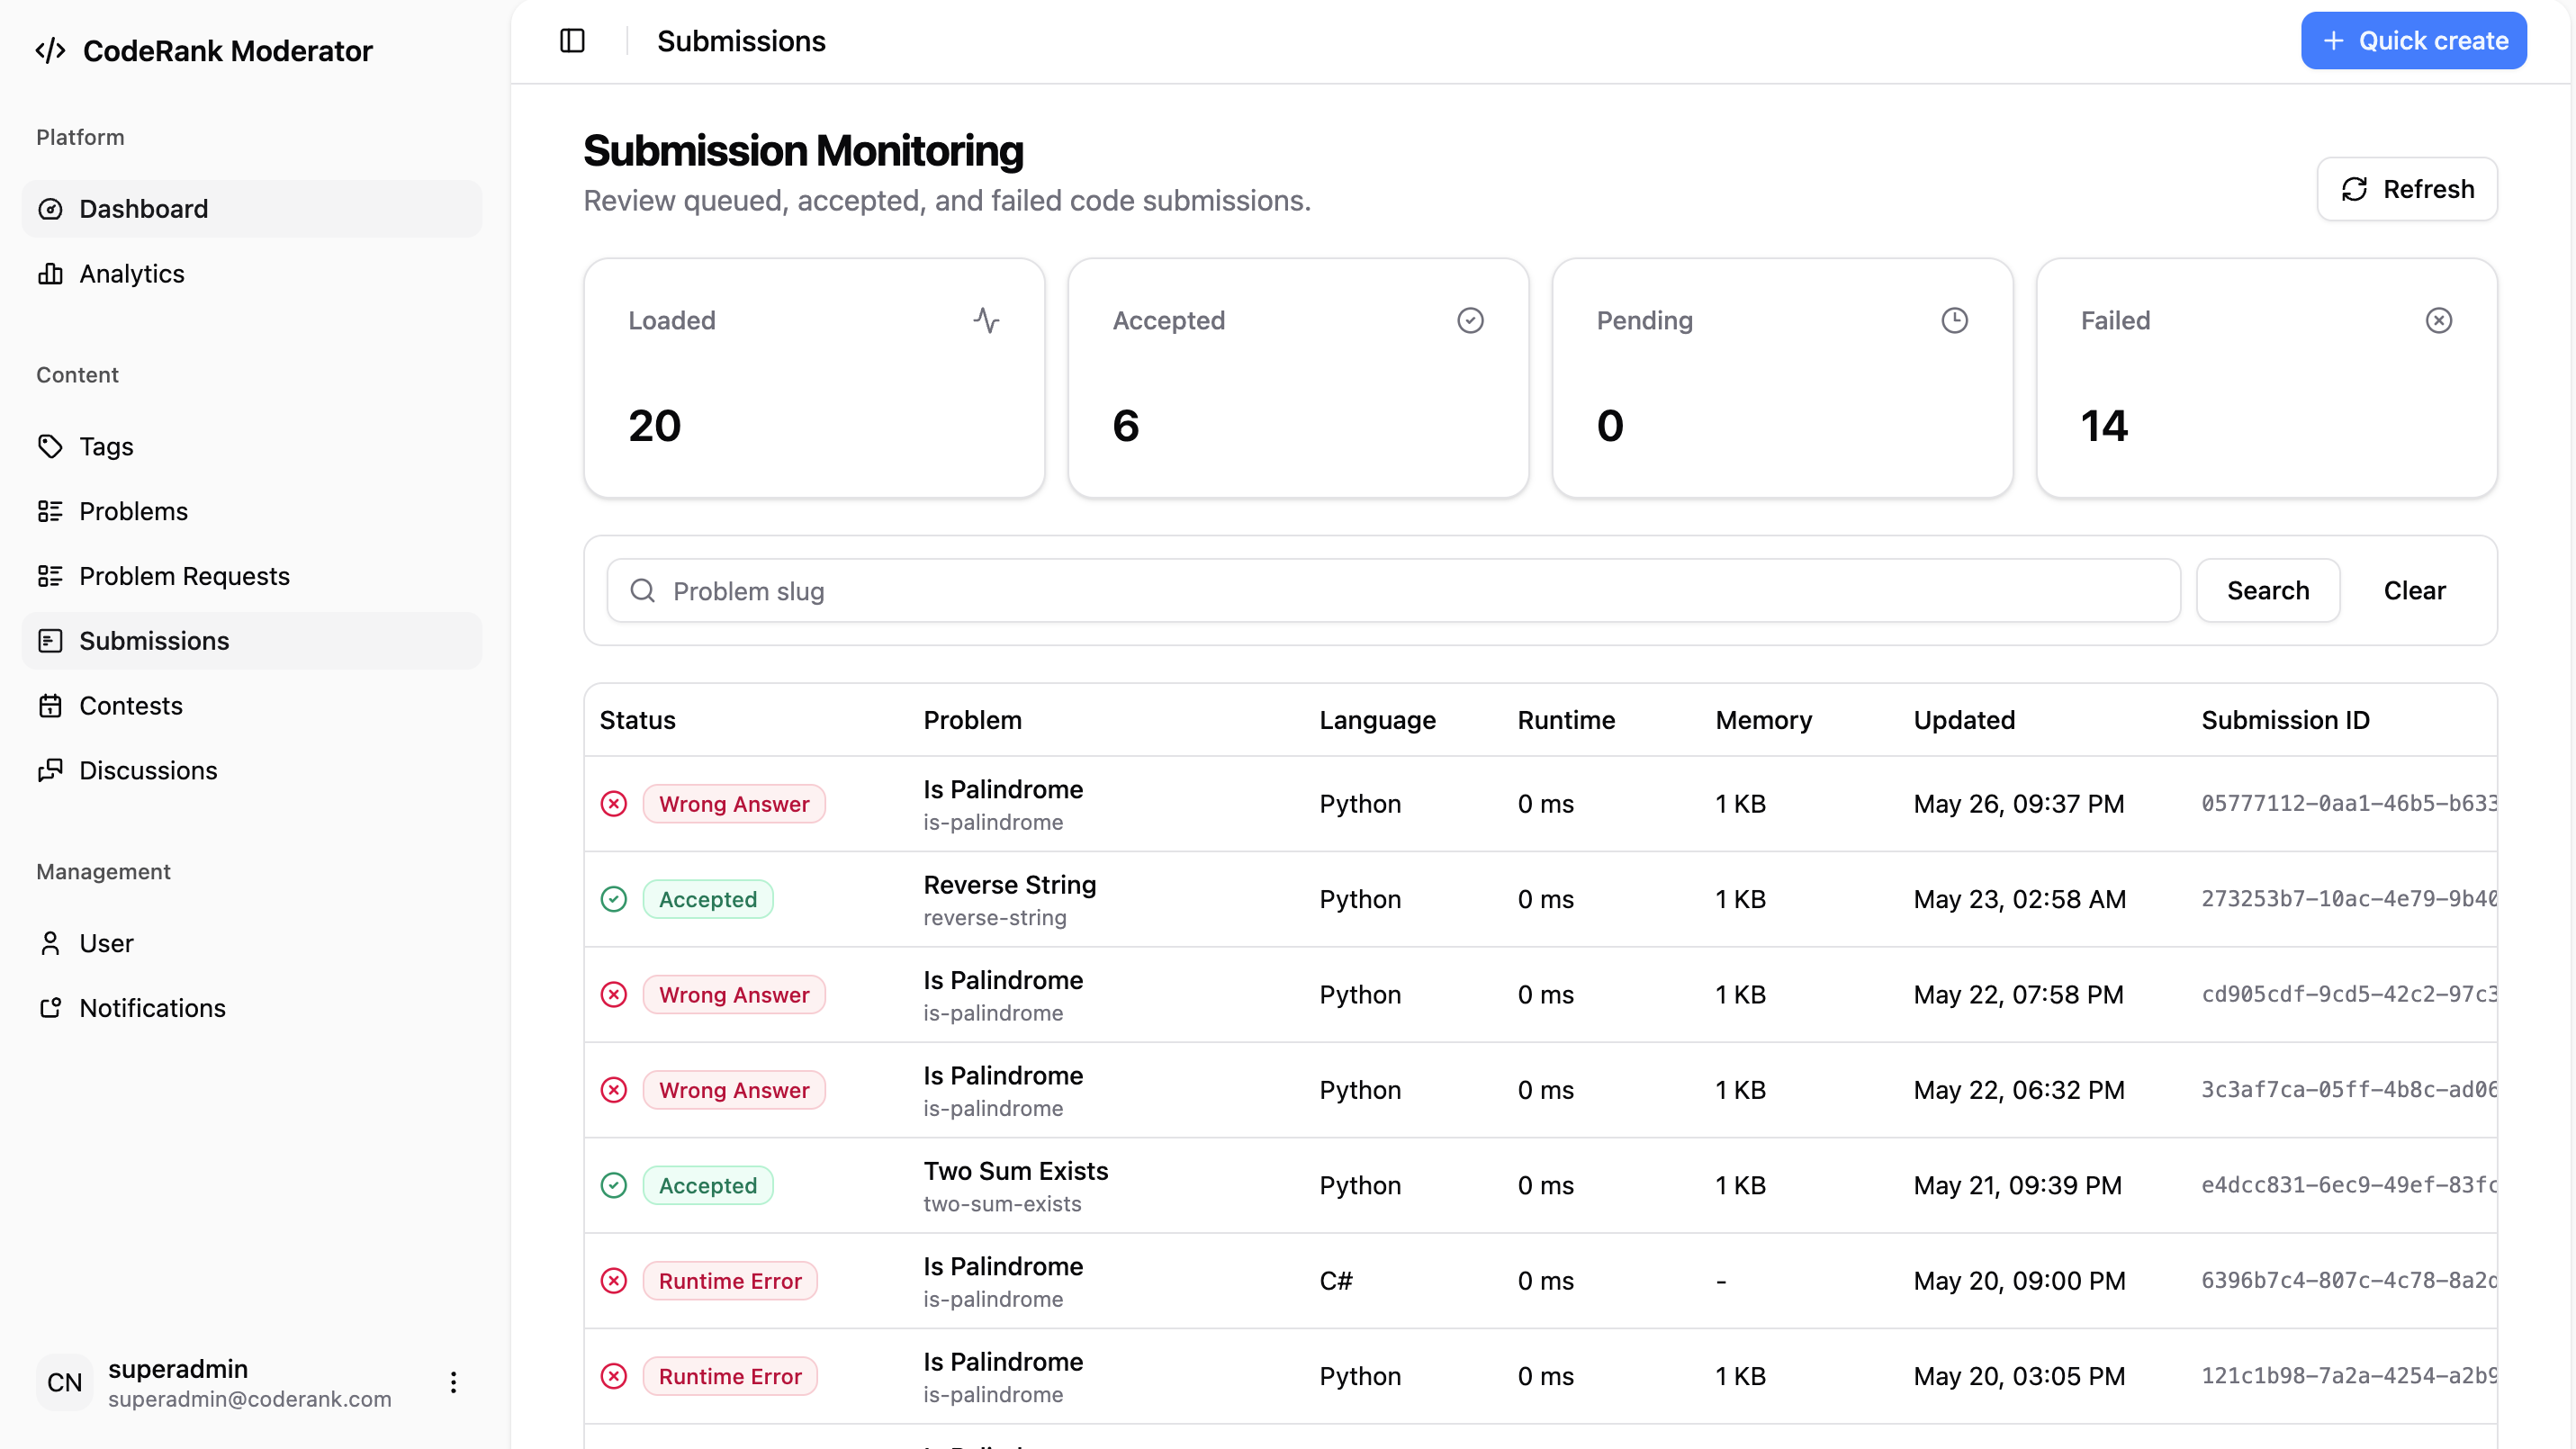
\includegraphics[width=1\textwidth]{Contents/Chapter 4/Mockup Design/Admin/submission_management.png}
    \vspace{0.6cm}
    \caption{Submission Management}
\end{figure}

The Notification Management interface is used to manage global notifications displayed on user-facing pages. Moderators/Admins can create new notifications, view existing notification details, delete outdated notifications, and control whether a notification is visible to users.
\begin{figure}[H]
    \centering
    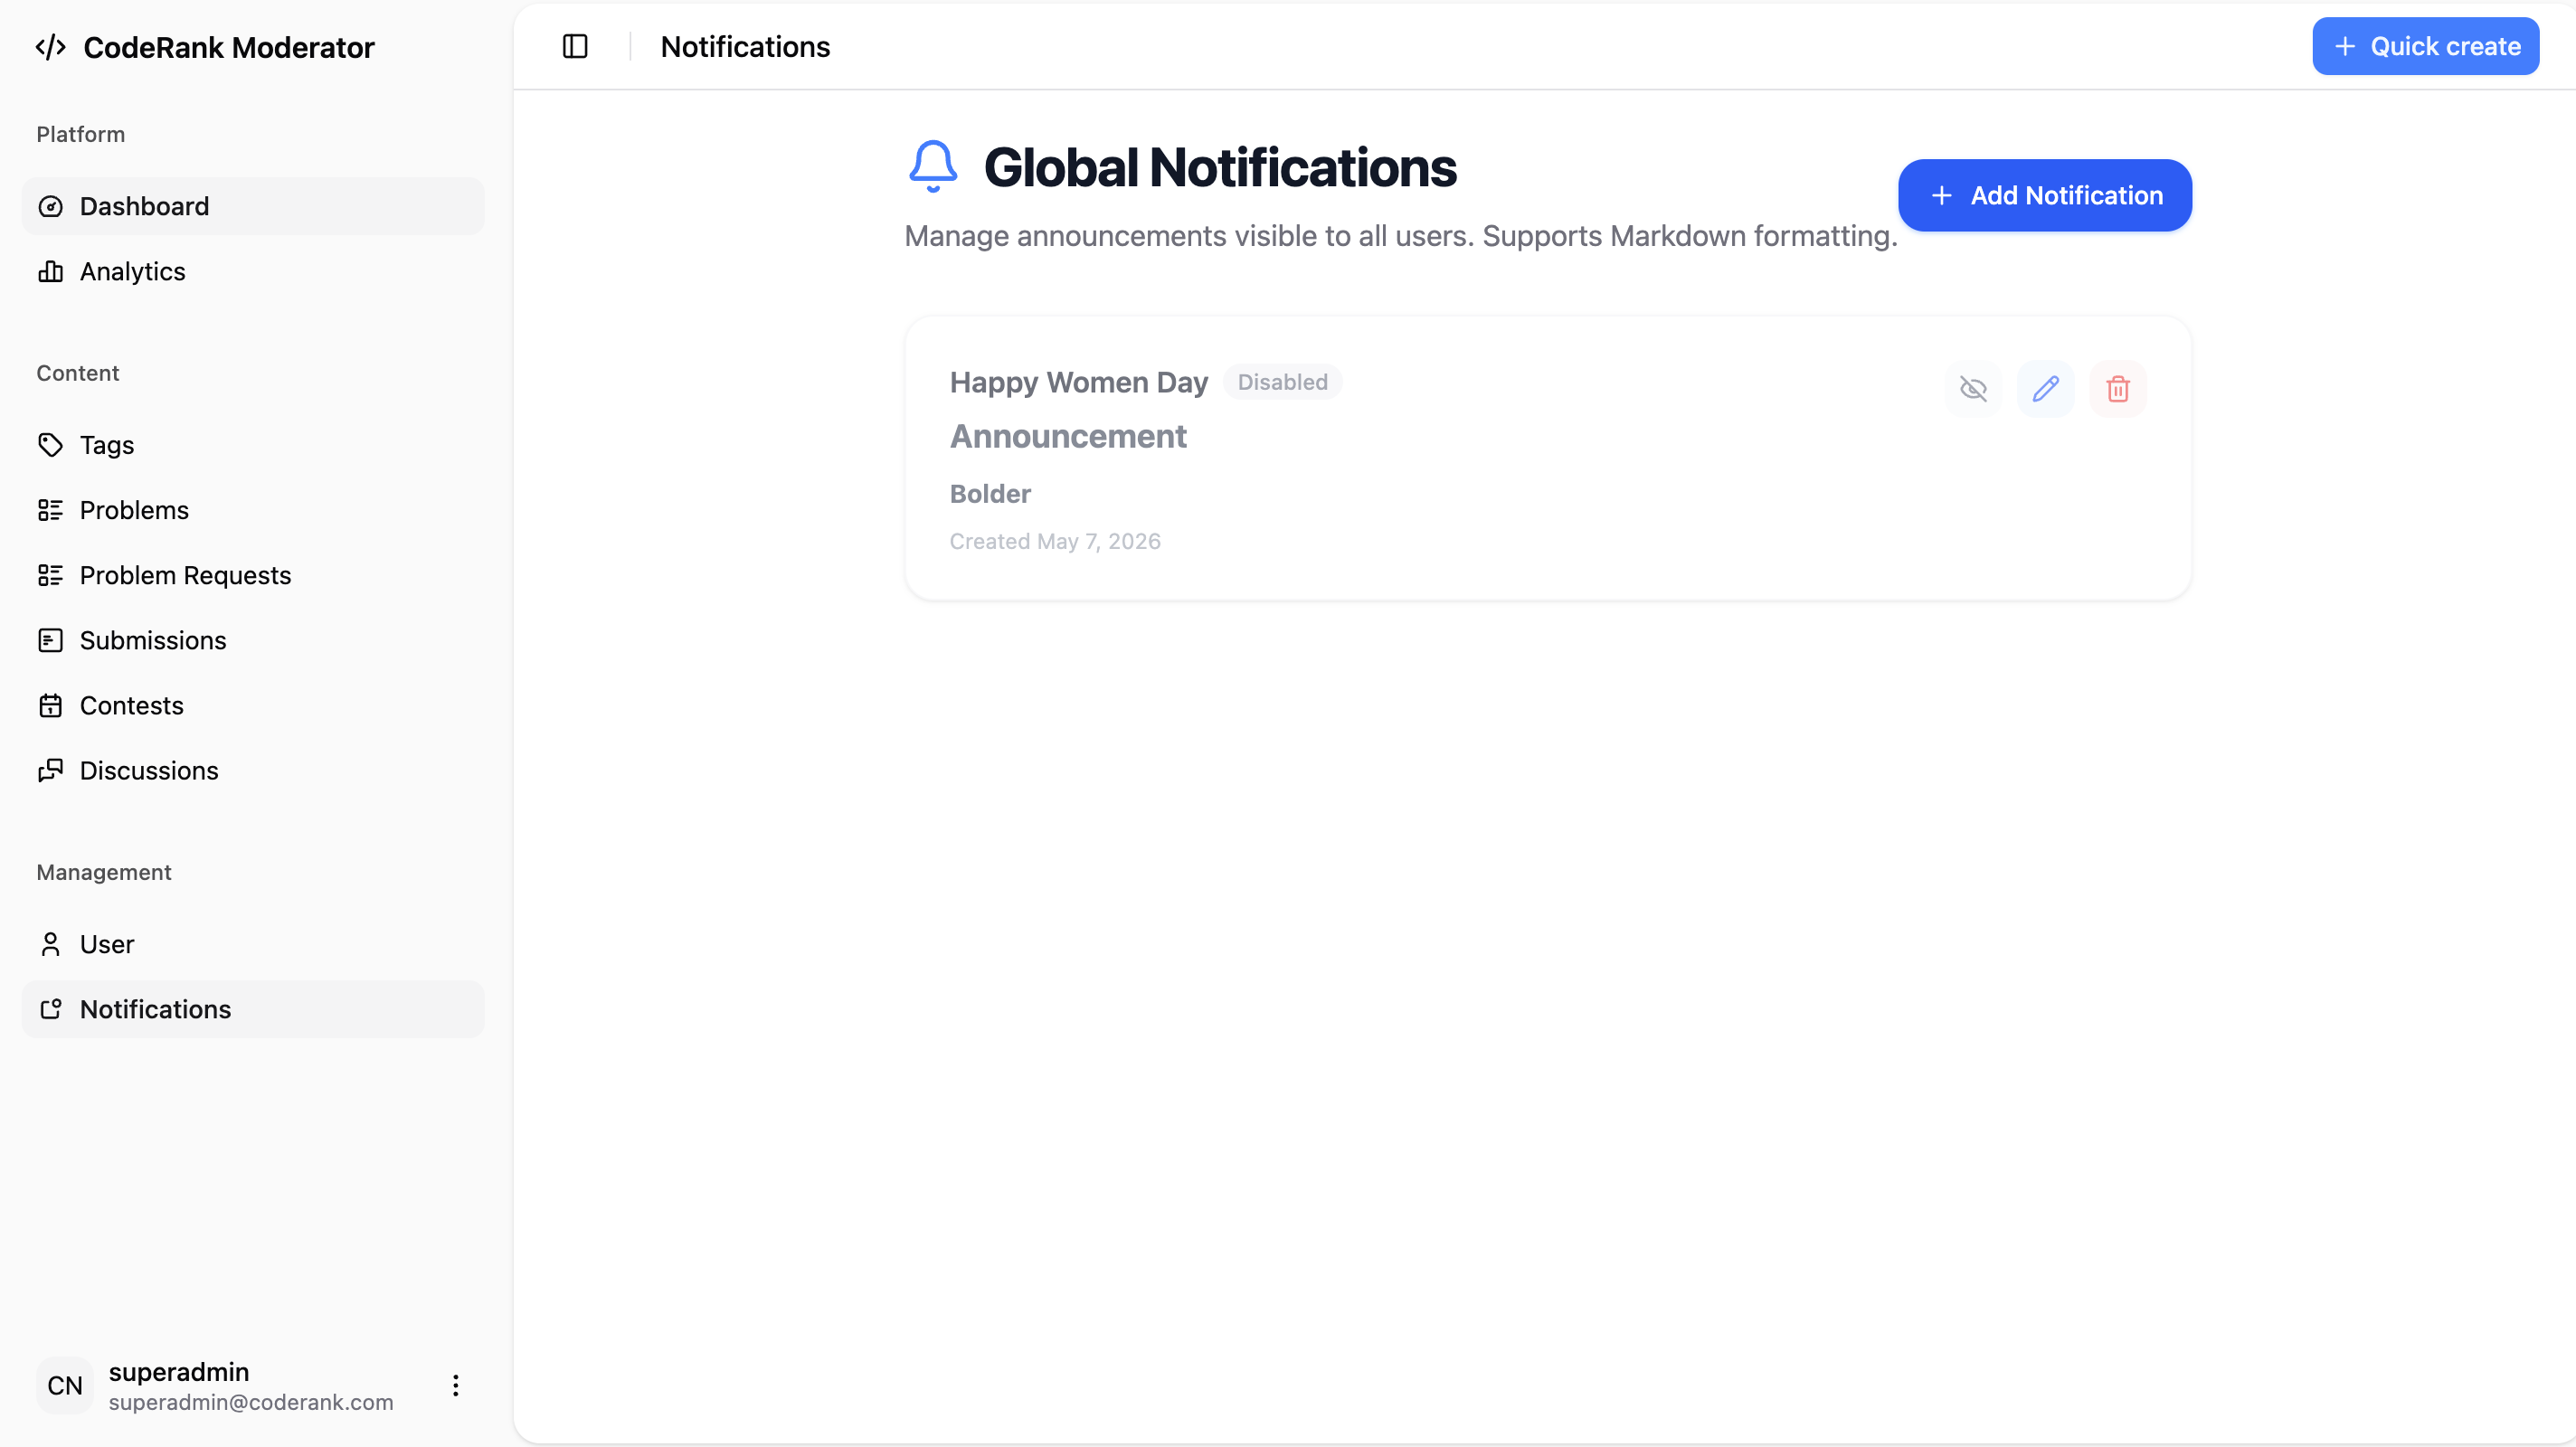
\includegraphics[width=1\textwidth]{Contents/Chapter 4/Mockup Design/Admin/notification_management.png}
    \vspace{0.6cm}
    \caption{Notification Management}
\end{figure}

Moderators/Admins can manage problem create requests submitted by another Moderator by navigating to the Problems sidebar, where a list of all problem requests is displayed along with their Difficulty level, color-coded for quick reference (Easy, Medium, Hard). In addition, this list is paginated, showing 10 items per page to ensure clear and efficient navigation.
\begin{figure}[H]
    \centering
    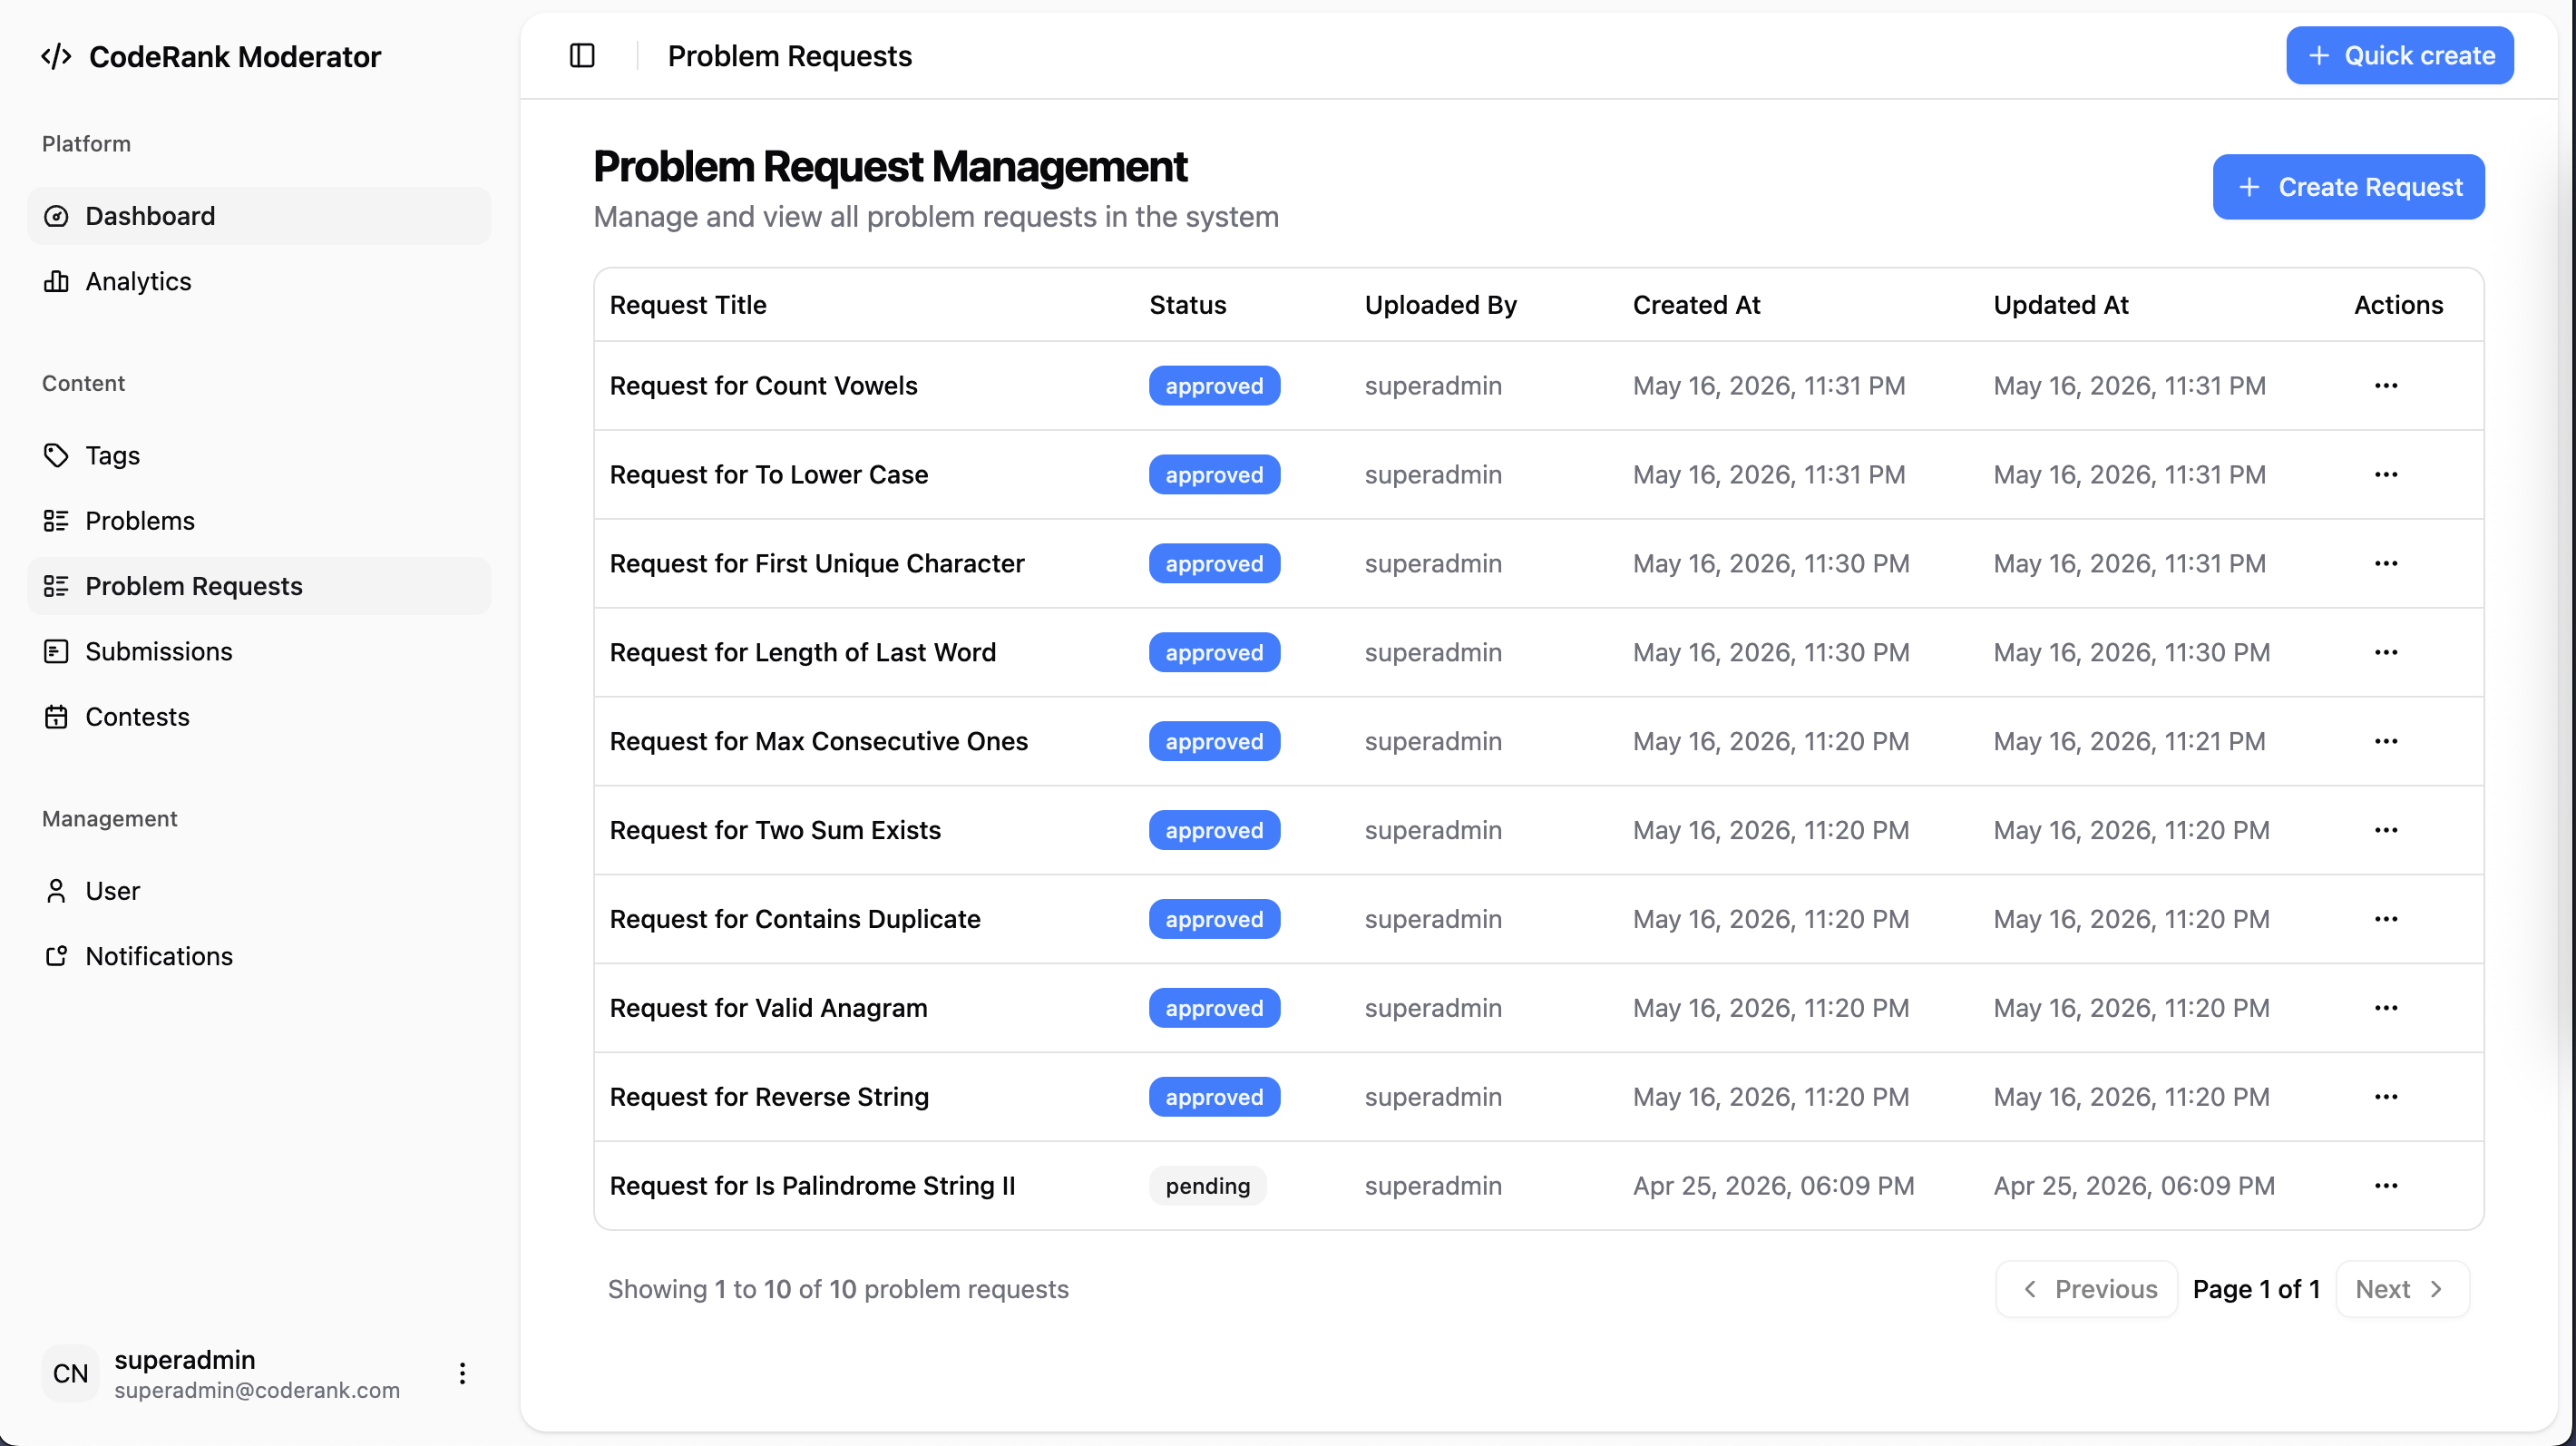
\includegraphics[width=1\textwidth]{Contents/Chapter 4/Mockup Design/Admin/Problem_request_list.png}
    \vspace{0.6cm}
    \caption{Problem Request List}
\end{figure}


A “Create Problem” button is positioned at the top-right corner of the interface, allowing users to quickly submit a new problem request. When this button is clicked, a creation modal appears centered on the screen, enabling Moderators/Admins to input all necessary details, in which user is required to fill in fields such as Problem Name, Difficulty level, Topic, and any other relevant information needed to define the problem.
\begin{figure}[H]
    \centering
    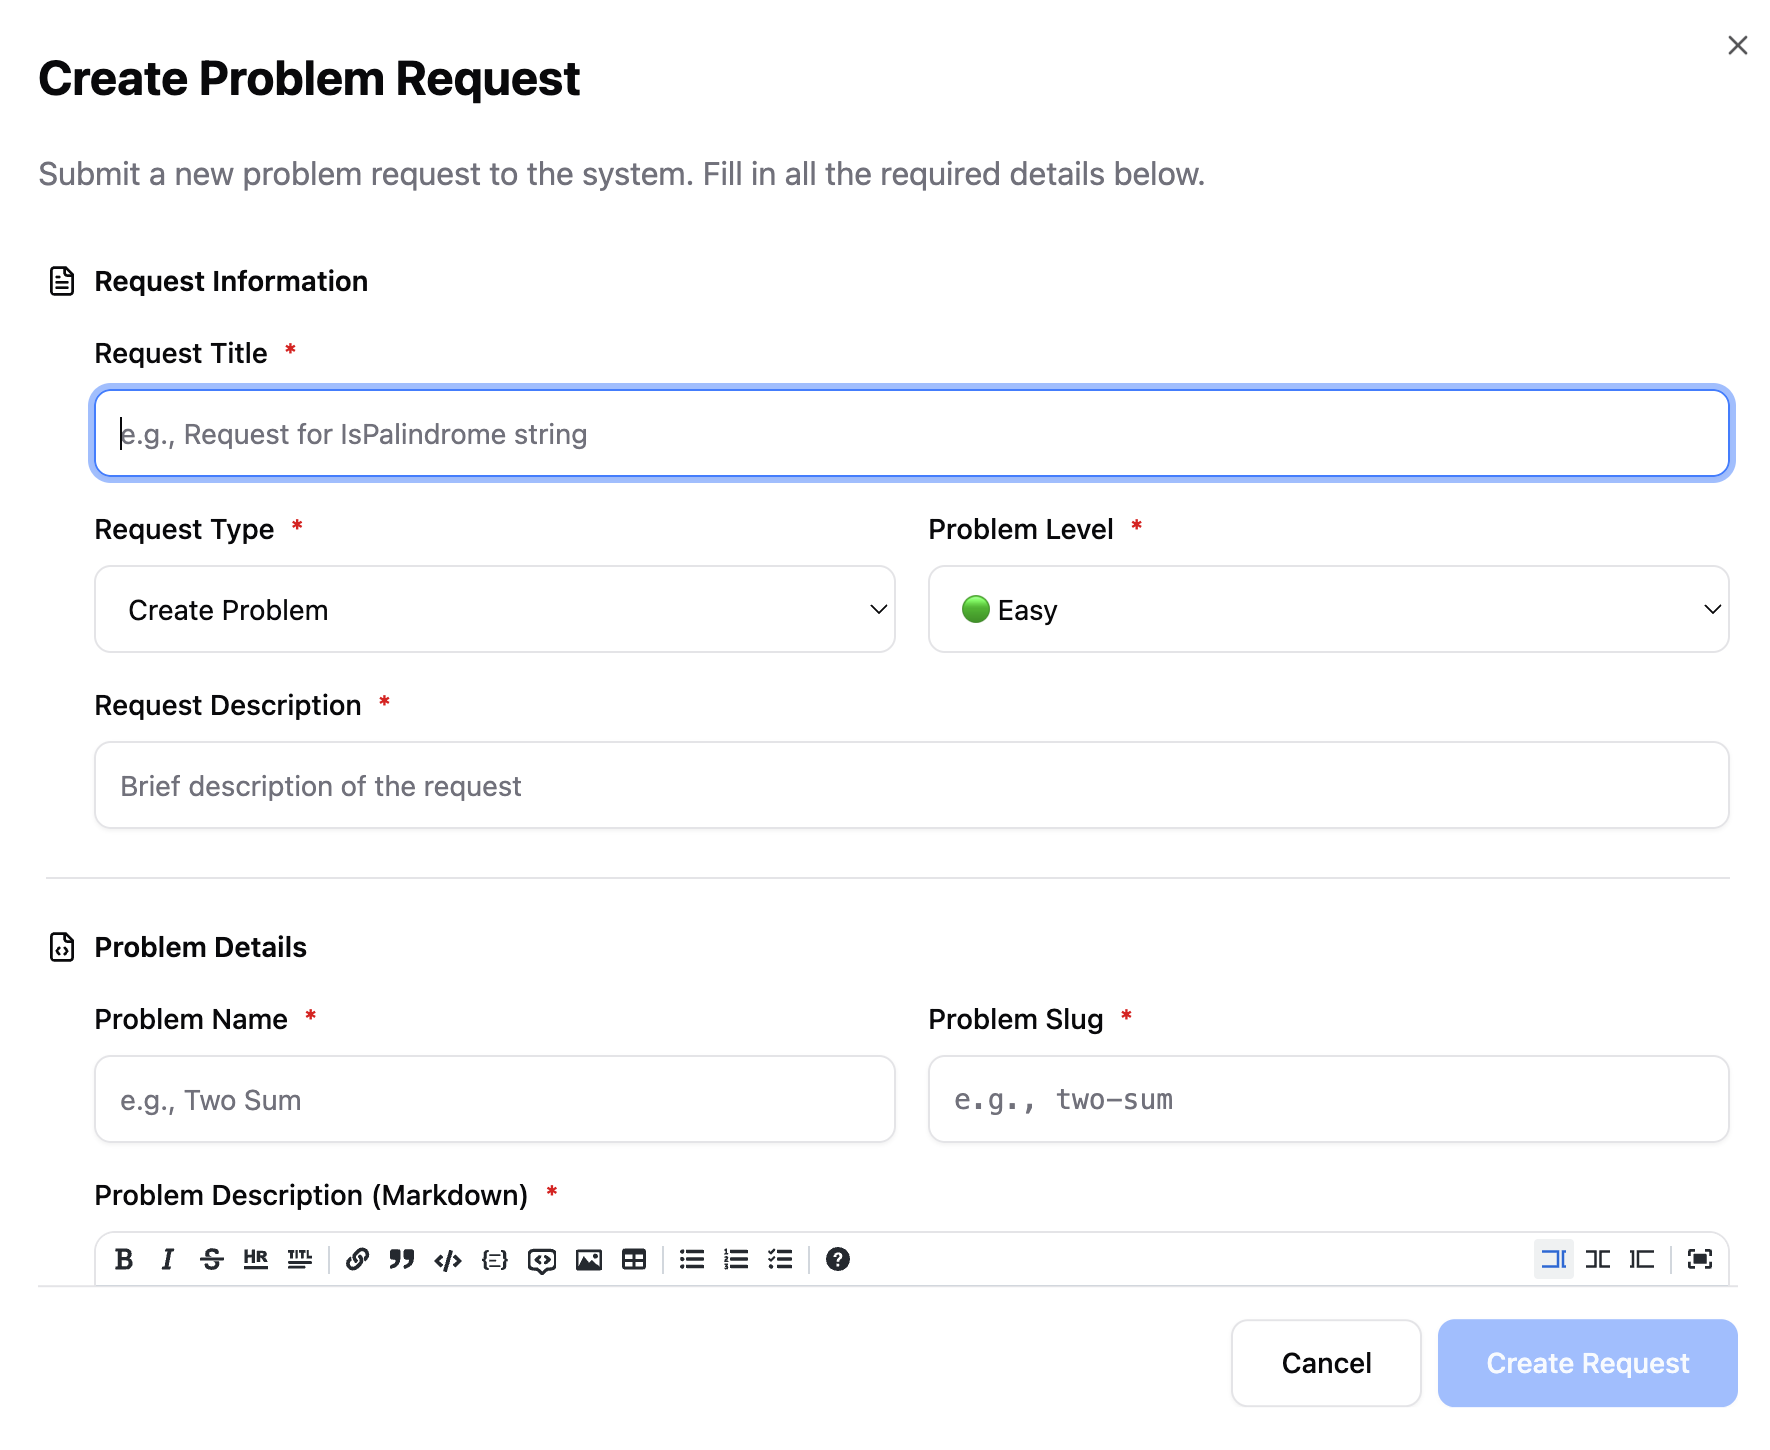
\includegraphics[width=1\textwidth]{Contents/Chapter 4/Mockup Design/Admin/Problem_request_modal.png}
    \vspace{0.6cm}
    \caption{Problem Request Create Modal}
\end{figure}

Moderators can also monitor submissions in real-time by navigating to the Submissions sidebar. This page displays a list of all submissions made by users, along with relevant details such as submission ID, user name, problem name, status (e.g., Accepted, Wrong Answer, Time Limit Exceeded), and submission time. Moderators can filter and sort the submissions based on various criteria to quickly identify any issues or patterns in user submissions.
\begin{figure}[H]
    \centering
    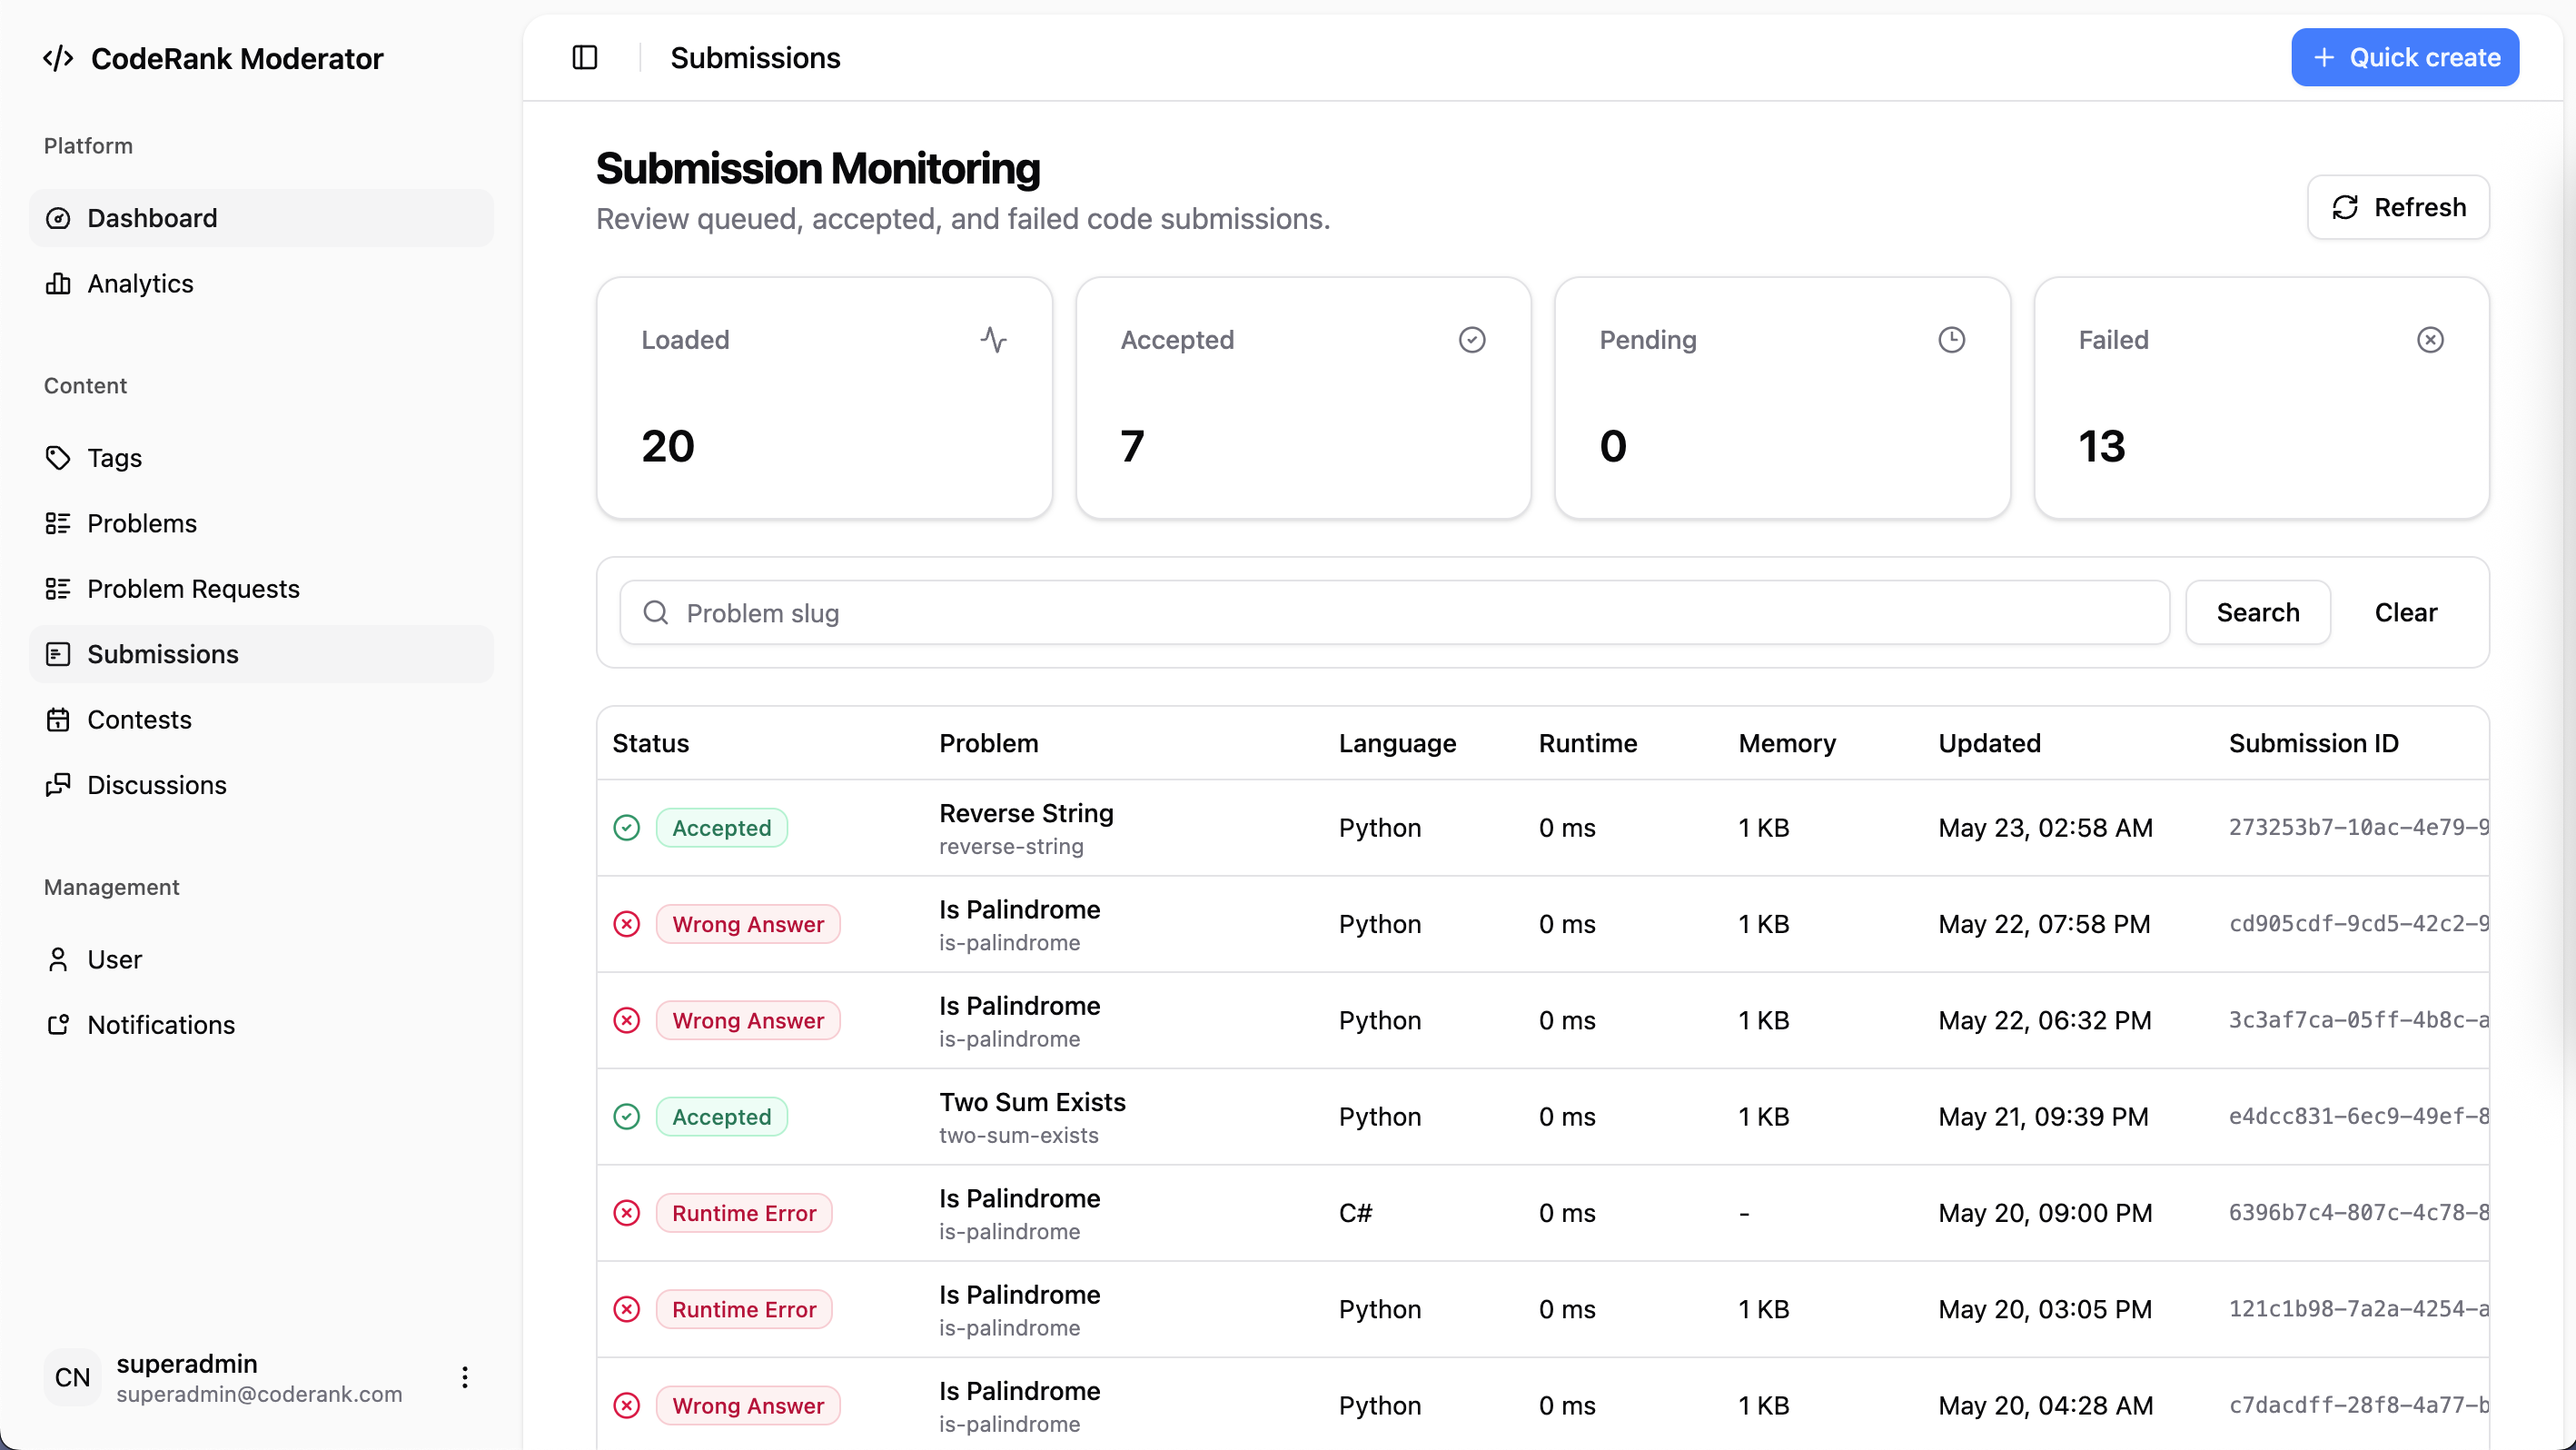
\includegraphics[width=1\textwidth]{Contents/Chapter 4/Mockup Design/Admin/submission_monitor.png}
    \vspace{0.6cm}
    \caption{Submission Monitor}
\end{figure}

Beside submissions, moderators can also monitor current discussions by navigating to the Discussions sidebar. This page displays a list of all active discussion threads, along with relevant details such as thread title, topic, number of messages, and last activity time. Moderators can filter and sort the discussions based on various criteria to quickly identify any issues or patterns in user discussions.
\begin{figure}[H]
    \centering
    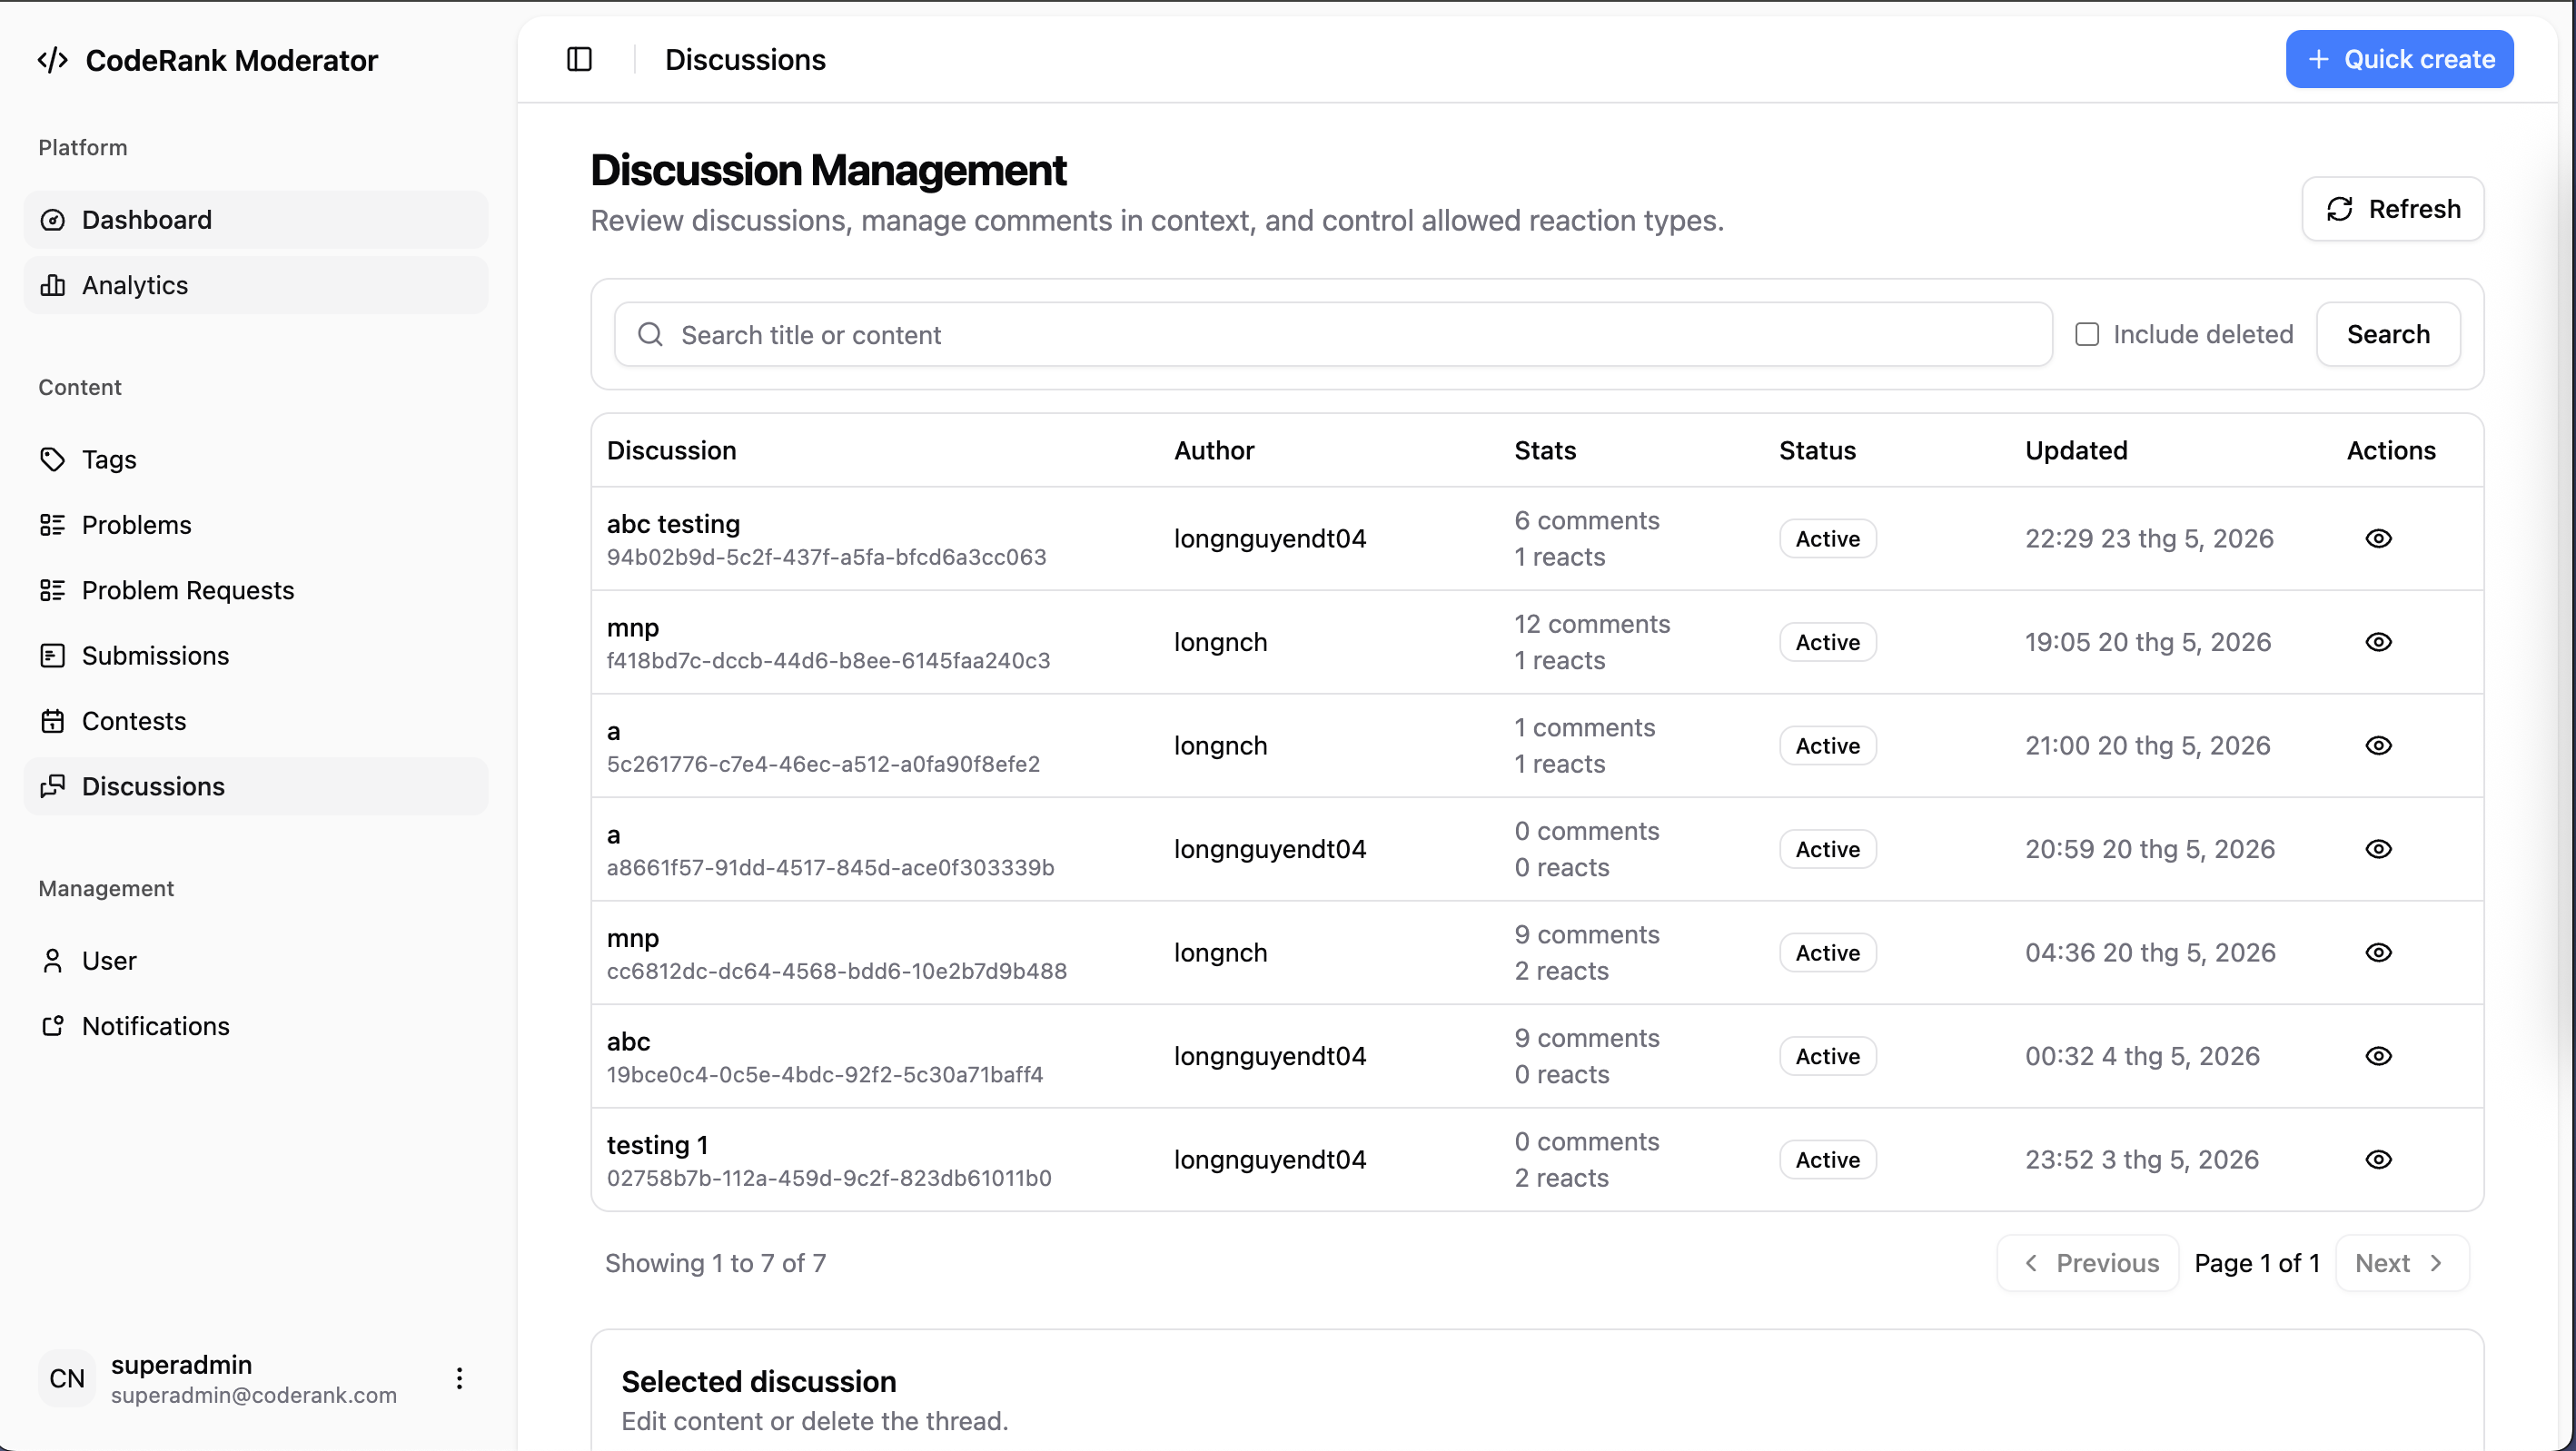
\includegraphics[width=1\textwidth]{Contents/Chapter 4/Mockup Design/Admin/discussion_monitor.png}
    \vspace{0.6cm}
    \caption{Discussion Monitor}
\end{figure}

Moderator can also managing notifications and announcements to all users by navigating to the Notifications sidebar. This page displays a list of all notifications sent to users, along with relevant details such as notification type, recipient user name, content summary, and timestamp. Moderators can filter and sort the notifications based on various criteria to quickly identify any issues or patterns in user notifications.
\begin{figure}[H]
    \centering
    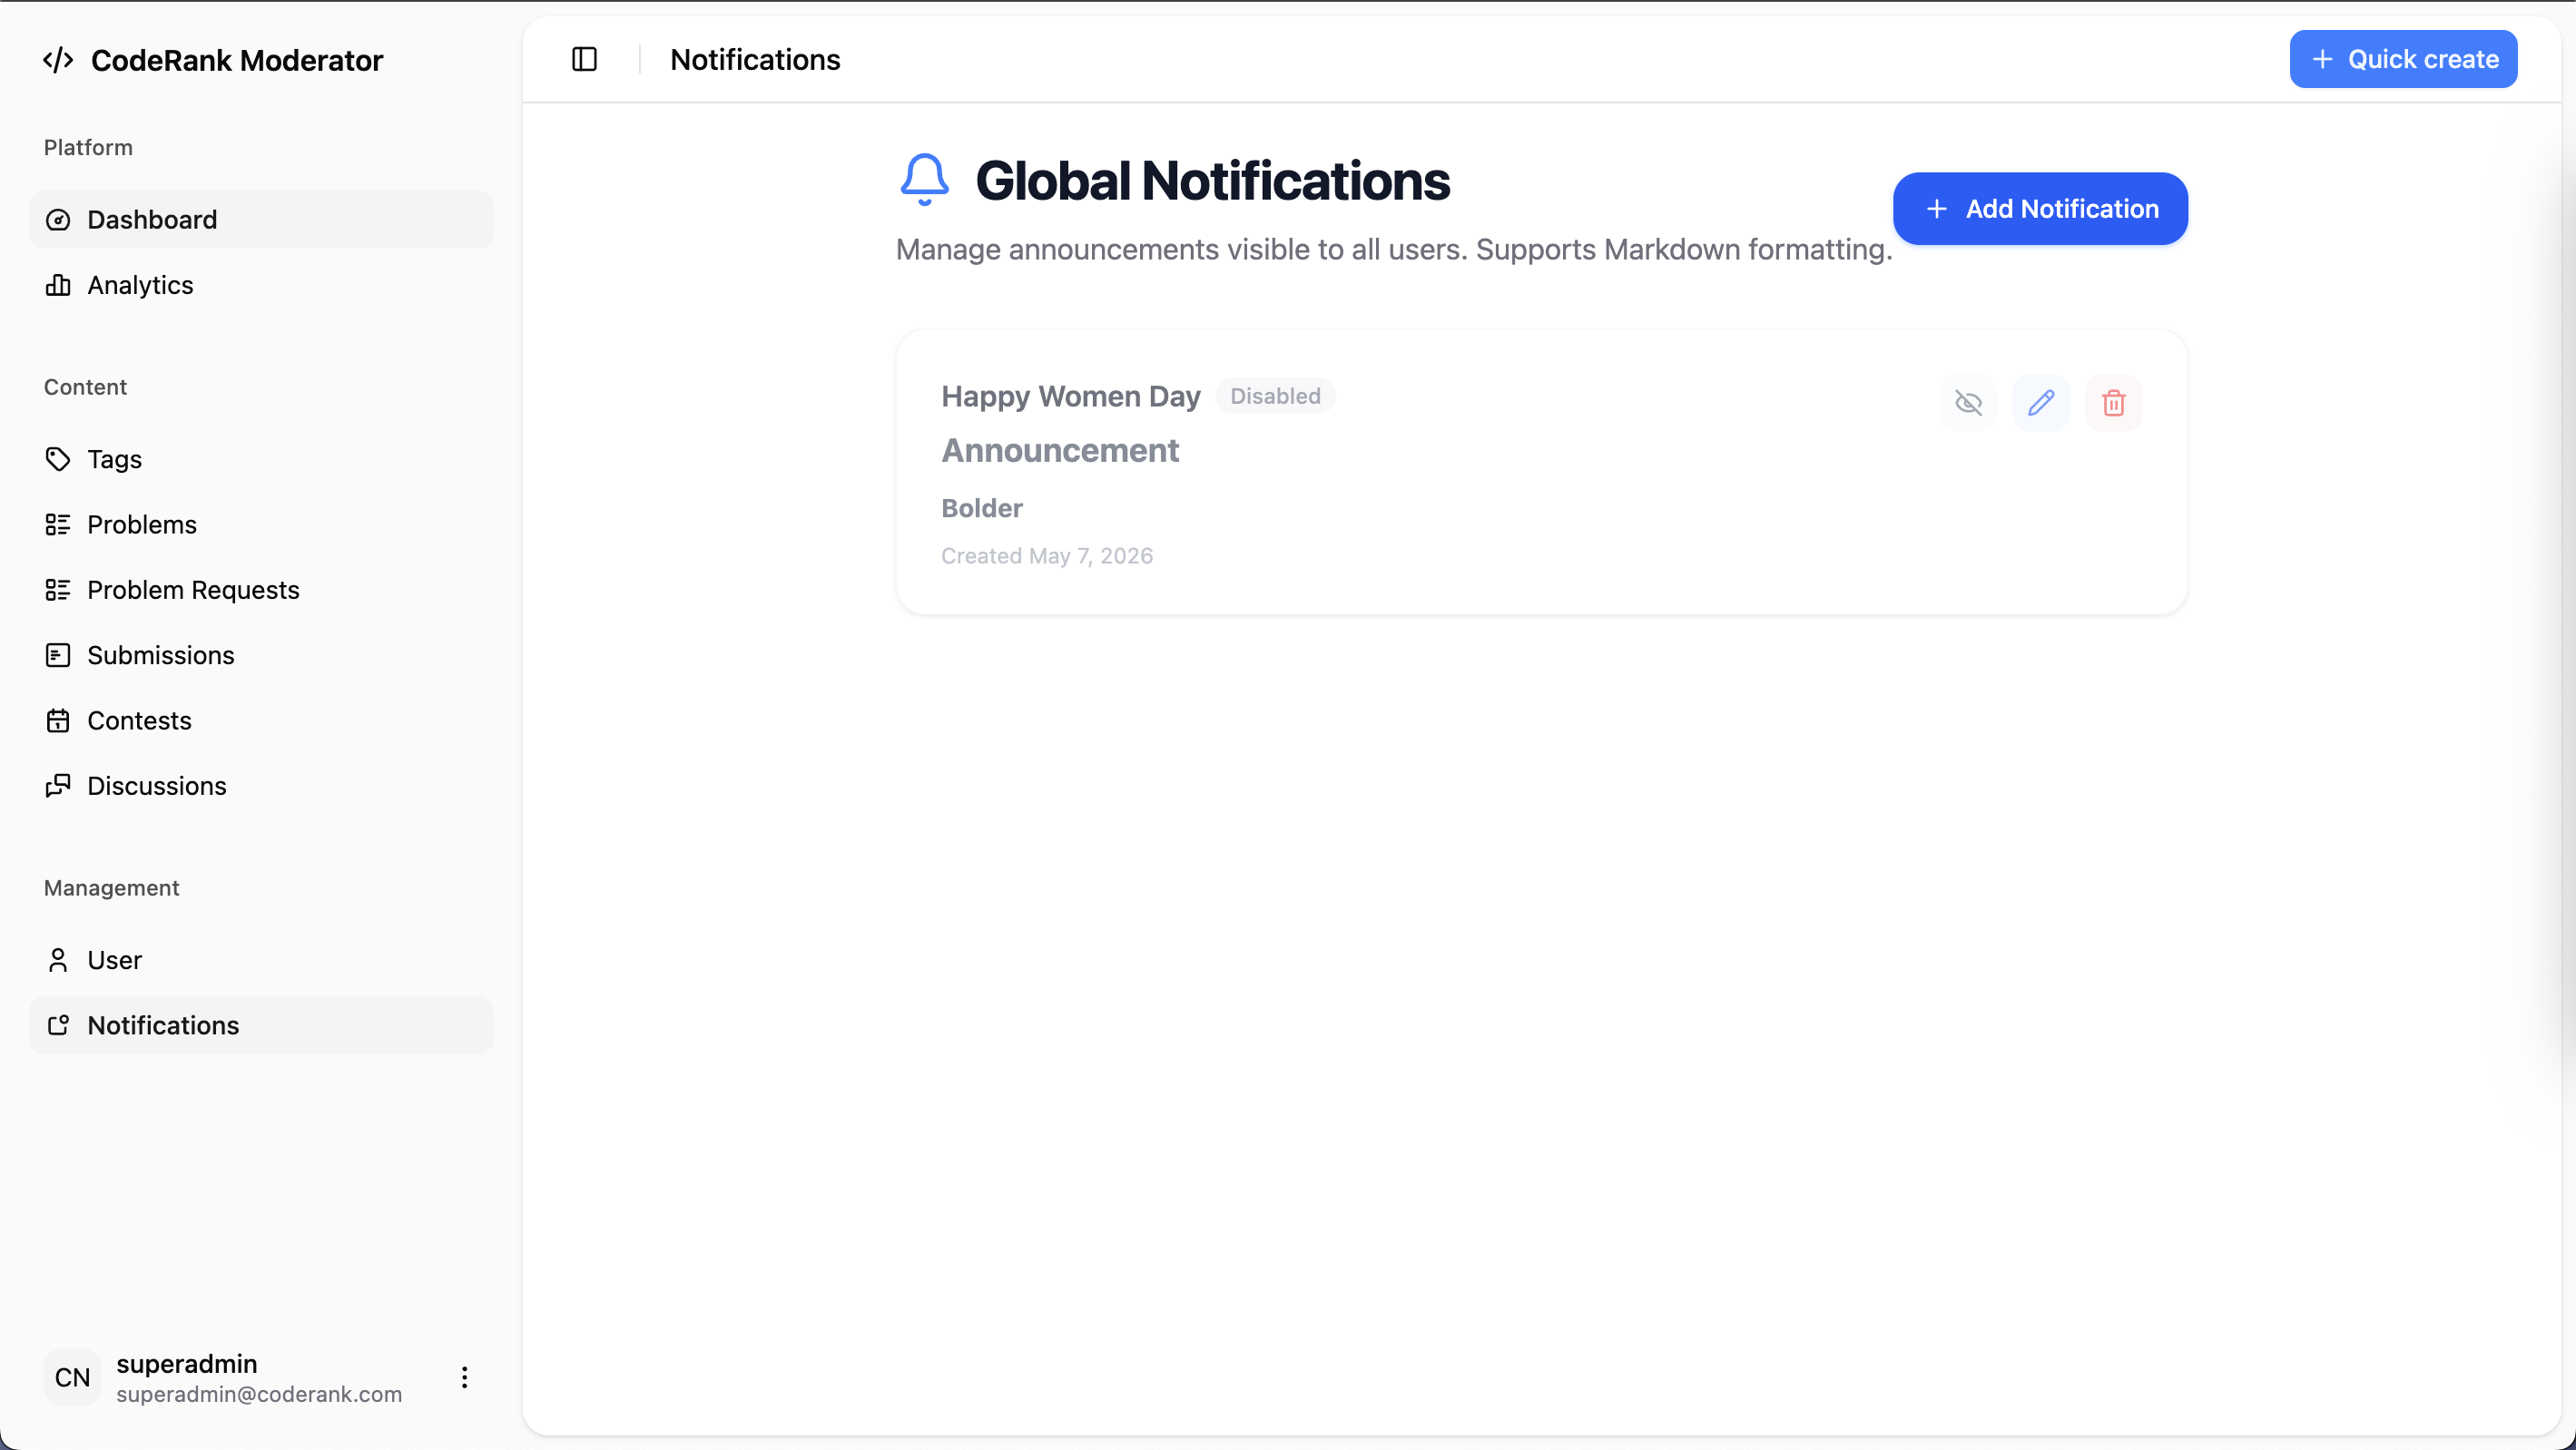
\includegraphics[width=1\textwidth]{Contents/Chapter 4/Mockup Design/Admin/app_notification.png}
    \vspace{0.6cm}
    \caption{Notification Setting}
\end{figure}

% \section{Chatbot Implementation}

This section describes the detailed implementation of the chatbot subsystem in the CodeRank system. The implementation focuses on enabling real-time, streaming-based conversational interaction between the user and the AI assistant.

The chatbot is implemented using a multi-layer architecture consisting of the frontend client, backend API server, n8n workflow engine, and Gemini large language model. A key feature of the system is the use of Server-Sent Events (SSE) to support streaming responses, providing a real-time chat experience similar to modern AI assistants.

\subsection{End-to-End Chatbot Request Flow}

When a user interacts with the chatbot, the system processes the request through the following sequence:

\begin{enumerate}
    \item The user submits a message from the frontend chatbot interface.
    
    \item The frontend immediately sends the message to the backend API server using an HTTP request.
    
    \item The backend receives the request and initiates a processing pipeline by calling an internal chatbot service.
    
    \item The backend triggers an n8n workflow via a webhook, passing the user input and conversation metadata.
    
    \item n8n processes the request and communicates with the Gemini model to generate a response.
    
    \item The response is streamed back from n8n to the backend.
    
    \item The backend forwards the streamed response to the frontend using Server-Sent Events (SSE).
    
    \item The frontend renders the response incrementally in real time as tokens are received.
\end{enumerate}

This architecture ensures low-latency interaction and improves user experience by allowing the response to appear progressively instead of waiting for the full output.

\subsection{Backend Processing and Streaming Architecture}

The backend plays a critical role in managing request orchestration and enabling real-time response streaming.

After receiving the request from the frontend, the backend does not wait for the full response from the AI pipeline. Instead, it establishes a Server-Sent Events (SSE) connection with the client and acts as a streaming proxy between n8n and the frontend.

The backend performs the following tasks:

\begin{itemize}
    \item Validates incoming chatbot requests
    \item Forwards the request to the n8n webhook endpoint
    \item Receives streamed response chunks from n8n
    \item Forwards each chunk to the frontend via SSE channel
\end{itemize}

This streaming mechanism allows the system to handle long AI-generated responses efficiently while maintaining responsiveness.

\subsection{n8n Workflow Execution and Streaming Response}

Within the n8n workflow, the chatbot request is processed through multiple stages including context retrieval, prompt construction, and LLM inference.

Unlike traditional synchronous APIs, the integration is designed to support incremental response generation. As the Gemini model produces output, n8n streams partial results back to the backend instead of waiting for the full completion.

This streaming behavior is essential for enabling real-time chat experiences and reducing perceived latency.

The workflow acts as an intermediate layer that:
\begin{itemize}
    \item Receives user input from the backend via webhook
    \item Processes conversational context and memory
    \item Sends structured prompts to the Gemini model
    \item Streams generated tokens or response chunks back to the backend
\end{itemize}

\subsection{Frontend Streaming with Server-Sent Events (SSE)}

On the frontend side, the chatbot interface establishes a persistent SSE connection with the backend.

When a user sends a message, the frontend immediately displays a loading state and begins listening for streamed response events.

As the backend receives chunks of data from n8n, it forwards them to the frontend incrementally. The frontend then appends each received chunk to the chat interface in real time.

This results in a typewriter-like effect where the response appears progressively, significantly improving user experience compared to traditional request-response models.

The SSE-based approach provides the following benefits:
\begin{itemize}
    \item Low latency response rendering
    \item Improved perceived system performance
    \item Smooth real-time interaction experience
    \item Reduced waiting time for long AI outputs
\end{itemize}
